\documentclass[12pt,a4paper]{article}

%\usepackage[colorlinks=true, linkcolor=black!50!blue, urlcolor=blue, citecolor=blue, anchorcolor=blue]{hyperref}
\usepackage[font=small,labelfont=bf,margin=0mm,labelsep=period,tableposition=top]{caption}
\usepackage[a4paper,top=3cm,bottom=3cm,left=2.5cm,right=2.5cm,bindingoffset=0mm]{geometry}

\usepackage{graphicx,ragged2e}
\usepackage{float}
\usepackage{afterpage}
\usepackage{epsfig,cite}
\usepackage{amssymb}
\usepackage{amsmath}
\usepackage{bm}
\usepackage{dsfont}
\usepackage{multirow}
\usepackage{url}
\usepackage{xcolor}
\usepackage{float}
\usepackage{afterpage}
\usepackage{ulem}
\usepackage{url}
\usepackage{multirow,booktabs,multirow}
\bibliographystyle{JHEP}

%%%%%%%%%%%%%%%%%%%%%%%%%%%%%%%%%%%%%%%%%%%%%%%%%%%%%%%%%%%%%

\def\smallfrac#1#2{\hbox{$\frac{#1}{#2}$}}
\newcommand{\be}{\begin{equation}}
\newcommand{\ee}{\end{equation}}
\newcommand{\bea}{\begin{eqnarray}}
\newcommand{\eea}{\end{eqnarray}}
\newcommand{\ei}{\end{itemize}}
\newcommand{\ben}{\begin{enumerate}}
\newcommand{\een}{\end{enumerate}}
\newcommand{\la}{\left\langle}
\newcommand{\ra}{\right\rangle}
\newcommand{\lc}{\left[}
  \newcommand{\tr}{\toprule}
  \newcommand{\mr}{\midrule}
  \newcommand{\br}{\bottomrule}
\newcommand{\rc}{\right]}
\newcommand{\lp}{\left(}
\newcommand{\rp}{\right)}
\newcommand{\as}{\alpha_s}
\newcommand{\aq}{\alpha_s\left( Q^2 \right)}
\newcommand{\amz}{\alpha_s\left( M_Z^2 \right)}
\newcommand{\aqq}{\alpha_s \left( Q^2_0 \right)}
\newcommand{\aqz}{\alpha_s \left( Q^2_0 \right)}
\def\toinf#1{\mathrel{\mathop{\sim}\limits_{\scriptscriptstyle
{#1\rightarrow\infty }}}}
\def\tozero#1{\mathrel{\mathop{\sim}\limits_{\scriptscriptstyle
{#1\rightarrow0 }}}}
\def\toone#1{\mathrel{\mathop{\sim}\limits_{\scriptscriptstyle
{#1\rightarrow1 }}}}
\def\frac#1#2{{{#1}\over {#2}}}
\def\gsim{\mathrel{\rlap{\lower4pt\hbox{\hskip1pt$\sim$}}
    \raise1pt\hbox{$>$}}}       
\def\lsim{\mathrel{\rlap{\lower4pt\hbox{\hskip1pt$\sim$}}
    \raise1pt\hbox{$<$}}}       
\newcommand{\mrexp}{\mathrm{exp}}
\newcommand{\dat}{\mathrm{dat}}
\newcommand{\one}{\mathrm{(1)}}
\newcommand{\two}{\mathrm{(2)}}
\newcommand{\art}{\mathrm{art}}
\newcommand{\rep}{\mathrm{rep}}
\newcommand{\net}{\mathrm{net}}
\newcommand{\stopp}{\mathrm{stop}}
\newcommand{\sys}{\mathrm{sys}}
\newcommand{\stat}{\mathrm{stat}}
\newcommand{\diag}{\mathrm{diag}}
\newcommand{\pdf}{\mathrm{pdf}}
\newcommand{\tot}{\mathrm{tot}}
\newcommand{\minn}{\mathrm{min}}
\newcommand{\mut}{\mathrm{mut}}
\newcommand{\partt}{\mathrm{part}}
\newcommand{\dof}{\mathrm{dof}}
\newcommand{\NS}{\mathrm{NS}}
\newcommand{\cov}{\mathrm{cov}}
\newcommand{\gen}{\mathrm{gen}}
\newcommand{\cut}{\mathrm{cut}}
\newcommand{\parr}{\mathrm{par}}
\newcommand{\val}{\mathrm{val}}
\newcommand{\reff}{\mathrm{ref}}
\newcommand{\Mll}{M_{ll}}
\newcommand{\extra}{\mathrm{extra}}
\newcommand{\draft}[1]{}
% Added by MU 
\def \a{\alpha}
\def \b{\beta}
\def \g{\gamma}
\def \z{\zeta}
\def \t{{\bf T}} % vector of theoretical predictions
\def \c{{\bf c}} % vector of coefficients of theoretical predictions
\def \y{{\bf y}} % vector of experimental data
\def \s{{\bf \sigma}} % experimental covariance matrix
% Added by JR
\def\lapprox{\lower .7ex\hbox{$\;\stackrel{\textstyle <}{\sim}\;$}}
\def\gapprox{\lower .7ex\hbox{$\;\stackrel{\textstyle >}{\sim}\;$}}
\def\half{\smallfrac{1}{2}}
\def\GeV{{\rm GeV}}
\def\TeV{{\rm TeV}}
\def\ap{{a'}}
\def\vp{{v'}}
\def\e{\epsilon}
\def\d{{\rm d}}
\def\calN{{\cal N}}
\def\shat{\hat{s}}
\def\barq{\bar{q}}
\def\qq{q \bar q}
\def\uu{u \bar u}
\def\dd{d \bar d}
\def\pp{p \bar p}
\def\xa{x_{1}}
\def\xb{x_{2}}
\def\xaa{x_{1}^{0}}
\def\xbb{x_{2}^{0}}
\def\smx{\stackrel{x\to 0}{\longrightarrow}}
\def\Li{{\rm Li}}
\numberwithin{equation}{section}
\numberwithin{figure}{section}
\numberwithin{table}{section}
\newcommand{\tmop}[1]{\ensuremath{\operatorname{#1}}}
\newcommand{\tmtextit}[1]{{\itshape{#1}}}
\newcommand{\tmtextrm}[1]{{\rmfamily{#1}}}
\newcommand{\tmtexttt}[1]{{\ttfamily{#1}}}
\usepackage{tabularx}
\newcolumntype{C}[1]{>{\centering\arraybackslash}p{#1}}
\begin{document}
\newgeometry{top=1.5cm,bottom=1.5cm,left=2.5cm,right=2.5cm,bindingoffset=0mm}

%\title[Charting Electron Energy Loss Spectroscopy with machine learning]{Charting the low-loss region in Electron Energy Loss Spectroscopy with machine learning}

%\author{}
%\address{}

%\ead{s.conesaboj@tudelft.nl}
%\vspace{10pt}
%\begin{indented}
%\item[]September 2020
%\end{indented}


\begin{flushright}
Nikhef/2020-022\\
\end{flushright}
\vspace{0.3cm}

\begin{center}
  {\Large \bf Automated data processing and feature identification\\[0.3cm] in
    EELS spectral images with machine learning}
\vspace{1.4cm}


author list

\vspace{1.0cm}
 
{\it \small

$^{1}$Kavli Institute of Nanoscience, Delft University of Technology, 2628CJ Delft, The
  Netherlands\\[0.1cm]
$^{2}$Nikhef Theory Group, Science Park 105, 1098 XG Amsterdam, The
  Netherlands \\[0.1cm]$^{3}$Department of Physics and Astronomy, VU,
    1081 HV Amsterdam, The Netherlands

}

\vspace{1.0cm}

{\bf \large Abstract}

\end{center}

Spectral images in Electron Energy Loss Spectroscopy (EELS) are two-dimensional
sets of spectra where each pixel corresponds a highly localised region of the analysed sample.
%
Here we present a novel approach to automated data processing and feature identification
in EELS spectral images based on machine learning.
%
The constituent spectra are clustered into groups of pixels associated
to sample regions with similar thickness using unsupervised learning,
and then the zero-loss peak (ZLP) is subtracted in a model-independent manner
by means of deep neural networks.
%
The resulting spectral images are  processed to determine 
local electronic properties such as
the band gap and the dielectric function across the sample,
which are then correlated  with the local thickness and other
relevant structural properties.
%
In addition to providing unique information on the direct correlation
between structural and electrical properties, our approach makes possible
the automated identification of interesting features
in the spectra (say a narrow peak)  then determine
how these features  (peak position and width) vary within different regions of the
sample.
%
This strategy, which can be straightforwardly extended
to higher-dimensional datasets,
is implemented into a new release of the open source
code {\tt EELSfitter}.


\vspace{0.4cm}
\noindent{\it Keywords:} {\small Transmission Electron Microscopy,
Electron Energy Loss Spectroscopy, Neural Networks, Machine Learning, Transition
Metal Dichalcogenides, Bandgap, Dielectric Function.}\\

\noindent
{\it $^{*}$corresponding author:} \url{s.conesaboj@tudelft.nl}

\clearpage
\tableofcontents


\section{Introduction}
\label{sec:introduction}

Electron energy-loss spectroscopy (EELS) within the transmission electron microscope (TEM) provides
a wide range of
valuable information on the structural, chemical, and electronic properties of nanoscale materials.
%
Thanks to recent instrumentation breakthroughs
such as electron monochromators~\cite{Terauchi:2005, Freitag:2005} and aberration correctors~\cite{Haider:1998},
modern EELS analyses can study these properties with highly competitive spatial and spectral resolution.
%
A particularly important region of EEL spectra is
the low-loss region, defined by electrons that have lost a few tens of eV,
$\Delta E\lsim 50$ eV,
following their inelastic interactions with the sample.
%
The analysis of this low-loss region makes possible charting the local
electronic properties of nanomaterials~\cite{Geiger:1967}, from the characterisation of
bulk and surface plasmons~\cite{Schaffer:2008}, excitons~\cite{Erni:2005}, 
inter- and intra-band transitions~\cite{Rafferty:1998},
and phonons to the determination of their bandgap and band structure~\cite{Stoger:2008}.

Provided the specimen is electron-transparent, as required for TEM inspection,
the bulk of the incident electron beam will traverse it
either without interacting or restricted to elastic scatterings with the atoms
of the sample's crystalline lattice.
%
In EEL spectra, these electrons are recorded as a narrow,
high intensity peak centered at energy losses
of $\Delta E\simeq 0$, known as the zero-loss peak (ZLP).
%
The energy resolution of EELS analyses is ultimately determined by
the electron beam size of the system, often expressed in terms
of the full width at half maximum (FWHM) of the
ZLP~\cite{Egerton:2009}.
%
In the low-loss region, the contribution from the ZLP
often overwhelms that from the inelastic scatterings arising from
the interactions of the beam electrons with the sample.
%
Therefore, relevant signals of low-loss phenomena such as excitons,
phonons, and intraband transitions risk becoming drowned
in the ZLP tail~\cite{Abajo:2010}.
%
An accurate removal of the ZLP
contribution is thus crucial in order to accurately chart and identify the features
of the low-loss region in EEL spectra.


In monochromated EELS, the properties of the ZLP depend on the electron energy dispersion,
the monochromator alignment, and the sample thickness~\cite{Park:2008, Stoger:2008}.
%
The first two factors arise already in the absence of a specimen (vacuum operation),
while the third is associated
to interactions with the sample such as atomic scatterings,
phonon excitation, and exciton losses.
%
This implies that EEL measurements in vacuum can be used for calibration purposes
but not to subtract the ZLP from spectra taken on specimens, since their shapes will
in general differ.




Several approaches to ZLP subtraction\cite{Rafferty:2000, Stoger:2008, Egerton:1996} 
have been put forward in the literature.
%
These are often based on specific model assumptions about the ZLP properties, in particular
concerning its parametric functional dependence on the electron energy loss $\Delta E$,
from Lorentzian~\cite{Dorneich:1998}
and power laws~\cite{Erni:2005} to more general multiple-parameter functions~\cite{Benthem:2001}.
%
Another approach is based on mirroring the $\Delta E <0$ region of the spectra, assuming
that the $\Delta E>0$ region is fully symmetric~\cite{Lazar:2003}.
%
More recent studies use integrated software applications for background
subtraction~\cite{Egerton:10.1016/S0304-3991(01)00155-3, Held:2020, Granerod:2018, Fung:2020}.
%
These various methods are however affected by three main limitations.
%
Firstly, their reliance on model assumptions such as
the choice of fit function introduces a methodological
bias whose size is difficult to quantify.
%
Secondly, they lack an estimate of the associated uncertainties, which in turn affects
the reliability of any physical interpretations of the low loss region.
%
Thirdly, {\it ad hoc} choices such as those of the fitting ranges introduce a significant degree of
arbitrariness in the procedure.



In this study we bypass these limitations by developing a model-independent strategy
to realise a multidimensional determination of the ZLP
with a faithful uncertainty estimate.
%
Our approach is based on machine learning (ML) techniques
originally developed in high-energy physics to study the
quark and gluon substructure of protons in particle collisions~\cite{Ball:2008by,Ball:2012cx,Ball:2014uwa,Ball:2017nwa}.
%
It is based on the Monte Carlo replica method to construct a probability
distribution in the space of experimental data and artificial
neural networks as unbiased interpolators to parametrise the ZLP.
%
The end result is
a faithful sampling of the probability distribution in the ZLP space 
which can be used to subtract its contribution to EEL spectra while
propagating the associated uncertainties.
%
One can also extrapolate the predictions from this ZLP parametrisation to other TEM
operating conditions beyond those included in the training dataset.



This work is divided into two main parts.
%
In the first one, we construct a ML model of ZLP spectra acquired
in vacuum, which is able to accommodate an arbitrary number of input
variables corresponding to different operation settings of the TEM.
%
We demonstrate how this model successfully describes the
input spectra and we assess its extrapolation capabilities for other operation
conditions.
%
In the second part, we construct a one-dimensional model
of the ZLP as a function of $\Delta E$ from spectra acquired on two different specimens of
tungsten disulfide (WS$_2$) nanoflowers characterised by a 2H/3R mixed polytypism~\cite{SabryaWS2}.
%
The resulting subtracted spectra are used to determine
the value and nature of the WS$_2$ bandgap in these nanostructures
as well as to map the properties of the associated exciton peaks appearing in the ultra-low
loss region.



This paper is organized as follows.
%
First of all, in Sect.~\ref{sec:tmdeels}
we review the main features of EELS and present
the WS$_2$ nanostructures that will be used as proof of concept of our approach.
%
In Sect.~\ref{sec:methodology} we describe the machine learning methodology
adopted to model the ZLP features.
%
Sects.~\ref{sec:results_vacuum} and~\ref{sec:results_sample} contain
the results of the ZLP parametrisation of spectra acquired
in vacuum and in specimens respectively, which in the latter
case allows us to probe the local electronic properties properties
of the WS$_2$ nanoflowers.
%
Finally in Sect.~\ref{sec:summary} we summarise
and outline possible future developments.
%
Our results have been obtained with an open-source {\sc Python} code,
dubbed {\tt EELSfitter}, whose installation and usage instructions
are described in Appendix~\ref{sec:installation}.

%%%%%%%%%%%%%%%%%%%%%%%%%%%%%%%%%%%%%%%%%%%%%%%%%%%%%%
\section{Neural network determination of the ZLP}
%%%%%%%%%%%%%%%%%%%%%%%%%%%%%%%%%%%%%%%%%%%%%%%%%%%%%
\label{sec:methodology}

In this section we present our strategy to parametrise and subtract in a model-independent manner
the zero-loss peak that arises in the low-loss region of EEL spectra by means
of machine learning.
%
As mentioned in the introduction, our strategy will be inspired by the 
NNPDF method~\cite{Rojo:2018qdd} originally developed in the context of high-energy physics
for studies of the quark and gluon substructure of the proton~\cite{Gao:2017yyd}.
%
The NNPDF approach has been successfully applied, among others, to
the determination of
unpolarised~\cite{DelDebbio:2007ee,Ball:2008by,Ball:2012cx,Ball:2014uwa,Ball:2017nwa}
and polarised parton distributions functions of protons,  nuclear
parton distributions~\cite{AbdulKhalek:2019mzd,AbdulKhalek:2020yuc}, and the
fragmentation functions of partons into neutral and charged
hadrons~\cite{Bertone:2017tyb,Bertone:2018ecm}.

We note that recently several applications of machine learning
to transmission electron microscopy analyses 
in the context of material science have been
presented, see {\it e.g.}~\cite{Gordon:2020, Zhang:2019, Jany:2017, Ziatdinov:2017,10.1145/2834892.2834896,doi:10.1021/acsnano.7b07504,cite-key}.
%
Representative examples
include the automated identification
of atomic-level structural information~\cite{10.1145/2834892.2834896},
the extraction of chemical information
and defect classification~\cite{doi:10.1021/acsnano.7b07504},
and spatial resolution enhancement
using  using a generative adversarial network~\cite{cite-key}.
%
To the best of our knowledge, this is
the first time that neural networks are used as 
 unbiased
 background-removal interpolators
 and combined with Monte Carlo sampling to construct a faithful estimate
of the model uncertainties.

In this section
first of all we discuss the parametrisation of the ZLP in terms of neural networks.
%
We then review the Monte Carlo replica method used to estimate and propagate the
uncertainties to the input data to the model predictions.
%
Subsequently, we present our training strategy both in case of vacuum and of sample spectra,
and discuss how one can select the hyper-parameters that appear in the model.

\subsection{ZLP parametrisation}
\label{sec:parametrisation}

To begin with we note that, without any loss of generality, the intensity profile
associated to an EEL spectrum may be decomposed as
\be
\label{eq:IeelTot}
I_{\rm EEL}(\Delta E) =I_{\rm ZLP}(\Delta E) + I_{\rm inel}(\Delta E) \, ,
\ee
where $\Delta E$ is the measured electron energy loss; $I_{\rm ZLP}$ is the zero-loss peak
distribution arising both from instrumental origin  and from elastic scatterings; and
$I_{\rm inel}(\Delta E)$ contains the contributions from the
inelastic scatterings off the electrons and atoms in the specimen.
%
As shown by the representative example of Fig.~\ref{fig:EELS}, there are two limits
for which one can cleanly disentangle the two contributions.
%
First of all, for large enough values of
$\Delta E$ then
$I_{\rm ZLP}$ vanishes and thus $I_{\rm EEL} \to I_{\rm inel}$.
%
Secondly, in the $\Delta E\simeq 0$ limit all emission can be associated to
 the ZLP such that $I_{\rm EEL}\to  I_{\rm ZLP}$.
%
In this work we are interested in the ultra-low-loss region, where $I_{\rm ZLP}$ and $I_{\rm inel}$
become of the comparable magnitude.

Our goal is to construct a parametrisation of $I_{\rm ZLP}$ based on artificial
neural networks, which we denote by $I_{\rm ZLP}^{\rm (mod)}$, whereby we
can extract the relevant inelastic contribution by subtracting the
ZLP background to the measured intensity spectra,
\be
\label{eq:ZLPseparation}
I_{\rm inel}(\Delta E) \simeq I_{\rm EEL}(\Delta E) - I_{\rm ZLP}^{\rm (mod)}(\Delta E) \, ,
\ee
and thus be able to exploit the physical information contained in $I_{\rm inel}$ in
the low-loss region.
%
Crucially, we aim to faithfully estimate and propagate all the relevant sources of uncertainty associated
both to the input data and to methodological choices.

As discussed in Sect.~\ref{sec:eels}, the ZLP depends both
on the value of the electron energy loss $\Delta E$ as well as on the operation
parameters of the microscope, such as the electron beam energy $E_b$ and the exposure time
$t_{\rm exp}$.
%
Therefore we want to construct a multidimensional model which takes all relevant
variables as input.
%
This means that in general Eq.~(\ref{eq:ZLPseparation}) must be written as
\be
I_{\rm inel}(\Delta E) = I_{\rm EEL}(\Delta E, E_{b},t_{\rm exp}, \ldots) - I_{\rm ZLP}^{\rm (mod)}(\Delta E, E_{b},t_{\rm exp}, \ldots) \, ,
\ee
where we note that the subtracted spectra should depend only on $\Delta E$ but not on the microscope
operation parameters.
%
Ideally, the ZLP model should be able to accomodate as many input variables as possible.
%
Here we parametrise $I_{\rm ZLP}^{\rm (mod)}$ by means of
multi-layer feed-forward artificial neural networks, that is, we express our ZLP model as
\be
\label{eq:ZLPmodelNN}
I_{\rm ZLP}^{\rm (mod)}(\Delta E, E_{b},t_{\rm exp}, \ldots)  = \xi^{(n_l)}_1(\Delta E, E_{b},t_{\rm exp}, \ldots) \, ,
\ee
where $\xi^{(n_l)}_1$ denotes the activation state of the single neuron in the last
of the $n_l$ layers of the network when the $n_I$ inputs $\{ \Delta E, E_{b},t_{\rm exp}, \ldots \}$
are used.
%
The weights and thresholds of this neural network model are then determined
from the maximization of the model likelihood by means
of supervised learning and non-linear regression from a suitable training dataset.
%
This type of neural networks benefit from the ability
to parametrise multidimensional input data with arbitrarily
non-linear dependencies: even with a single hidden layer, a neural network
can reproduce arbitrary functional dependencies provided it has a large enough
number of neurons.

A schematic representation of our model
is displayed in Fig.~\ref{fig:architecture}.
%
 The input is an $n_I$ array containing $\Delta E$ and the rest of
 operation variables of the microscope, and
 the output is the value of the intensity of the ZLP distribution
 associated to those input variables.
 %
 We adopt an $n_I$-10-15-5-1 architecture with three hidden layers, for a total
 number of 289~(271) free parameters for $n_I=3$~($n_I=1$) to be adjusted by the optimization procedure.
 %
 We use a sigmoid activation function for the three hidden layers and a ReLU
 for the final one.
 %
 The choice of ReLU for the final layer guarantees that our model for the ZLP
 is positive-definite, as required by general physical considerations.
 %
 We have adopted a redundant architecture  to ensure that the ZLP parametrisation
 is sufficiently flexible, and we avoid over-fitting by means of
 a suitable regularisation strategy, see Sect.~\ref{sec:training}.
  
%%%%%%%%%%%%%%%%%%%%%%%%%%%%%%%%%%%%%%%%%%%%%
\begin{figure}[t]
    \centering
    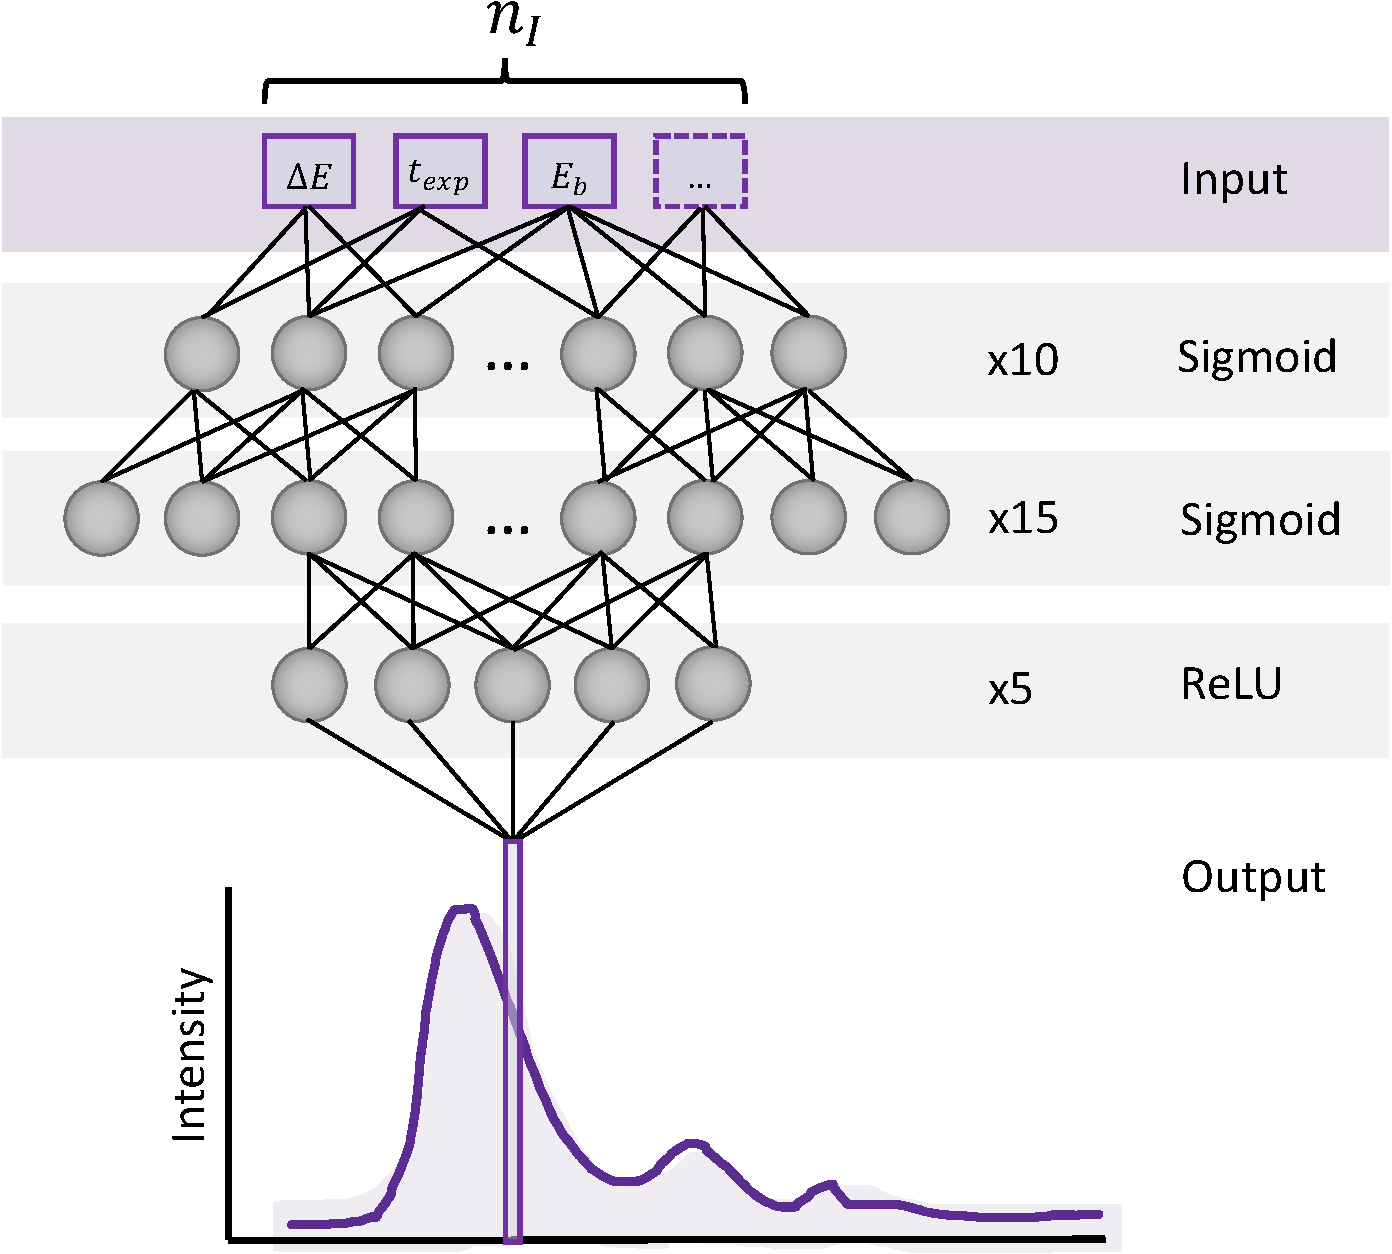
\includegraphics[width=99mm]{plots/architecture.pdf}
    \caption{Schematic representation of our ML model for the ZLP, Eq.~(\ref{eq:ZLPmodelNN}).
      %
      The input is an $n_I$-dimensional array containing $\Delta E$ and other
      operation variables of the microscope such as $E_b$ and $t_{\rm exp}$.
      %
      The output is the predicted value of the intensity of the zero-loss peak
      distribution associated to those specific input variables.
      %
      The architecture is chosen to be $n_I$-10-15-5-1, with sigmoid activation functions
      in all layers except for a ReLU in the output neuron.
    }
    \label{fig:architecture}
\end{figure}
%%%%%%%%%%%%%%%%%%%%%%%%%%%%%%%%%%%%%%%%%%%%%%%%%

\subsection{Uncertainty propagation}

We discussed in Sect.~\ref{sec:eels} how
even for EEL spectra taken at identical operation conditions of the microscope,
in general the resulting ZLP intensities will differ.
%
Further, there exist a large number of different NN configurations, each
representing a different functional form for $I_{\rm ZLP}^{(\rm mod)}$ which provide
an equally valid description of the input data.
%
To  estimate these uncertainties and propagate them to physical predictions,
we use here the Monte Carlo replica method.
%
The basic idea  is to exploit the available information
on experimental measurements (central values, uncertainties, and correlations)
to construct a sampling of the probability density in the space of 
the data, which by means of the NN training is then propagated
to a probability density in the space of $I_{\rm ZLP}$ models.

Let us assume that we have $n_{\rm dat}$ independent measurements of the ZLP intensity, for
different or the same values of the input parameters collectively denoted as $\{z_i\}$:
\be
I^{\rm (exp)}_{{\rm ZLP},i}\lp \{ z_i  \}\rp = I^{\rm (exp)}_{{\rm ZLP},i}\lp  \Delta E_i, E_{b,i}, t_{\rm exp,i},\ldots \rp
\,, \quad i=1,\ldots,n_{\rm dat} \, .
\ee
The Monte Carlo method is based on the generation
of a large number $N_{\rm rep}$ of Monte Carlo replicas of these original data points
by means of a multi-Gaussian distribution, with the central values and covariance matrices
from the input measurements,
\be
\label{eq:MCreplicaGen}
  I_{{\rm ZLP},i}^{{\rm (art)}(k)}  =  I^{\rm (exp)}_{{\rm ZLP},i} + r_i^{({\rm stat},k)}\sigma_i^{\rm (stat)}
  + \sum_{j=1}^{n_{\rm sys}} r_{i,j}^{({\rm sys},k)} \sigma_{i,j}^{\rm (\rm sys)} \,, \quad \forall i
  \,, \quad k=1,\ldots,N_{\rm rep} \,.\,\, \,
  \ee
  where $\sigma_i^{\rm (stat)}$ and $\sigma_{i,j}^{\rm (\rm sys)}$ represent the statistical
  and systematic uncertainties (the latter divided into  $n_{\rm sys}$ fully point-to-point correlated
  sources) and $\{r_i^{(k)}\}$ are Gaussianly distributed random numbers.
  %
  The values of $\{r_i^{(k)}\}$ are
  generated with a suitable correlation pattern to ensure
  that averages over the set of Monte Carlo
  replicas reproduce the original experimental covariance matrix, namely
  \be
  \la  \lp I_{{\rm ZLP},i}^{{\rm (art)}(k)} - \la I_{{\rm ZLP},i}^{{\rm (art)}}\ra_{\rm rep}\rp
  \lp I_{{\rm ZLP},j}^{{\rm (art)}(k)} - \la I_{{\rm ZLP},j}^{{\rm (art)}}\ra_{\rm rep}\rp\ra_{\rm rep}
  \label{eq:expcovariance} = {\rm cov}^{(\rm exp)}\lp I_{{\rm ZLP},i},I_{{\rm ZLP},j}\rp  \, ,
  \ee
  where averages are evaluated over the $N_{\rm rep}$ replicas that compose the sample.
  %
We thus note that each $k$-th replica contains 
as many data points as the original set.

In our case the information on experimental correlations is not accessible and
thus we assume that there is a single source of point-by-point uncorrelated systematic
uncertainty, denoted as $\sigma_i^{\rm (exp)}$, which is estimated as follows.
%
The input measurements will be composed in general on subsets of EEL
spectra taken with identical operation conditions.
%
Assume that for a specific set of operation conditions we have $N_{\rm sp}$ of such spectra.
%
Since the values of $\Delta E$ will be different in each case, first of all
we uniformise a common binning in $\Delta E$ with $n_{\rm dat}$ entries.
%
Then we evaluate the total experimental uncertainty in one of these bins as
\be
\label{eq:sigmaiexp}
\sigma_i^{\rm (exp)} = \lp \frac{1}{N_{\rm sp}-1} \sum_{l=1}^{N_{\rm sp}}
\lp I_{{\rm ZLP},i}^{ ({\rm exp}),l}  - \la I_{{\rm ZLP},i}^{ ({\rm exp})}\ra_{N_{\rm sp}} \rp \rp^{1/2} \, ,\,
i=1,\ldots, n_{\rm dat} \, ,
\ee
that is, as the standard deviation over the $N_{\rm sp}$ spectra.
%
This uncertainty is separately evaluated for each set of microscope operation conditions
for which data available.
%
In the absence of correlations Eqns.~(\ref{eq:MCreplicaGen}) and~(\ref{eq:expcovariance}) thus
simplify to
\be
 I_{{\rm ZLP},i}^{{\rm (art)}(k)}  =  I^{\rm (exp)}_{{\rm ZLP},i} + r_i^{({\rm tot},k)}\sigma_i^{\rm (exp)}
 \,, \quad \forall i
  \,, \quad k=1,\ldots,N_{\rm rep} \,.\,\, \,
\ee
and
  \bea
  \la  \lp I_{{\rm ZLP},i}^{{\rm (art)}(k)} - \la I_{{\rm ZLP},i}^{{\rm (art)}}\ra_{\rm rep}\rp
  \lp I_{{\rm ZLP},j}^{{\rm (art)}(k)} - \la I_{{\rm ZLP},j}^{{\rm (art)}}\ra_{\rep}\rp\ra_{\rm rep} =
  \sigma_i^{\rm (exp)}\sigma_j^{\rm (exp)}\delta_{ij} \, ,
  \eea
  given that the experimental covariance matrix is diagonal.
  %
  Should in the future correlations became available, it would be straightforward to extend
  our model to that case.

The value of the number of generated MC replicas, $N_{\rm rep}$, should be chosen such that the set of replicas 
models accurately the probability distribution of original training data.
%
To verify that this is the case,
Fig.~\ref{fig:MC} displays a comparison between the original experimental central values
$I_{{\rm ZLP},i}^{\rm (exp)}$ (left) and the corresponding 
total uncertainties $\sigma_i^{(\rm exp)}$ (right panel) with the results of averaging over
a sample of $N_{\rm rep}$ Monte Carlo replicas generated by means of
Eq.~(\ref{eq:MCreplicaGen}) for different number of replicas.
%
We find that $N_{\rm rep}=500$ is a value that ensures that both
the central values and uncertainties are reasonably well reproduced,
and we adopt it in what follows.

%%%%%%%%%%%%%%%%%%%%%%%%%%%%%%%%%%%%%%%%%%%%%%%
\begin{figure}[t]
    \centering
    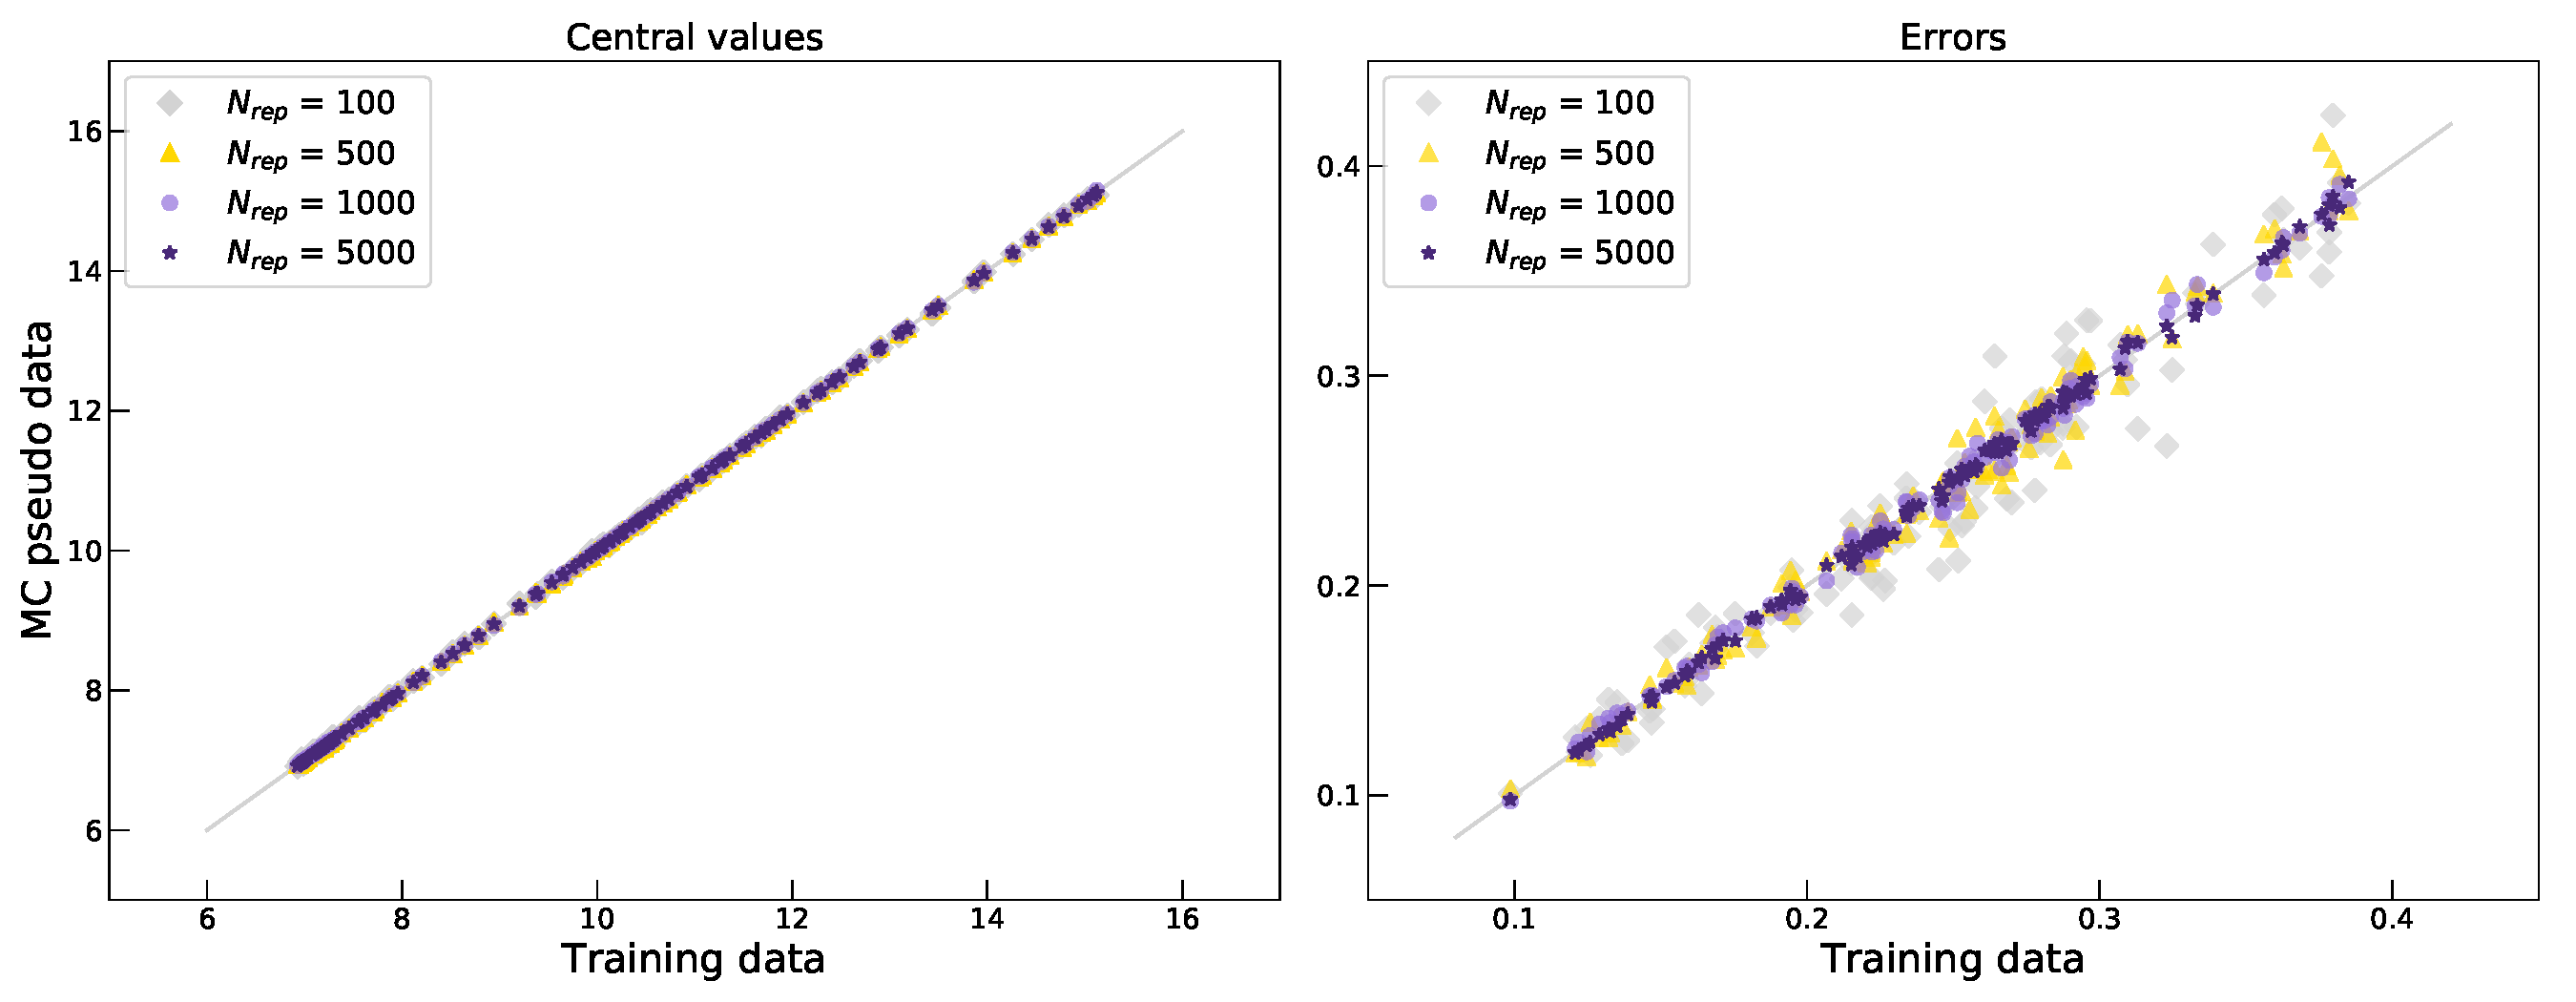
\includegraphics[width=0.99\textwidth]{plots/MC.pdf}
    \caption{Comparison between the original experimental central values
      $I_{\rm ZLP,i}^{\rm exp}$ (left panel) and the corresponding statistical
      uncertainties $\sigma_i^{(\rm stat)}$ with the results of averaging over
      a sample of $N_{\rm rep}$ Monte Carlo replicas generated by means of
      Eq.~(\ref{eq:MCreplicaGen}), for different values of
      $N_{\rm rep}$.
      }
    \label{fig:MC}
\end{figure}
%%%%%%%%%%%%%%%%%%%%%%%%%%%%%%%%%%%%%%%%%%%%%%%%5

\subsection{Training strategy}
\label{sec:training}

The training of the neural-network model for the ZLP peak differs between
the cases of EEL spectra taken on vacuum, where by construction $I_{\rm EEL}(\Delta E) =I_{\rm ZLP}^{\rm (mod)}(\Delta E)$,
and for spectra taken on sample.\footnote{Actually EEL spectra taken in the vacuum but close
  to the sample might still receive inelastic contributions due to processes such as .... Here
  when we use vacuum spectra we consider exclusively those taken reasonably far from the surface
of the analysed nanostructures.}
%
In the latter case, as indicated by Eq.~(\ref{eq:ZLPseparation}), in order to avoid
biasing the results it is
important to ensure that the model is trained only on the region of the spectra
where the ZLP dominates over the inelastic scatterings.
%
We now describe the training strategy that is adopted in both cases.

\paragraph{Training of vacuum spectra.}
%
For each of the $N_{\rm rep}$ generated Monte Carlo replicas, we train an independent
neural network as described in Sect.~\ref{sec:parametrisation}.
%
The parameters of the neural network are determined from the minimisation of a figure of merit
defined as
\begin{equation}
  \label{eq:chi2}
\begin{centering}
  E^{(k)}\lp \{\theta^{(k)}\}\rp = \frac{1}{n_{\rm dat}}\sum_{i=1}^{n_{dat}}\left(\frac{ I_{{\rm ZLP},i}^{{\rm (art)}(k)} -
  I_{{\rm ZLP},i}^{{\rm (mod)}}\lp \{\theta^{(k)}\}\rp }{\sigma_i^{(\rm exp)}}\right)^2, 
\end{centering}
\end{equation}
which is the $\chi^2$ per data point comparing the $k$-th replica for the ZLP
intensity with the corresponding model prediction for the values
$\{\theta^{(k)}\}$ of its weights and thresholds.
%
In order to speed up the neural network training process, prior to the optimisation
all inputs and outputs are scaled to lie between $[0.1, 0.9]$ before
being feed to the network.
%
This preprocessing facilitates that
 the neuron activation states will typically
lie close to the linear region of the sigmoid activation function.

The contribution to the figure of merit from the input experimental data, Eq.~(\ref{eq:chi2}),
needs in general to be complemented with that of theoretical constraints on the model.
%
For instance, when determining nuclear parton distributions~\cite{AbdulKhalek:2020yuc}, one needs to
extend Eq.~(\ref{eq:chi2}) with Lagrange multipliers to ensure that both the $A=1$ proton boundary
condition and the cross-section positivity are satisfied.
%
In the case at hand, our model for the ZLP should implement the property that $I_{\rm ZLP}(\Delta E)\to 0$
when $|\Delta E| \to \infty$, since far from $\Delta E\simeq 0$ the contribution from elastic scatterings
and instrumental broadening is completely negligible.
%
In order to implement this constraint, we add $n_{pd}$ pseudo-data points to the training dataset and modify
the figure of merit Eq.~(\ref{eq:chi2}) as follows
\be
\label{eq:chi2modified}
E^{(k)}\lp \{\theta^{(k)}\}\rp \to E^{(k)}\lp \{\theta^{(k)}\}\rp +
\lambda \sum_{i'=1}^{n_{pd}}\left(
  I_{{\rm ZLP},i'}^{{\rm (mod)}}\lp \{\theta^{(k)}\}\rp \right)^2, 
  \ee
  where $\lambda$ is a Lagrange multiplier whose value is tuned to ensure that the $I_{\rm ZLP}(\Delta E)\to 0$
  condition
  is satisfied without affecting the description of the training dataset.
  %
  The pseudo-data points are chosen to lie in the region $\lc \Delta E_{\rm pd}^{\rm (min)},
  \Delta E_{\rm pd}^{\rm (max)}\rc$ (and symmetrically for negative energy losses),
  which is determined automatically via the ratio of the intensity to the uncertainty in each data point: 
  $I_{ZLP,i}^{(exp)} / \sigma_{i}^{(exp)}$. 
  %
  At a certain energy loss this ratio approaches 1, which indicates that we are practically fitting noise. 
  %
  In order to avoid this and only fit data that is different from zero within errors, we set the value
  of $\Delta E_{\rm pd}^{\rm (min)}$ for each set of training data equal to the point where the ratio
  $I_{ZLP,i}^{(exp)} / \sigma_{i}^{(exp)}$ drops below 1. 
  %
  We keep the training data in the region $\Delta E \le \Delta E_{\rm pd}^{\rm (min)}$ and the pseudo-data
  points are added for $\lc \Delta E_{\rm pd}^{\rm (min)}, \Delta E_{\rm pd}^{\rm (max)}\rc$. 
  %
  The value of $\Delta E_{\rm pd}^{\rm (max)}$ can be chosen arbitrarily and can be as large as necessary
  to ensure that $I_{\rm ZLP}(\Delta E)\to 0$ as $|\Delta E| \to \infty$.
  %u
We note that another important physical condition on the ZLP model, namely its positivity
(since in EEL spectra the intensity is just a measure of the number of counts in the
detector for a given value of the energy loss) is automatically satisfied since
we use a ReLU activation function for the last layer.

In this work we adopt the {\tt TensorFlow} neural-net libraries to assemble
the architecture illustrated in  Fig.~\ref{fig:architecture}.
%
Before training, all weights and biases are initialized in a non-deterministic order
by the built-in global variable initializer. 
%
The optimisation of the figure of merit Eq.~(\ref{eq:chi2modified}) is carried
out by means of stochastic gradient descent combined with backpropagation,
in particular by means of the Adam algorithm.
%
The hyper-parameters of the optimisation algorithm such as the learning rate
have been adjusted to ensure proper learning is reached in the shortest amount
of time possible.
%

Given that we have a extremely flexible parametrisation, one should be careful
to avoid overlearning the input data.
%
Here over-fitting is avoided by means of a cross-validation stopping criterion.
%
We separate the input data into training a validation subsets, with a 80\%/20\% splitting
which varies randomly for each Monte Carlo replica.
%
We then run the optimiser for a very large number of iterations and store both
the state of the network and the value
of the figure of merit Eq.~(\ref{eq:chi2}) restricted to the validation
dataset, $E^{(k)}_{\rm val}$ (which is not used for the training).
%
The optimal stopping point is then determined {\it a posteriori} for each replica
as the specific network configuration that leads to the deepest minimum of $E^{(k)}_{\rm val}$.
%
The number of epochs should be chosen high enough to reach the optimal stopping point for each replica.
For this work we need approximately 40,000 epochs to ensure overlearning.
%
This corresponds to a running time of 60 seconds per replica when training on a set of 500 datapoints.
%
Once the training of all the $N_{\rm rep}$ neural network models for the ZLP has been carried
out as specified above, we gauge the overal fit quality of the model by computing the
$\chi^2$ defined as
\begin{equation}
  \label{eq:chi2_final}
\begin{centering}
  \chi^2 = \frac{1}{n_{\rm dat}}\sum_{i=1}^{n_{dat}}\left(\frac{ I_{{\rm ZLP},i}^{{\rm (exp)}} -
 \la I_{{\rm ZLP},i}^{{\rm (mod)}}\ra_{\rm rep} }{\sigma_i^{(\rm exp)}}\right)^2, 
\end{centering}
\end{equation}
which is the analog of Eq.~(\ref{eq:chi2_final}) now comparing the average model prediction
to the original experimental data values.
%
A value $\chi^2 \simeq 1$ indicates that a satisfactory description of the experimental data,
within the corresponding uncertainties, has been achieved.
%
Note that in realistic scenarios $\chi^2$ can deviate from unity, for instance when
some source of correlation between the experimental uncertainties has been neglected.

\paragraph{Training of sample spectra.}

The training strategy in the case of EEL spectra taken on samples (rather than on vacuum) must be adjusted
to account for the fact that the input data set, Eq.~(\ref{eq:IeelTot}), receives contributions
both from the ZLP and from inelastic scatterings.
%
To avoid biasing the ZLP model, only the former contributions should be
included in the training dataset.

We can illustrate the situation here with the help of a toy model for the low-loss
region of EEL spectra, represented in
Fig.~\ref{fig:EELS_toy}.
%
Let us assume that the ZLP is described by a Gaussian distribution with a standard deviation of $\sigma_{\rm ZLP}=0.3$ eV,
and that the contribution from the
inelastic scatterings arising from the sample can be approximated in the low-loss
region by $I_{\rm inel}(\Delta E)\propto \lp \Delta E - E_{\rm bg}\rp^b$ with $E_{\rm bg}=1.5$
and $b=0.5$ -- the motivation for this
choice will be spelled out in Sect.~\ref{sec:results_sample}.
%
We display the separate contributions from $I_{\rm ZLP}$
and $I_{\rm inel}$, as well as their sum, 
with the inset showing the values of the corresponding derivatives, $dI/d\Delta E$.

%%%%%%%%%%%%%%%%%%%%%%%%%%%%%%%%%%%%%%%%%%%%%
\begin{figure}[t]
    \centering
    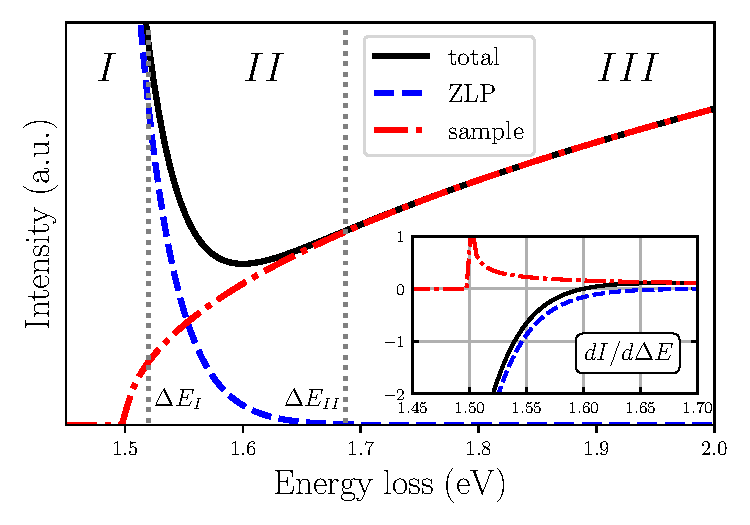
\includegraphics[width=0.89\textwidth]{plots/EELS_toy.pdf}
    \caption{A toy model for the EEL spectrum and its
      derivative (in the inset).
      %
      We display the separate contributions from $I_{\rm ZLP}$
      and $I_{\rm inel}$ as well as their sum.
      %
      We indicate the two regions used for the model training ($I$ and $III$),
      while as discussed in the text the trained model is then
      extrapolated to region $II$, defined for $\Delta E_I \le \Delta E \le \Delta E_{II}$.
    }
    \label{fig:EELS_toy}
\end{figure}
%%%%%%%%%%%%%%%%%%%%%%%%%%%%%%%%%%%%%%%%%%%%%%%%%

The toy model of Fig.~\ref{fig:EELS_toy} is general enough so that one can draw
a number of useful considerations concerning the relation between $I_{\rm ZLP}$ and $I_{\rm inel}$
in realistic spectra:

\begin{itemize}

\item The ZLP intensity, $I_{\rm ZLP}(\Delta E)$, is a monotonically decreasing function
  and thus its derivative is always negative.

\item  The first local minimum of the total spectrum, $dI_{\rm EELS}/d\Delta E|_{\Delta E_{\rm min}}=0$, corresponds
  to a value of $\Delta E$ for which the contribution from the inelastic emissions is already
  sizable.

\item The value of $\Delta E$ for which $I_{\rm inel}$ starts to contribute to the total spectrum
  corresponds to the position where the intensity derivatives in-sample and in-vacuum  start to differ.
  %
  We note that a direct comparison between the overal magnitude of the sample and vacuum ZLP
  spectra is in general not possible, as explained in Sect.~\ref{sec:eels}. 
\end{itemize}

These considerations suggest that when training the ML model on EEL spectra taken on samples,
the following categorisation should de adopted:

\begin{enumerate}

\item For energy losses such that $\Delta E \le \Delta E_I$ (region $I$),
  the model training  proceeds in the same way as for the vacuum case
  via the minimisation of Eq.~(\ref{eq:chi2})

\item  
  For $\Delta E \ge \Delta E_{II}$ (region $III$), we use instead Eq.~(\ref{eq:chi2modified})
  without the contribution from the input data, since for such values
  of $\Delta E$ one has that $I_{\rm inel}\gg I_{\rm ZLP}$.
  %
  In other words, the only information that the region $III$ provides
  on the model is the one arising from the implementation
  of the constraint that $I_{\rm ZLP}(\Delta E\to \infty)\to 0$.

\item The EELS data  in region $II$, defined by  $\Delta E_I \le \Delta E \le \Delta E_{II}$,
  is excluded from the training dataset, given that in this region the contribution to $I_{\rm EEL}$
  coming from $I_{\rm inel}$ is significant.
  %
  There the model predictions are obtained from an interpolation
  of the predictions obtained in regions $I$ and $III$.

\end{enumerate}

This classification introduces two new hyper-parameters of our model, $\Delta E_I$ and
$\Delta E_{II}$, that need to be specified before the training.
%
They should satisfy $\Delta E_I \le \Delta E_{\rm min}$ and $\Delta E_{II} \ge \Delta E_{\rm min}$,
with $\Delta E_{\rm min}$ being the position of the first local minimum of $I_{\rm EEL}$.
%
As indicated by the toy spectra of Fig.~\ref{fig:EELS_toy}, a suitable value for $\Delta E_{I}$
would be somewhat above the onset of the inelastic contributions, to maximise
the amount of training data while ensuring that $I_{\rm EEL}$ is dominated
by $I_{\rm ZLP}$.

We can use the derivatives of the spectra, $dI_{\rm EEL}/d\Delta E$, to select suitable minimum and
maximum values for $\Delta E_I$. In order to select the value for $\Delta E_{II}$, we use the intensity
profiles of the vacuum recorded spectra. 
%
Concerning $\Delta E_I $, its minimum possible value is selected as the value where the derivate taken on the sample
data start to different significantly as compared to those spectra taken on vacuum.
%
This value is obtained by looking at the ratio of the derivatives of the spectra compared to the vacuum derivatives,
$R_{dI/d \Delta E} =  \left( \frac{dI_{\rm ZLP}/d\Delta E}{dI_{\rm EEL}/d\Delta E}\right)$. 
%
For low energy losses this ratio equals 1, but at some energy loss $\Delta E_{I,min}$ the
sample stops monotonically decreasing and the ratio deviates from 1. 
%
We know that the hyper-parameter $\Delta E_I$ should satisfy $\Delta E_{I,min} \le \Delta E_I \le \Delta E_{\rm min}$,
which corresponds to the region where $R_{dI/d \Delta E} \ne  1$ and $R_{dI/d \Delta E} \ge 0$.
%
The neural network will be trained on an array of $\Delta E_I$ values within this interval and 
the optimal choice will be determined {\it a posteriori} from the results.
%
Another important difference as compared to the training of the vacuum spectra is that each of the sample
spectra will have different values of $\Delta E_{\rm min}$ and thus of $\Delta E_I$. 
%
For this reason we calculate $\Delta E_{\rm min}$  for each of the sample spectra and we use the highest of these
as the maximum value for the hyper-parameter $\Delta E_I$. 
%
As we determine the best choice of $\Delta E_I$ after training for each of the spectra separately, 
we are sure to capture all suitable results and select the best value for each individual spectrum. 
%
Concerning $\Delta E_{II}$, its minimum value should mark the region where $I_{\rm ZLP}(\Delta E\to \infty)\to 0$. 
%
In order to implement this constraint, similar to the previous section we look at the ratio 
$I_{ZLP,i}^{(exp)}/ \sigma_i^{(exp)}$ to determine the energy loss $\Delta E_{\rm pd}$ at 
which the contributions from the ZLP vanish. 
%
As a measure, we use the energy loss value where the ratio $I_{ZLP,io}^{(exp)}/\sigma_i^{(exp)}$ drops below 1. 
%
We set the value of $\Delta E_{II}$ equal to this energy loss and add pseudo-data points for $\Delta E \ge \Delta E_{II}$.
%
Note that in this region the intensity of the ZLP is several orders of magnitude smaller than the intensity 
of the elastic emissions and therefore the exact choice of $\Delta E_{II}$ does not listen too closely.

\section{Results}
\label{sec:results_vacuum}

We now move to discuss the application of the strategy presented in the previous
section to the parametrisation of ZLP spectra acquired in vacuum.

Some of the plots that we need for this section are

A bunch of fits (by "fit" I mean the full model say with 500 "replicas" at least) for different values of DeltaE_I

A heat map plot showing the calculation bandgap across the spectral image, using the approach in Laurien paper

A heat map plot for the thickness, now computed with the deconvoluted spectra just as with the sum of intensities, checking that the results of the two approaches are consistent

A plot of the dielectric function (with uncertainties) for different locations in the spectral image (representative).

A 2D plot demonstrating that the model interpolates in a sensible manner in the "intensity input"

A heat map with the crossing of the x axis for the real (or was it the imaginary) part of the dielectric function across the image

Some explicit test of the stability of the model fitting, for example comparing the results of two fits trained on different random subsets of spectra

A fit that includes the full covariance matrix in the definition of the chi2, rather than only the diagonal component


\subsection{Direct correlation of structural and electrical properties}

Then at some point we can produce correlation plots, for example assessing whenever there is a correlation between thickness and change in the location of the bandgap etc. We should find measures that allow us to identify
in an automated way once we have these kind of correlations.
%
We can define for example a local correlation coefficient between
two distinct featires of the sample


%%%%%%%%%%%%%%%%%%%%%%%%%%%%%%%%%%%%%%%%%
\section{Summary and outlook}
%%%%%%%%%%%%%%%%%%%%%%%%%%%%%%%%%%%%%%%%%
\label{sec:summary}

In this work we have presented a novel, model-independent strategy to parametrise and subtract
the ubiquitous zero-loss peak that dominates  the low-loss region
of EEL spectra.


Say somethihg about the connection of our approach with
indirect Dark Matter searches and how we can efficiently
test new materials that can eventually be used
as dark matter detectors.

\subsection*{Acknowledgments}

We are grateful to Emanuele R. Nocera and Jacob J. Ethier for
assistance in installing {\tt EELSfitter} in the Nikhef computing cluster.


\subsection*{Funding}

S.~E.~v.~H. and S.~C.-B. acknowledge financial support
from the ERC through the Starting Grant ``TESLA”'', grant agreement
no. 805021.
%
L.~M. acknowledges support from the
Netherlands Organizational for Scientific Research (NWO)
through the Nanofront program.
%
The work of J.~R. has been partially supported by NWO.

\subsection*{Declaration of competing interest}

The authors declare that they have no known competing financial interests or personal relationships that could have appeared to influence the work reported in this paper.

\subsection*{Methods}

{\justify
The EEL spectra used for the training of the vacuum ZLP model presented in Sect.~\ref{sec:results_vacuum} were collected in a ARM200F Mono-JEOL microscope equipped with a GIF continuum spectrometer and operated at 60 kV and 200 kV. For these measurements, a slit in the monochromator of 2.8 $\mu$m was used.
%
The TEM and EELS measurements acquired in Specimen A for the results presented in
Sect.~\ref{sec:results_sample} were recorded in a JEOL 2100F microscope with a cold field-emission
gun equipped with aberration corrector operated at 60 kV. A Gatan GIF Quantum was used for
the EELS analyses. The convergence and collection semi-angles were 30.0 mrad and 66.7 mrad respectively.
%
The TEM and EELS measurements acquired for Specimen B in Sect.~\ref{sec:results_sample}
were recorded using a JEM ARM200F monochromated microscope operated at 60 kV and equipped with
a GIF quantum ERS. The convergence and collection semi-angles were 24.6 mrad and 58.4 mrad respectively
in this case, and the aperture of the spectrometer was set to 5 mm.}


\bibliography{EELS_ML}
%%\documentclass[11pt,a4paper]{article}
\documentclass[11pt]{iopart}

\usepackage[colorlinks=true, linkcolor=black!50!blue, urlcolor=blue, citecolor=blue, anchorcolor=blue]{hyperref}
\usepackage[font=small,labelfont=bf,margin=0mm,labelsep=period,tableposition=top]{caption}
\usepackage[a4paper,top=3cm,bottom=2.5cm,left=2.5cm,right=2.5cm,bindingoffset=0mm]{geometry}

\usepackage{graphicx}
\usepackage{float}
\usepackage{afterpage}
\usepackage{epsfig,cite}
\usepackage{amssymb}
%\usepackage{amsmath}
\usepackage{bm}
\usepackage{dsfont}
\usepackage{multirow}
\usepackage{url}
\usepackage{xcolor}
\usepackage{float}
\usepackage{afterpage}
\usepackage{ulem}

\usepackage{url}
\usepackage{hyperref}

\usepackage{multirow,booktabs,multirow}

\bibliographystyle{iopart-num}

%%%%%%%%%%%%%%%%%%%%%%%%%%%%%%%%%%%%%%%%%%%%%%%%%%%%%%%%%%%%%

\def\smallfrac#1#2{\hbox{$\frac{#1}{#2}$}}
\newcommand{\be}{\begin{equation}}
\newcommand{\ee}{\end{equation}}
\newcommand{\bea}{\begin{eqnarray}}
\newcommand{\eea}{\end{eqnarray}}
\newcommand{\ei}{\end{itemize}}
\newcommand{\ben}{\begin{enumerate}}
\newcommand{\een}{\end{enumerate}}
\newcommand{\la}{\left\langle}
\newcommand{\ra}{\right\rangle}
\newcommand{\lc}{\left[}
\newcommand{\rc}{\right]}
\newcommand{\lp}{\left(}
\newcommand{\rp}{\right)}
\newcommand{\as}{\alpha_s}
\newcommand{\aq}{\alpha_s\left( Q^2 \right)}
\newcommand{\amz}{\alpha_s\left( M_Z^2 \right)}
\newcommand{\aqq}{\alpha_s \left( Q^2_0 \right)}
\newcommand{\aqz}{\alpha_s \left( Q^2_0 \right)}
\def\toinf#1{\mathrel{\mathop{\sim}\limits_{\scriptscriptstyle
{#1\rightarrow\infty }}}}
\def\tozero#1{\mathrel{\mathop{\sim}\limits_{\scriptscriptstyle
{#1\rightarrow0 }}}}
\def\toone#1{\mathrel{\mathop{\sim}\limits_{\scriptscriptstyle
{#1\rightarrow1 }}}}
\def\frac#1#2{{{#1}\over {#2}}}
\def\gsim{\mathrel{\rlap{\lower4pt\hbox{\hskip1pt$\sim$}}
    \raise1pt\hbox{$>$}}}       
\def\lsim{\mathrel{\rlap{\lower4pt\hbox{\hskip1pt$\sim$}}
    \raise1pt\hbox{$<$}}}       
\newcommand{\mrexp}{\mathrm{exp}}
\newcommand{\dat}{\mathrm{dat}}
\newcommand{\one}{\mathrm{(1)}}
\newcommand{\two}{\mathrm{(2)}}
\newcommand{\art}{\mathrm{art}}
\newcommand{\rep}{\mathrm{rep}}
\newcommand{\net}{\mathrm{net}}
\newcommand{\stopp}{\mathrm{stop}}
\newcommand{\sys}{\mathrm{sys}}
\newcommand{\stat}{\mathrm{stat}}
\newcommand{\diag}{\mathrm{diag}}
\newcommand{\pdf}{\mathrm{pdf}}
\newcommand{\tot}{\mathrm{tot}}
\newcommand{\minn}{\mathrm{min}}
\newcommand{\mut}{\mathrm{mut}}
\newcommand{\partt}{\mathrm{part}}
\newcommand{\dof}{\mathrm{dof}}
\newcommand{\NS}{\mathrm{NS}}
\newcommand{\cov}{\mathrm{cov}}
\newcommand{\gen}{\mathrm{gen}}
\newcommand{\cut}{\mathrm{cut}}
\newcommand{\parr}{\mathrm{par}}
\newcommand{\val}{\mathrm{val}}
\newcommand{\reff}{\mathrm{ref}}
\newcommand{\Mll}{M_{ll}}
\newcommand{\extra}{\mathrm{extra}}
\newcommand{\draft}[1]{}
% Added by MU 
\def \a{\alpha}
\def \b{\beta}
\def \g{\gamma}
\def \z{\zeta}
\def \t{{\bf T}} % vector of theoretical predictions
\def \c{{\bf c}} % vector of coefficients of theoretical predictions
\def \y{{\bf y}} % vector of experimental data
\def \s{{\bf \sigma}} % experimental covariance matrix
% Added by JR
\def\lapprox{\lower .7ex\hbox{$\;\stackrel{\textstyle <}{\sim}\;$}}
\def\gapprox{\lower .7ex\hbox{$\;\stackrel{\textstyle >}{\sim}\;$}}
\def\half{\smallfrac{1}{2}}
\def\GeV{{\rm GeV}}
\def\TeV{{\rm TeV}}
\def\ap{{a'}}
\def\vp{{v'}}
\def\e{\epsilon}
\def\d{{\rm d}}
\def\calN{{\cal N}}
\def\shat{\hat{s}}
\def\barq{\bar{q}}
\def\qq{q \bar q}
\def\uu{u \bar u}
\def\dd{d \bar d}
\def\pp{p \bar p}
\def\xa{x_{1}}
\def\xb{x_{2}}
\def\xaa{x_{1}^{0}}
\def\xbb{x_{2}^{0}}
\def\smx{\stackrel{x\to 0}{\longrightarrow}}
\def\Li{{\rm Li}}
%\numberwithin{equation}{section}
%\numberwithin{figure}{section}
%\numberwithin{table}{section}
\newcommand{\tmop}[1]{\ensuremath{\operatorname{#1}}}
\newcommand{\tmtextit}[1]{{\itshape{#1}}}
\newcommand{\tmtextrm}[1]{{\rmfamily{#1}}}
\newcommand{\tmtexttt}[1]{{\ttfamily{#1}}}
\usepackage{tabularx}
\newcolumntype{C}[1]{>{\centering\arraybackslash}p{#1}}
\begin{document}
%\newgeometry{top=1.5cm,bottom=1.5cm,left=2.5cm,right=2.5cm,bindingoffset=0mm}

\title[Charting Electron Energy Loss Spectroscopy with machine learning]{Charting the low-loss region in Electron Energy Loss Spectroscopy with machine learning}

\author{Laurien Roest$^{1}$,
  Luigi Maduro$^{1}$,
  Juan Rojo$^{2,3}$, Sonia Conesa-Boj$^{1}$}
\address{$^{1}$Kavli Institute of Nanoscience, Delft University of Technology, 2628CJ Delft, The
  Netherlands\\
$^{2}$Nikhef Theory Group, Science Park 105, 1098 XG Amsterdam, The
  Netherlands \\$^{3}$Department of Physics and Astronomy, VUA,
  1081 HV Amsterdam, The Netherlands}

\ead{s.conesaboj@tudelft.nl}
\vspace{10pt}
\begin{indented}
\item[]September 2020
\end{indented}



\begin{abstract}
  Electron energy-loss spectroscopy (EELS) within the
  transmission electron microscope (TEM) provides valuable information on the structural, chemical, and electronic properties of materials at the nanoscale.
%
%Thanks to recent instrumentation breakthroughs, modern EELS analyses can
%map these properties with unprecedented spatial and spectral resolution.
%
The exploitation of the information contained in EEL spectra requires
however reliable
access to the
low-loss region ($\Delta E\lsim 5$ eV),
where the contribution from the zero-loss peak (ZLP) overwhelms
that from
the inelastic scatterings between the incoming electrons and the sample.
%
Here we deploy machine learning techniques
to provide a model-independent determination of the ZLP
both in-vacuum and in-sample as a function of several input variables.
%
This determination can then be used to disentangle
the ZLP from the sample contributions in the low-loss EELS
region
with a faithful estimation of the associated uncertainties.
%
As a proof of concept of our  method, ZLP-subtracted
spectra are used to characterise the local electronic properties of
WS$_2$ nanostructures, where we demonstrate that bilayer WS$_2$ exhibits a direct bandgap
with $E_{\rm BG}= 2.05 \pm 0.12$ eV.
\end{abstract}

\noindent{\it Keywords:} {\small Transmission Electron Microscopy,
Electron Energy Loss Spectroscopy, Neural Networks, Bandgap, Transition
Metal Dichalcogenides.}\\

\noindent
\submitto{Mach. Learn.: Sci. Technol.}
\maketitle

%% The words table and figure should be written in full and not abbreviaged to tab. and fig. Do not include ‘eq.’, ‘equation’ etc before an equation number or ‘ref.’ ‘reference’ etc before a reference number.

% Table of contents
%\tableofcontents
%\clearpage

% General introduction
\section{Introduction}
\label{sec:introduction}

Electron energy-loss spectroscopy (EELS) within the transmission electron microscope (TEM) provides
a wide range of
valuable information on the structural, chemical, and electronic properties of nanoscale materials.
%
Thanks to recent instrumentation breakthroughs
such as electron monochromators~\cite{Terauchi:2005, Freitag:2005} and aberration correctors~\cite{Haider:1998},
modern EELS analyses can study these properties with highly competitive spatial and spectral resolution.
%
A particularly important region of EEL spectra is
the low-loss region, defined by electrons that have lost a few tens of eV,
$\Delta E\lsim 50$ eV,
following their inelastic interactions with the sample.
%
The analysis of this low-loss region makes possible charting the local
electronic properties of nanomaterials~\cite{Geiger:1967}, from the characterisation of
bulk and surface plasmons~\cite{Schaffer:2008}, excitons~\cite{Erni:2005}, 
inter- and intra-band transitions~\cite{Rafferty:1998},
and phonons to the determination of their bandgap and band structure~\cite{Stoger:2008}.

Provided the specimen is electron-transparent, as required for TEM inspection,
the bulk of the incident electron beam will traverse it
either without interacting or restricted to elastic scatterings with the atoms
of the sample's crystalline lattice.
%
In EEL spectra, these electrons are recorded as a narrow,
high intensity peak centered at energy losses
of $\Delta E\simeq 0$, known as the zero-loss peak (ZLP).
%
The energy resolution of EELS analyses is ultimately determined by
the electron beam size of the system, often expressed in terms
of the full width at half maximum (FWHM) of the
ZLP~\cite{Egerton:2009}.
%
In the low-loss region, the contribution from the ZLP
often overwhelms that from the inelastic scatterings arising from
the interactions of the beam electrons with the sample.
%
Therefore, relevant signals of low-loss phenomena such as excitons,
phonons, and intraband transitions risk becoming drowned
in the ZLP tail~\cite{Abajo:2010}.
%
An accurate removal of the ZLP
contribution is thus crucial in order to accurately chart and identify the features
of the low-loss region in EEL spectra.


In monochromated EELS, the properties of the ZLP depend on the electron energy dispersion,
the monochromator alignment, and the sample thickness~\cite{Park:2008, Stoger:2008}.
%
The first two factors arise already in the absence of a specimen (vacuum operation),
while the third is associated
to interactions with the sample such as atomic scatterings,
phonon excitation, and exciton losses.
%
This implies that EEL measurements in vacuum can be used for calibration purposes
but not to subtract the ZLP from spectra taken on specimens, since their shapes will
in general differ.




Several approaches to ZLP subtraction\cite{Rafferty:2000, Stoger:2008, Egerton:1996} 
have been put forward in the literature.
%
These are often based on specific model assumptions about the ZLP properties, in particular
concerning its parametric functional dependence on the electron energy loss $\Delta E$,
from Lorentzian~\cite{Dorneich:1998}
and power laws~\cite{Erni:2005} to more general multiple-parameter functions~\cite{Benthem:2001}.
%
Another approach is based on mirroring the $\Delta E <0$ region of the spectra, assuming
that the $\Delta E>0$ region is fully symmetric~\cite{Lazar:2003}.
%
More recent studies use integrated software applications for background
subtraction~\cite{Egerton:10.1016/S0304-3991(01)00155-3, Held:2020, Granerod:2018, Fung:2020}.
%
These various methods are however affected by three main limitations.
%
Firstly, their reliance on model assumptions such as
the choice of fit function introduces a methodological
bias whose size is difficult to quantify.
%
Secondly, they lack an estimate of the associated uncertainties, which in turn affects
the reliability of any physical interpretations of the low loss region.
%
Thirdly, {\it ad hoc} choices such as those of the fitting ranges introduce a significant degree of
arbitrariness in the procedure.



In this study we bypass these limitations by developing a model-independent strategy
to realise a multidimensional determination of the ZLP
with a faithful uncertainty estimate.
%
Our approach is based on machine learning (ML) techniques
originally developed in high-energy physics to study the
quark and gluon substructure of protons in particle collisions~\cite{Ball:2008by,Ball:2012cx,Ball:2014uwa,Ball:2017nwa}.
%
It is based on the Monte Carlo replica method to construct a probability
distribution in the space of experimental data and artificial
neural networks as unbiased interpolators to parametrise the ZLP.
%
The end result is
a faithful sampling of the probability distribution in the ZLP space 
which can be used to subtract its contribution to EEL spectra while
propagating the associated uncertainties.
%
One can also extrapolate the predictions from this ZLP parametrisation to other TEM
operating conditions beyond those included in the training dataset.



This work is divided into two main parts.
%
In the first one, we construct a ML model of ZLP spectra acquired
in vacuum, which is able to accommodate an arbitrary number of input
variables corresponding to different operation settings of the TEM.
%
We demonstrate how this model successfully describes the
input spectra and we assess its extrapolation capabilities for other operation
conditions.
%
In the second part, we construct a one-dimensional model
of the ZLP as a function of $\Delta E$ from spectra acquired on two different specimens of
tungsten disulfide (WS$_2$) nanoflowers characterised by a 2H/3R mixed polytypism~\cite{SabryaWS2}.
%
The resulting subtracted spectra are used to determine
the value and nature of the WS$_2$ bandgap in these nanostructures
as well as to map the properties of the associated exciton peaks appearing in the ultra-low
loss region.



This paper is organized as follows.
%
First of all, in Sect.~\ref{sec:tmdeels}
we review the main features of EELS and present
the WS$_2$ nanostructures that will be used as proof of concept of our approach.
%
In Sect.~\ref{sec:methodology} we describe the machine learning methodology
adopted to model the ZLP features.
%
Sects.~\ref{sec:results_vacuum} and~\ref{sec:results_sample} contain
the results of the ZLP parametrisation of spectra acquired
in vacuum and in specimens respectively, which in the latter
case allows us to probe the local electronic properties properties
of the WS$_2$ nanoflowers.
%
Finally in Sect.~\ref{sec:summary} we summarise
and outline possible future developments.
%
Our results have been obtained with an open-source {\sc Python} code,
dubbed {\tt EELSfitter}, whose installation and usage instructions
are described in Appendix~\ref{sec:installation}.


% Review of EELS
\section{Electron Energy Loss Spectroscopy}
\label{sec:eels}

A powerful technique to explore the local electronic properties
of nanoscale materials is electron energy loss spectroscopy 
within the transmission electron microscope.
%
As in all TEM-based method, in EELS an electron-transparent sample is illuminated by a 
beam of energetic electrons and then the scattered beam after crossing
the sample is focused by a magnetic prism
towards a spectrometer, thanks to which the distribution of energy losses $\Delta E$ can be recorded.
%
As schematic illustration of a typical EELS setup shown in the left panel of Fig.~\ref{fig:EELS}.

EELS spectra are divided into three main regions.
%
The first one is the zero-loss region, centered around $\Delta E=0$
and that contains the contributions from both elastic scatterings
as well as those from electrons that have not interacted with the
sample.
%
This region is characterised by the strong, narrow peak known as
the Zero Loss Peak (ZLP), which is much larger than the contribution
from inelastic scatterings.
%
The second region is the low-loss region, defined as that for energy losses
$\Delta E \lsim 50$ eV, and which contains important information
about features of the studied sample such as plasmons, excitons, phonons, and
intra-band transitions.
%
Of particular relevance in this context is the ultra-low loss region, characterised by $\Delta E \simeq$ few eV,
where the contributions of the ZLP and that from the inelastic scatterings
off the sample partially overlap.
%
Finally, for $\Delta E \gsim 50$ eV one has the core-loss region,
which is used to provide compositional information
on the materials that constitute the sample.
 
%%%%%%%%%%%%%%%%%%%%%%%%%%%%%%%%%%%%%%%%%%%%%%%
\begin{figure}[t]
    \centering
    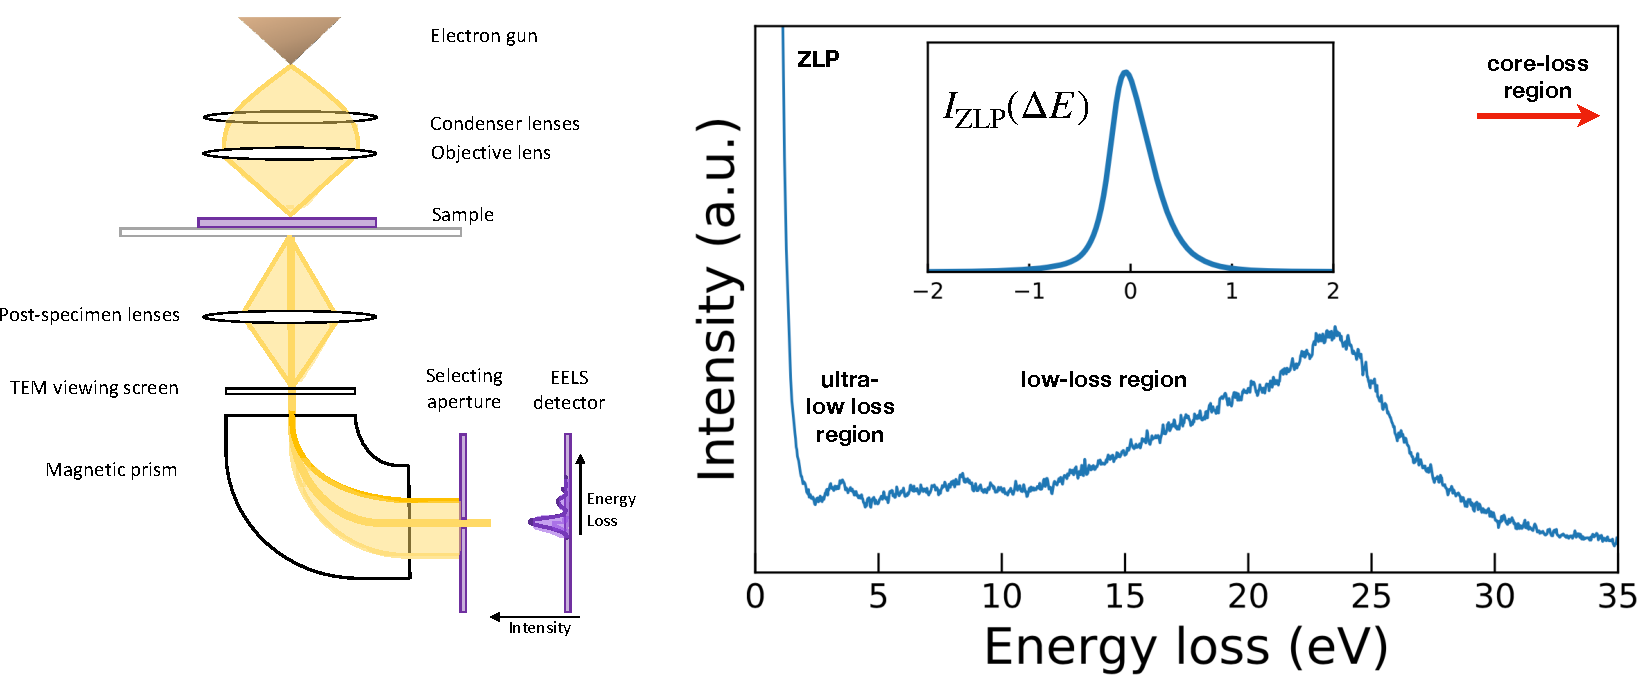
\includegraphics[width=0.9\textwidth]{plots/EELS.pdf}
    \caption{Left: in electron energy loss spectroscopy, a magnetic
      prism is used to deflect the electron beam that has crossed the sample
      in a way that the distribution of electron energy losses $\Delta E$ can be recorded
      by a spectrometer.
      Right: a representative EELS spectrum in the region $\Delta E \le 35$ eV, recorded
      on one of the WS$_2$ nanostructures presented~\cite{SabryaWS2}.
      %
      The inset displays the Zero Loss Peak, illustrating how
      its magnitude is larger than the contribution from the signal by several
      orders of magnitude.
      }
    \label{fig:EELS}
\end{figure}
%%%%%%%%%%%%%%%%%%%%%%%%%%%%%%%%%%%%%%%%%%%%%%%%5

The right panel of Fig.~\ref{fig:EELS} displays
a representative EELS spectrum in the region $\Delta E \le 35$ eV, recorded
on one of the WS$_2$ nanostructures presented~\cite{SabryaWS2}
and which will be further discussed in Sect.~\ref{sec:tmd}.
%
The inset displays the Zero Loss Peak, illustrating how
its magnitude is larger than the contribution from the inelastic scatterings
off the sample by several
orders of magnitude.
%
Clearly, carefully disentangling these two contributions in the region $\Delta E \simeq$ few eV
is essential for the physical interpretation of EEL spectra in the ultra-low-loss region.
%
The magnitude and shape of the ZLP intensity is known to depend not only on the specific values
of the electron energy loss $\Delta E$, but also in other operation parameters
of the TEM such as the electron beam energy $E_{\rm beam}$ and the exposure time
$T_{\rm exp}$, the aperture width and the use of a monochromator. 
%
This means that in general one cannot measure the ZLP for a given operation
conditions, say a high beam voltage of $E_{\rm b}=200$ keV, and expect to reproduce
the ZLP associated to different conditions, such as a  high beam voltage of $E_{\rm b}=60$ keV,
without introducing a specific model.
%
Several attempts to model the ZLP peak have had some success at fitting the main intensity of the peak, 
but in the tails discrepancies are as large as 25-35\%~\cite{Bangert:2003}. The standard background 
subtraction method is to fit a power law to the tails, however this subtraction is not suitable in
many circumstances and regimes~\cite{Hachtel:2018, Tenailleau:1992, Reed:2002, Bosman:2006}.
%
Unfortunately, it is not possible to compute the dependence of the ZLP on $\Delta E$
and the rest of operation parameters of the microscope from first principles.
%
Further, even for identical operation conditions the value of the ZLP
will in general vary due to {\it e.g.} external perturbations such as electric or magnetic fields~\cite{Rafferty:2000},
the stability of the microscope and spectrometer electronics~\cite{Kothleitner:2003}, the local
environment (possibly exposed to mechanical vibrations and pressure and temperature fluctuations) 
and spectral aberrations\cite{Egerton:1996, Scherzer:1949}. 
%

Any model for the ZLP should thus account for this irreducible source of uncertainties.
%
Several approaches to ZLP subtraction in EELS analyses have been suggested.
%
These are based on specific model assumptions about the ZLP properties, specifically
concerning its parametric functional dependence, from Lorentzian~\cite{Dorneich:1998}
and power laws~\cite{Erni:2005} to more general multiple-parameter functions~\cite{Benthem:2001}.
%
Another approach is based on the mirroring the $\Delta E <0$ region of the spectra, assuming
that the $\Delta E>0$ region is fully symmetric~\cite{Lazar:2003}.
%
These  subtraction methods are however affected by three main limitations.
%
Firstly, they rely on specific model assumptions {\it e.g.} with
the choice of functional form, introducing a methodological
bias whose size is difficult to quantify.
%
Secondly, they lack an estimate of the associated uncertainties, which in turn affects
the reliability of any physical interpretations of the low loss region such as the band gap extraction.
%
Thirdly, {\it ad hoc} choices of such as those of the fitting ranges introduce a significant degree of
arbitrariness in the procedure.
      
In this work we will investigate EELS measurements collected  on a cold field emission gun JEOL
transmission electron microscope operating at different beam energies $E_{\rm beam}$
and equipped with a  Gatan spectrometer.
%
The energy resolution is of these measurements,
defined as the FWHM of the ZLP, is $\delta E=40$ meV.
%
These measurements have a spatial resolution of ...

%%%%%%%%%%%%%%%%%%%%%%%%%%%%%%%%%%%%%%%%%%%%%%%%%%%%%%%%%%
%%%%%%%%%%%%%%%%%%%%%%%%%%%%%%%%%%%%%%%%%%%%%%%%%%%%%%%%%%


% Review of TMDs and WS2
\section{EELS analyses of TMDs nanostructures}
\label{sec:tmd}
\label{sec:eels}

In this work we apply our machine learning method to the study
of the low-loss EELS region for a specific type of WS$_2$ nanostructures known
as nanoflowers.
%
WS$_2$ is a transition metal dichalcogenide (TMD) material, which in turn
belongs to a class of materials known as two-dimensional, van der Waals, or simply layered materials.
%
These materials are
characterised by the remarkable property of being fully functional down to a single atomic layer.
%
In order to make the present study self-contained and accessible to a wider audience,
in this section we review the basic concepts underlying the EELS
method and discuss some of its recent applications to the study of TMDs nanostructures with emphasis
on WS$_2$.

\subsection{EELS and its ZLP in a nutshell}

Electron energy loss spectroscopy is a TEM-based method
whereby an electron-transparent sample is illuminated by a 
beam of energetic electrons.
%
Subsequently to the crossing of
the specimen, the scattered electron beam is focused by a magnetic prism
towards a spectrometer where the distribution of electron energy losses $\Delta E$ is recorded.
%
As schematic illustration of a typical EELS setup shown in the left panel of Fig.~\ref{fig:EELS}.
%
EEL spectra can be recorded either in the Scanning Transmission Electron Microscopy (STEM)
or in the conventional TEM modes.
%
Thanks to recent progress in TEM instrumentation and data acquisition, state-of-the-art EELS analyses befit from
a highly competitive energy (spectral) resolution combined with an unparalleled spatial resolution.

%%%%%%%%%%%%%%%%%%%%%%%%%%%%%%%%%%%%%%%%%%%%%%%
\begin{figure}[t]
    \centering
    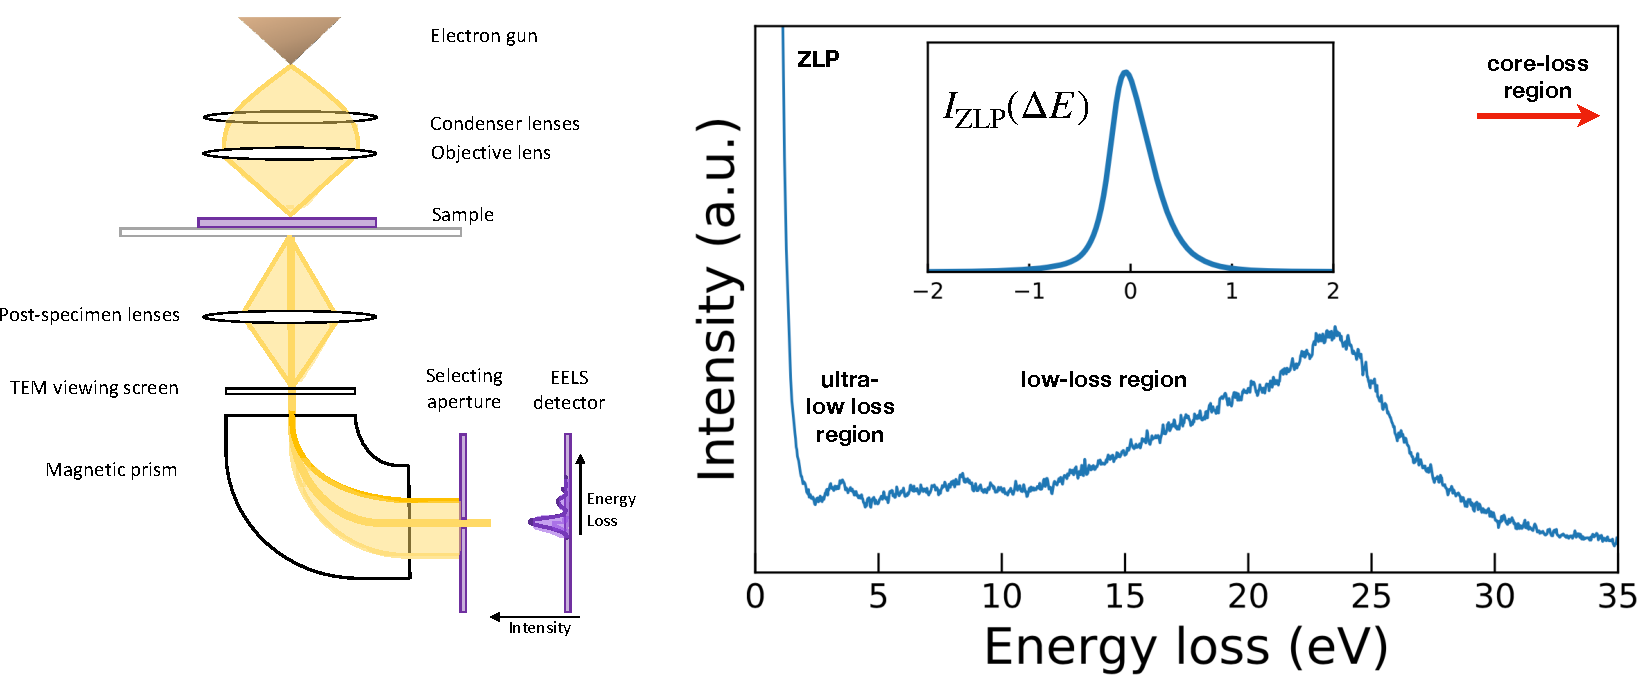
\includegraphics[width=0.9\textwidth]{plots/EELS.pdf}
    \caption{Left: in STEM-EELS, a magnetic
      prism is used to deflect the electron beam after crossing the sample
      so that the distribution of their energy losses $\Delta E$ can be recorded.
      %
      Right: a representative spectrum for $\Delta E \le 35$ eV acquired 
      on a WS$_2$ nanoflower~\cite{SabryaWS2} with
      the inset displaying the corresponding ZLP.
      }
    \label{fig:EELS}
\end{figure}
%%%%%%%%%%%%%%%%%%%%%%%%%%%%%%%%%%%%%%%%%%%%%%%%5

EELS spectra can be divided into three main regions.
%
The first one is the zero-loss region, centered around $\Delta E=0$
and that contains the contributions from both elastic scatterings
as well as those from electrons that have not interacted with the
sample.
%
This region is characterised by the strong, narrow ZLP which is there much larger than the contribution
from inelastic scatterings.
%
The second region is the low-loss region, defined for energy losses
$\Delta E \lsim 50$ eV and which contains information
about several important features such as plasmons, excitons, phonons, and
intra-band transitions.
%
Of particular relevance in this context is the ultra-low loss region, characterised by $\Delta E \simeq$ few eV
and where the contributions of the ZLP and that from the inelastic scatterings
off the sample are comparable.
%
For $\Delta E \gsim 50$ eV one then has the core-loss region,
which provides compositional information
on the materials that constitute the sample.
 
The right panel of Fig.~\ref{fig:EELS} displays
a representative EELS spectrum in the region $\Delta E \le 35$ eV, recorded
in one of the WS$_2$ nanostructures presented in~\cite{SabryaWS2}
and which will be further discussed below.
%
The inset displays the ZLP, illustrating how near $\Delta E\simeq 0$
its magnitude is larger than the contribution from the inelastic scatterings
off the sample by several
orders of magnitude.
%
Carefully disentangling these two contributions in the ultra-low-loss region
is essential for the physical interpretation of EEL spectra there.

The magnitude and shape of the ZLP intensity is known to depend not only on the specific values
of the electron energy loss $\Delta E$, but also in other operation parameters
of the TEM such as the electron beam energy $E_{\rm b}$, the exposure time
$t_{\rm exp}$, the aperture width, and whether or not a monochromator is being used. 
%
Since it is not possible to compute the dependence of the ZLP on $\Delta E$
and the other operation parameters of the microscope from first principles,
relying on specific models appears to be unavoidable.
%
This implies that one cannot measure the ZLP for a given operation
conditions, say a high beam voltage of $E_{\rm b}=200$ keV, and expect to reproduce
the ZLP distribution
associated to different conditions, such as a lower beam voltage of $E_{\rm b}=60$ keV,
without introducing model assumptions.

Several attempts to model the ZLP distribution have had some success at describing the main intensity of the peak, 
but in the tails discrepancies are as large as several tens of \%~\cite{Bangert:2003}.
%
The standard background 
subtraction method is to fit a power law to the tails, however this approach is not suitable in
many circumstances~\cite{Hachtel:2018, Tenailleau:1992, Reed:2002, Bosman:2006}.
%
Further, even for nominally identical operation conditions, the value of the ZLP
will in general vary due to {\it e.g.} external perturbations such as electric or magnetic fields~\cite{Rafferty:2000},
the stability of the microscope and spectrometer electronics~\cite{Kothleitner:2003}, the local
environment (possibly exposed to mechanical, pressure and temperature fluctuations) 
and spectral aberrations~\cite{Egerton:1996}. 
%
Any model for the ZLP should thus account for this irreducible source of uncertainties.


\subsection{TMD materials and WS$_2$ nanoflowers}

In this work we will apply, as a proof of concept, our machine-learning based method
for describing the ZLP to a novel class of WS$_2$ nanostructures known
as nanoflowers~\cite{SabryaWS2}.
%
WS$_2$ belongs to the TMD class of layered materials together with {\it e.g.}
MoS$_2$ and WSe$_2$.
%
TMD materials are of the form MX$_2$, where M is a 
transition metal atom (such as Mo or W) and X a chalcogen atom (such as S, Se, or Te). 
%
The characteristic crystalline structure of TMDs is such that
one layer of M atoms is sandwiched between two layers of X atoms.

The local electronic structure of TMDs strongly depends on the coordination 
between the transition metal atoms, giving rise to an array of remarkable electronic
and magnetic properties~\cite{Chhowalla:2013}.
%
Further, the properties of this class of materials vary quite significantly
with their thickness, for instance MoS$_2$ exhibits an indirect bandgap
in the bulk form which becomes direct at the monolayer level~\cite{Splendiani:2010}.
%
Such a tunable electronic structure and the potential applications in
nano-electronics makes TMD materials highly attractive for fundamental research. 

Here we are interested in studying specifically the local electronic
properties of WS$_2$ nanostructures.
%
As for other TMD materials, WS$_2$ adopts a layered structure 
by stacking atomic layers of S-W-S in a sandwich-like configuration. 
%
Although the interaction between adjacent layers is a weak Van der Waals 
force, the dependence of the interlayer interaction on the stacking 
order of WS$_2$ is significant.
%
Therefore, modulating the electronic
structure in a well-controlled way is crucial for application to
nano-devices.
%
WS$_2$  also exhibits a marked thickness dependence of
its properties, with an indirect-to-direct bandgap transition when going
from bulk to bilayer or monolayer form.
%
The effects of this transition are manifested as enhanced
photoluminescence in monolayer WS$_2$, whereas only little emission is observed in
the corresponding bulk form.
%
Further applications of this material include storage of hydrogen 
and lithium for batteries~\cite{Bhandavat:2012}.

%%%%%%%%%%%%%%%%%%%%%%%%%%%%%%%%%%%%%%%%%%%%%%%%%%%%%%%%%%%%%%%%%%%%%%%%%%%%%%%
\begin{figure}[t]
    \centering
    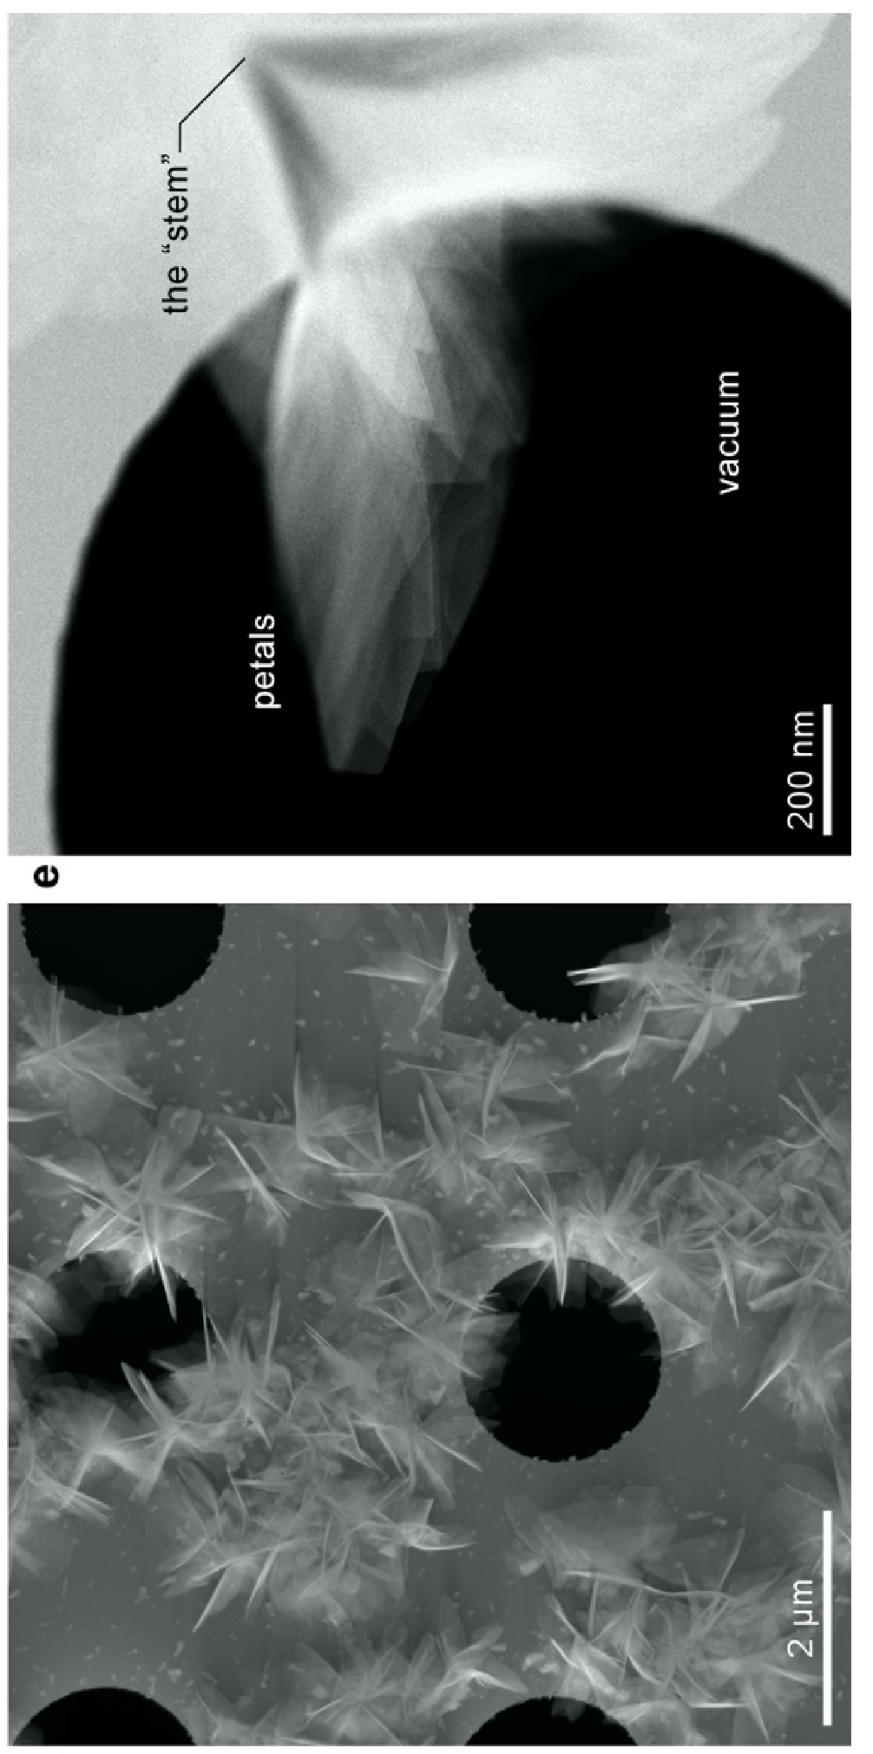
\includegraphics[width=0.49\textwidth,angle=-90]{plots/nanoflowers.pdf}
    \caption{Left: low-magnification TEM image of WS$_2$ nanoflowers
      grown on top of a holey TEM substrate. Right: a magnification of a
      representative {\it petals}
      of a flower and the {\it stem} that connects it to the substrate.
      %
      Note that the black region corresponds to the vacuum (no substrate).
      {\bf needs updating}
      }
    \label{fig:nanoflowers}
\end{figure}
%%%%%%%%%%%%%%%%%%%%%%%%%%%%%%%%%%%%%%%%%%%%%%%%%%%%%%%%%%%%%%%%%%%%%%%%%%%%%%%%%%5

A low-magnification TEM image of the WS$_2$ nanoflowers presented in~\cite{SabryaWS2} is displayed
in the left panel of Fig.~\ref{fig:nanoflowers}.
%
These nanostructures are grown directly in top of a holey TEM substrate.
%
In the right panel of the same figure we then show a magnification of a
      representative {\it petals}
      of a specific flower and the {\it stem} that connects it to the substrate.
      %
      Note that the black region corresponds to the vacuum, that is, without
      substrate underneath.
%
These WS$_2$ nanoflowers exhibit a wide variety of thicknesses, orientations,
and crystalline structures, therefore representing an ideal laboratory to correlate
structural morphology in WS$_2$ with electronic properties at the nanoscale.
%
Further, these nanoflowers display 3R/2H polytypism,
an important factor that determines the interlayer
interactions within WS$_2$: different stacking types tend to coexist, 
thus complicating the characterization of the physical properties~\cite{Na:2018}.
%
One consequence of the different stacking patterns is the appearance of
spontaneous electrical polarization, leading to modifications on the 
electronic band structure and correspondingly on the band gap~\cite{Lee:2016}.

As mentioned above, one of the most interesting properties of  WS$_2$ is
that when the material
is thinned down to a single monolayer, its indirect band gap of
$E_{\rm bg}\simeq 1.4$ eV
switches to a direct band gap of approximately $E_{\rm bg}\simeq 2.1$ eV.
%
In general, it has been found that the type and magnitude of the bandgap
of WS$_2$ depends quite sensitively on the crystalline structure and
the number of layers that constitute the material.
%
In Table~\ref{table:bgvalues} we collect
representative results for the determination of the bandgap energy $E_{\rm bg}$
and its type in WS$_2$, obtained by means of different experimental and theoretical techniques.
%
 For each reference we indicate separately the bulk results and those
obtained at the monolayer (ML) level.
%
We note that at the monolayer level there is a fair spread of results in the
value of $E_{\rm bg}$, reflecting the challenges of its accurate determination.
 
%%%%%%%%%%%%%%%%%%%%%%%%%%%%%%%%%%%%%%%%%%%%%%%%%%%%%%%%%%%%%%%%%%%%%%%%%%%%%%%%%%%%%
\begin{table}[t]
  \small
  \begin{centering}
   \renewcommand{\arraystretch}{1.20}
\begin{tabular}{ccccc}
\br
Reference                       & Thickness & $E_{\rm bg}$ (eV)  & Band gap type  & Technique \\
\mr
{\cite{Braga:2012}} & bulk   & $1.4\pm0.07$            & indirect  & {Gate-voltage dependence}  \\
\mr
\multirow{2}{*}{\cite{Jo:2014}}                 & ML   & $2.14 $         & direct  & \multirow{2}{*}{Gate-voltage dependence}        \\
& bulk & $1.40 $    & indirect              \\
\mr

\multirow{2}{*}{\cite{Gusakova:2007}} & ML   & $2.03\pm0.03$            & direct  & \multirow{2}{*}{DFT}  \\
& bulk & $1.32\pm0.03 $            & indirect     \\
\mr
\multirow{2}{*}{\cite{Kam:1982}}                  & ML   & $1.76\pm0.03 $      & direct    & \multirow{2}{*}{Absorption edge coefficient fitting}         \\
& bulk & $1.35 $          & indirect        \\
\mr
\cite{Shi:2013}                & ML   & $2.21\pm0.3 $         & direct  & Bethe-Salpeter equation (BSE)        \\                 \br                                         
\end{tabular}
\vspace{0.27cm}
\caption{Representative results for the determination of the bandgap energy $E_{\rm bg}$
  and its type in WS$_2$, obtained by means of different experimental and theoretical techniques.
  %
  For each reference we indicate separately the bulk results and those
  obtained at the monolayer (ML) level.}
    \label{table:bgvalues}
    \end{centering}
\end{table}
%%%%%%%%%%%%%%%%%%%%%%%%%%%%%%%%%%%%%%%%%%%%%%%%%%%%%%%%%%%%%%%%%%%%%%%%%%%%%%%%%%%%%%


% Discuss the methodology that we are going to use
%%%%%%%%%%%%%%%%%%%%%%%%%%%%%%%%%%%%%%%%%%%%%%%%%%%%%%
\section{Neural network determination of the ZLP}
%%%%%%%%%%%%%%%%%%%%%%%%%%%%%%%%%%%%%%%%%%%%%%%%%%%%%
\label{sec:methodology}

In this section we present our strategy to parametrise and subtract in a model-independent manner
the zero-loss peak that arises in the low-loss region of EEL spectra by means
of machine learning.
%
As mentioned in the introduction, our strategy will be inspired by the 
NNPDF method~\cite{Rojo:2018qdd} originally developed in the context of high-energy physics
for studies of the quark and gluon substructure of the proton~\cite{Gao:2017yyd}.
%
The NNPDF approach has been successfully applied, among others, to
the determination of
unpolarised~\cite{DelDebbio:2007ee,Ball:2008by,Ball:2012cx,Ball:2014uwa,Ball:2017nwa}
and polarised parton distributions functions of protons,  nuclear
parton distributions~\cite{AbdulKhalek:2019mzd,AbdulKhalek:2020yuc}, and the
fragmentation functions of partons into neutral and charged
hadrons~\cite{Bertone:2017tyb,Bertone:2018ecm}.

We note that recently several applications of machine learning
to transmission electron microscopy analyses 
in the context of material science have been
presented, see {\it e.g.}~\cite{Gordon:2020, Zhang:2019, Jany:2017, Ziatdinov:2017,10.1145/2834892.2834896,doi:10.1021/acsnano.7b07504,cite-key}.
%
Representative examples
include the automated identification
of atomic-level structural information~\cite{10.1145/2834892.2834896},
the extraction of chemical information
and defect classification~\cite{doi:10.1021/acsnano.7b07504},
and spatial resolution enhancement
using  using a generative adversarial network~\cite{cite-key}.
%
To the best of our knowledge, this is
the first time that neural networks are used as 
 unbiased
 background-removal interpolators
 and combined with Monte Carlo sampling to construct a faithful estimate
of the model uncertainties.

In this section
first of all we discuss the parametrisation of the ZLP in terms of neural networks.
%
We then review the Monte Carlo replica method used to estimate and propagate the
uncertainties to the input data to the model predictions.
%
Subsequently, we present our training strategy both in case of vacuum and of sample spectra,
and discuss how one can select the hyper-parameters that appear in the model.

\subsection{ZLP parametrisation}
\label{sec:parametrisation}

To begin with we note that, without any loss of generality, the intensity profile
associated to an EEL spectrum may be decomposed as
\be
\label{eq:IeelTot}
I_{\rm EEL}(\Delta E) =I_{\rm ZLP}(\Delta E) + I_{\rm inel}(\Delta E) \, ,
\ee
where $\Delta E$ is the measured electron energy loss; $I_{\rm ZLP}$ is the zero-loss peak
distribution arising both from instrumental origin  and from elastic scatterings; and
$I_{\rm inel}(\Delta E)$ contains the contributions from the
inelastic scatterings off the electrons and atoms in the specimen.
%
As shown by the representative example of Fig.~\ref{fig:EELS}, there are two limits
for which one can cleanly disentangle the two contributions.
%
First of all, for large enough values of
$\Delta E$ then
$I_{\rm ZLP}$ vanishes and thus $I_{\rm EEL} \to I_{\rm inel}$.
%
Secondly, in the $\Delta E\simeq 0$ limit all emission can be associated to
 the ZLP such that $I_{\rm EEL}\to  I_{\rm ZLP}$.
%
In this work we are interested in the ultra-low-loss region, where $I_{\rm ZLP}$ and $I_{\rm inel}$
become of the comparable magnitude.

Our goal is to construct a parametrisation of $I_{\rm ZLP}$ based on artificial
neural networks, which we denote by $I_{\rm ZLP}^{\rm (mod)}$, whereby we
can extract the relevant inelastic contribution by subtracting the
ZLP background to the measured intensity spectra,
\be
\label{eq:ZLPseparation}
I_{\rm inel}(\Delta E) \simeq I_{\rm EEL}(\Delta E) - I_{\rm ZLP}^{\rm (mod)}(\Delta E) \, ,
\ee
and thus be able to exploit the physical information contained in $I_{\rm inel}$ in
the low-loss region.
%
Crucially, we aim to faithfully estimate and propagate all the relevant sources of uncertainty associated
both to the input data and to methodological choices.

As discussed in Sect.~\ref{sec:eels}, the ZLP depends both
on the value of the electron energy loss $\Delta E$ as well as on the operation
parameters of the microscope, such as the electron beam energy $E_b$ and the exposure time
$t_{\rm exp}$.
%
Therefore we want to construct a multidimensional model which takes all relevant
variables as input.
%
This means that in general Eq.~(\ref{eq:ZLPseparation}) must be written as
\be
I_{\rm inel}(\Delta E) = I_{\rm EEL}(\Delta E, E_{b},t_{\rm exp}, \ldots) - I_{\rm ZLP}^{\rm (mod)}(\Delta E, E_{b},t_{\rm exp}, \ldots) \, ,
\ee
where we note that the subtracted spectra should depend only on $\Delta E$ but not on the microscope
operation parameters.
%
Ideally, the ZLP model should be able to accomodate as many input variables as possible.
%
Here we parametrise $I_{\rm ZLP}^{\rm (mod)}$ by means of
multi-layer feed-forward artificial neural networks, that is, we express our ZLP model as
\be
\label{eq:ZLPmodelNN}
I_{\rm ZLP}^{\rm (mod)}(\Delta E, E_{b},t_{\rm exp}, \ldots)  = \xi^{(n_l)}_1(\Delta E, E_{b},t_{\rm exp}, \ldots) \, ,
\ee
where $\xi^{(n_l)}_1$ denotes the activation state of the single neuron in the last
of the $n_l$ layers of the network when the $n_I$ inputs $\{ \Delta E, E_{b},t_{\rm exp}, \ldots \}$
are used.
%
The weights and thresholds of this neural network model are then determined
from the maximization of the model likelihood by means
of supervised learning and non-linear regression from a suitable training dataset.
%
This type of neural networks benefit from the ability
to parametrise multidimensional input data with arbitrarily
non-linear dependencies: even with a single hidden layer, a neural network
can reproduce arbitrary functional dependencies provided it has a large enough
number of neurons.

A schematic representation of our model
is displayed in Fig.~\ref{fig:architecture}.
%
 The input is an $n_I$ array containing $\Delta E$ and the rest of
 operation variables of the microscope, and
 the output is the value of the intensity of the ZLP distribution
 associated to those input variables.
 %
 We adopt an $n_I$-10-15-5-1 architecture with three hidden layers, for a total
 number of 289~(271) free parameters for $n_I=3$~($n_I=1$) to be adjusted by the optimization procedure.
 %
 We use a sigmoid activation function for the three hidden layers and a ReLU
 for the final one.
 %
 The choice of ReLU for the final layer guarantees that our model for the ZLP
 is positive-definite, as required by general physical considerations.
 %
 We have adopted a redundant architecture  to ensure that the ZLP parametrisation
 is sufficiently flexible, and we avoid over-fitting by means of
 a suitable regularisation strategy, see Sect.~\ref{sec:training}.
  
%%%%%%%%%%%%%%%%%%%%%%%%%%%%%%%%%%%%%%%%%%%%%
\begin{figure}[t]
    \centering
    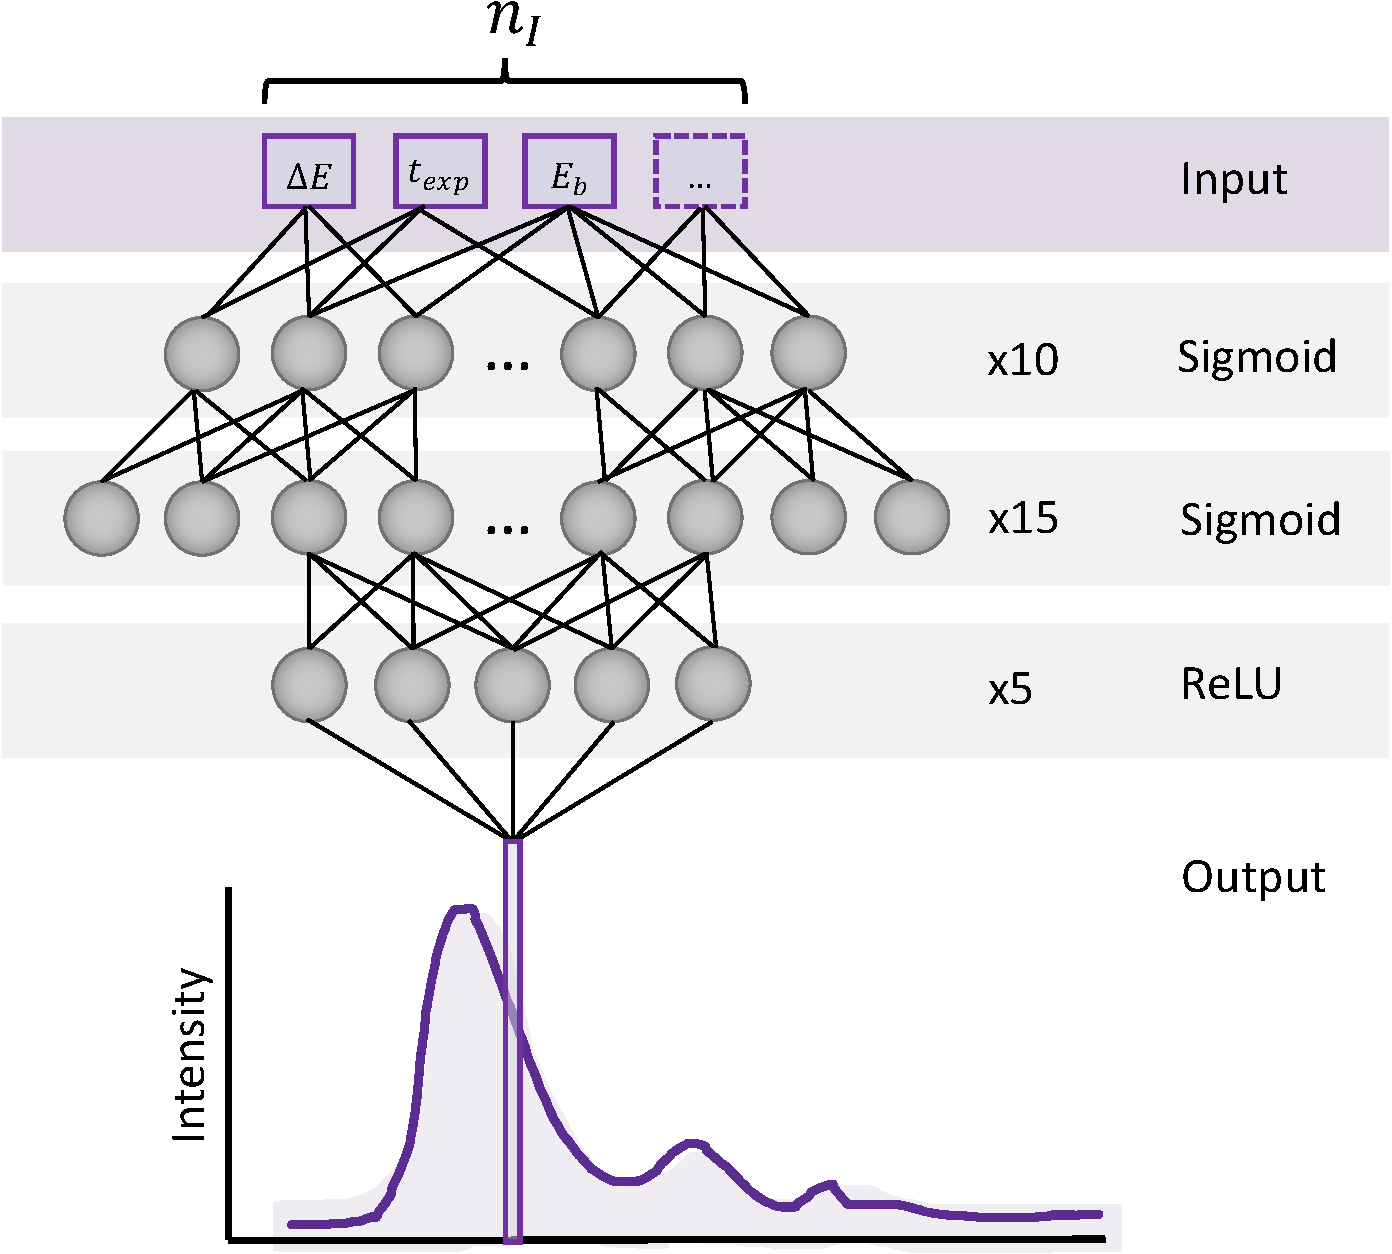
\includegraphics[width=99mm]{plots/architecture.pdf}
    \caption{Schematic representation of our ML model for the ZLP, Eq.~(\ref{eq:ZLPmodelNN}).
      %
      The input is an $n_I$-dimensional array containing $\Delta E$ and other
      operation variables of the microscope such as $E_b$ and $t_{\rm exp}$.
      %
      The output is the predicted value of the intensity of the zero-loss peak
      distribution associated to those specific input variables.
      %
      The architecture is chosen to be $n_I$-10-15-5-1, with sigmoid activation functions
      in all layers except for a ReLU in the output neuron.
    }
    \label{fig:architecture}
\end{figure}
%%%%%%%%%%%%%%%%%%%%%%%%%%%%%%%%%%%%%%%%%%%%%%%%%

\subsection{Uncertainty propagation}

We discussed in Sect.~\ref{sec:eels} how
even for EEL spectra taken at identical operation conditions of the microscope,
in general the resulting ZLP intensities will differ.
%
Further, there exist a large number of different NN configurations, each
representing a different functional form for $I_{\rm ZLP}^{(\rm mod)}$ which provide
an equally valid description of the input data.
%
To  estimate these uncertainties and propagate them to physical predictions,
we use here the Monte Carlo replica method.
%
The basic idea  is to exploit the available information
on experimental measurements (central values, uncertainties, and correlations)
to construct a sampling of the probability density in the space of 
the data, which by means of the NN training is then propagated
to a probability density in the space of $I_{\rm ZLP}$ models.

Let us assume that we have $n_{\rm dat}$ independent measurements of the ZLP intensity, for
different or the same values of the input parameters collectively denoted as $\{z_i\}$:
\be
I^{\rm (exp)}_{{\rm ZLP},i}\lp \{ z_i  \}\rp = I^{\rm (exp)}_{{\rm ZLP},i}\lp  \Delta E_i, E_{b,i}, t_{\rm exp,i},\ldots \rp
\,, \quad i=1,\ldots,n_{\rm dat} \, .
\ee
The Monte Carlo method is based on the generation
of a large number $N_{\rm rep}$ of Monte Carlo replicas of these original data points
by means of a multi-Gaussian distribution, with the central values and covariance matrices
from the input measurements,
\be
\label{eq:MCreplicaGen}
  I_{{\rm ZLP},i}^{{\rm (art)}(k)}  =  I^{\rm (exp)}_{{\rm ZLP},i} + r_i^{({\rm stat},k)}\sigma_i^{\rm (stat)}
  + \sum_{j=1}^{n_{\rm sys}} r_{i,j}^{({\rm sys},k)} \sigma_{i,j}^{\rm (\rm sys)} \,, \quad \forall i
  \,, \quad k=1,\ldots,N_{\rm rep} \,.\,\, \,
  \ee
  where $\sigma_i^{\rm (stat)}$ and $\sigma_{i,j}^{\rm (\rm sys)}$ represent the statistical
  and systematic uncertainties (the latter divided into  $n_{\rm sys}$ fully point-to-point correlated
  sources) and $\{r_i^{(k)}\}$ are Gaussianly distributed random numbers.
  %
  The values of $\{r_i^{(k)}\}$ are
  generated with a suitable correlation pattern to ensure
  that averages over the set of Monte Carlo
  replicas reproduce the original experimental covariance matrix, namely
  \be
  \la  \lp I_{{\rm ZLP},i}^{{\rm (art)}(k)} - \la I_{{\rm ZLP},i}^{{\rm (art)}}\ra_{\rm rep}\rp
  \lp I_{{\rm ZLP},j}^{{\rm (art)}(k)} - \la I_{{\rm ZLP},j}^{{\rm (art)}}\ra_{\rm rep}\rp\ra_{\rm rep}
  \label{eq:expcovariance} = {\rm cov}^{(\rm exp)}\lp I_{{\rm ZLP},i},I_{{\rm ZLP},j}\rp  \, ,
  \ee
  where averages are evaluated over the $N_{\rm rep}$ replicas that compose the sample.
  %
We thus note that each $k$-th replica contains 
as many data points as the original set.

In our case the information on experimental correlations is not accessible and
thus we assume that there is a single source of point-by-point uncorrelated systematic
uncertainty, denoted as $\sigma_i^{\rm (exp)}$, which is estimated as follows.
%
The input measurements will be composed in general on subsets of EEL
spectra taken with identical operation conditions.
%
Assume that for a specific set of operation conditions we have $N_{\rm sp}$ of such spectra.
%
Since the values of $\Delta E$ will be different in each case, first of all
we uniformise a common binning in $\Delta E$ with $n_{\rm dat}$ entries.
%
Then we evaluate the total experimental uncertainty in one of these bins as
\be
\label{eq:sigmaiexp}
\sigma_i^{\rm (exp)} = \lp \frac{1}{N_{\rm sp}-1} \sum_{l=1}^{N_{\rm sp}}
\lp I_{{\rm ZLP},i}^{ ({\rm exp}),l}  - \la I_{{\rm ZLP},i}^{ ({\rm exp})}\ra_{N_{\rm sp}} \rp \rp^{1/2} \, ,\,
i=1,\ldots, n_{\rm dat} \, ,
\ee
that is, as the standard deviation over the $N_{\rm sp}$ spectra.
%
This uncertainty is separately evaluated for each set of microscope operation conditions
for which data available.
%
In the absence of correlations Eqns.~(\ref{eq:MCreplicaGen}) and~(\ref{eq:expcovariance}) thus
simplify to
\be
 I_{{\rm ZLP},i}^{{\rm (art)}(k)}  =  I^{\rm (exp)}_{{\rm ZLP},i} + r_i^{({\rm tot},k)}\sigma_i^{\rm (exp)}
 \,, \quad \forall i
  \,, \quad k=1,\ldots,N_{\rm rep} \,.\,\, \,
\ee
and
  \bea
  \la  \lp I_{{\rm ZLP},i}^{{\rm (art)}(k)} - \la I_{{\rm ZLP},i}^{{\rm (art)}}\ra_{\rm rep}\rp
  \lp I_{{\rm ZLP},j}^{{\rm (art)}(k)} - \la I_{{\rm ZLP},j}^{{\rm (art)}}\ra_{\rep}\rp\ra_{\rm rep} =
  \sigma_i^{\rm (exp)}\sigma_j^{\rm (exp)}\delta_{ij} \, ,
  \eea
  given that the experimental covariance matrix is diagonal.
  %
  Should in the future correlations became available, it would be straightforward to extend
  our model to that case.

The value of the number of generated MC replicas, $N_{\rm rep}$, should be chosen such that the set of replicas 
models accurately the probability distribution of original training data.
%
To verify that this is the case,
Fig.~\ref{fig:MC} displays a comparison between the original experimental central values
$I_{{\rm ZLP},i}^{\rm (exp)}$ (left) and the corresponding 
total uncertainties $\sigma_i^{(\rm exp)}$ (right panel) with the results of averaging over
a sample of $N_{\rm rep}$ Monte Carlo replicas generated by means of
Eq.~(\ref{eq:MCreplicaGen}) for different number of replicas.
%
We find that $N_{\rm rep}=500$ is a value that ensures that both
the central values and uncertainties are reasonably well reproduced,
and we adopt it in what follows.

%%%%%%%%%%%%%%%%%%%%%%%%%%%%%%%%%%%%%%%%%%%%%%%
\begin{figure}[t]
    \centering
    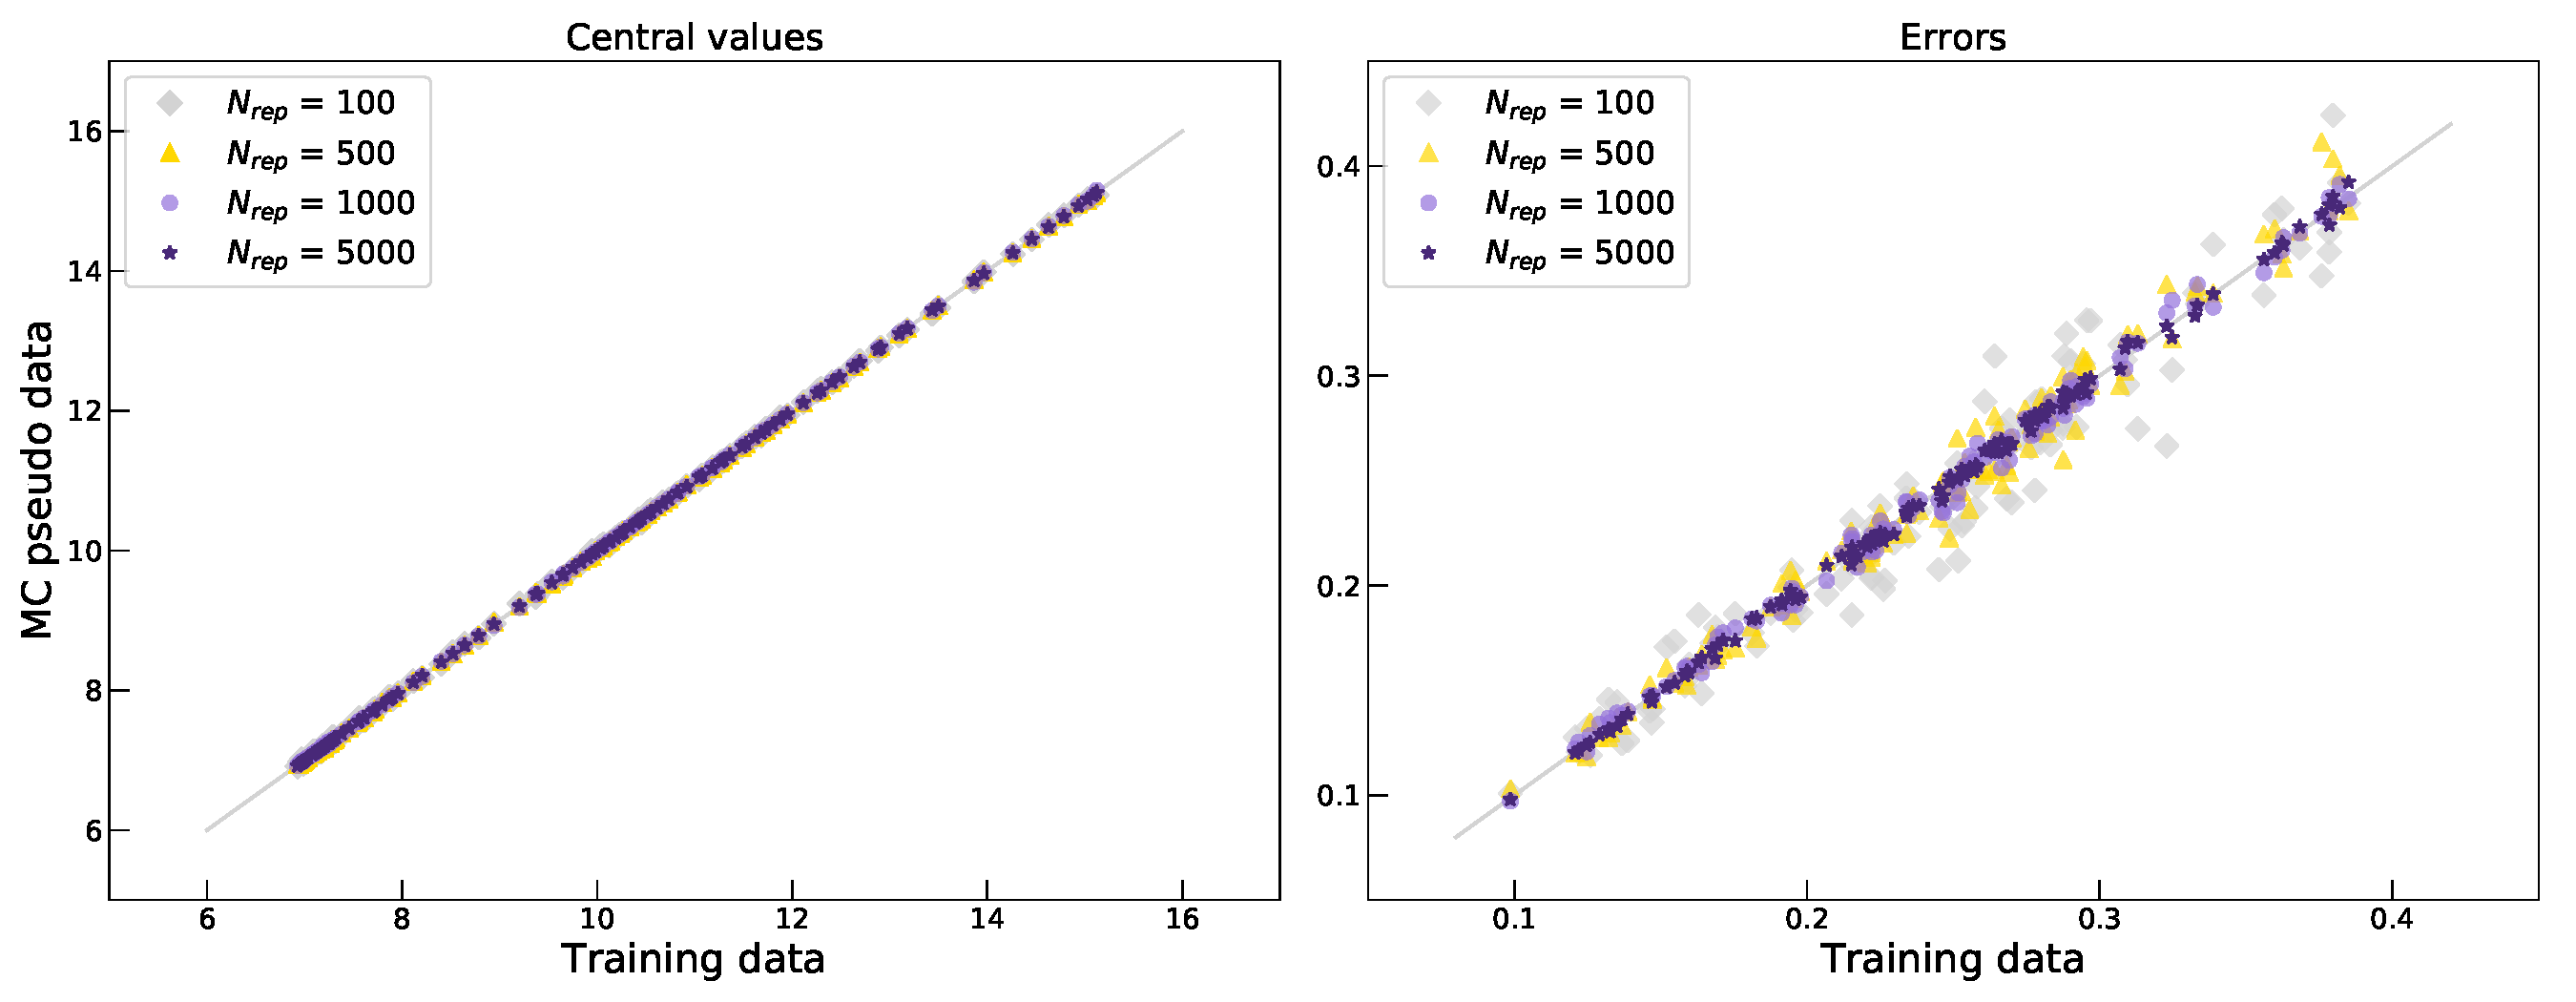
\includegraphics[width=0.99\textwidth]{plots/MC.pdf}
    \caption{Comparison between the original experimental central values
      $I_{\rm ZLP,i}^{\rm exp}$ (left panel) and the corresponding statistical
      uncertainties $\sigma_i^{(\rm stat)}$ with the results of averaging over
      a sample of $N_{\rm rep}$ Monte Carlo replicas generated by means of
      Eq.~(\ref{eq:MCreplicaGen}), for different values of
      $N_{\rm rep}$.
      }
    \label{fig:MC}
\end{figure}
%%%%%%%%%%%%%%%%%%%%%%%%%%%%%%%%%%%%%%%%%%%%%%%%5

\subsection{Training strategy}
\label{sec:training}

The training of the neural-network model for the ZLP peak differs between
the cases of EEL spectra taken on vacuum, where by construction $I_{\rm EEL}(\Delta E) =I_{\rm ZLP}^{\rm (mod)}(\Delta E)$,
and for spectra taken on sample.\footnote{Actually EEL spectra taken in the vacuum but close
  to the sample might still receive inelastic contributions due to processes such as .... Here
  when we use vacuum spectra we consider exclusively those taken reasonably far from the surface
of the analysed nanostructures.}
%
In the latter case, as indicated by Eq.~(\ref{eq:ZLPseparation}), in order to avoid
biasing the results it is
important to ensure that the model is trained only on the region of the spectra
where the ZLP dominates over the inelastic scatterings.
%
We now describe the training strategy that is adopted in both cases.

\paragraph{Training of vacuum spectra.}
%
For each of the $N_{\rm rep}$ generated Monte Carlo replicas, we train an independent
neural network as described in Sect.~\ref{sec:parametrisation}.
%
The parameters of the neural network are determined from the minimisation of a figure of merit
defined as
\begin{equation}
  \label{eq:chi2}
\begin{centering}
  E^{(k)}\lp \{\theta^{(k)}\}\rp = \frac{1}{n_{\rm dat}}\sum_{i=1}^{n_{dat}}\left(\frac{ I_{{\rm ZLP},i}^{{\rm (art)}(k)} -
  I_{{\rm ZLP},i}^{{\rm (mod)}}\lp \{\theta^{(k)}\}\rp }{\sigma_i^{(\rm exp)}}\right)^2, 
\end{centering}
\end{equation}
which is the $\chi^2$ per data point comparing the $k$-th replica for the ZLP
intensity with the corresponding model prediction for the values
$\{\theta^{(k)}\}$ of its weights and thresholds.
%
In order to speed up the neural network training process, prior to the optimisation
all inputs and outputs are scaled to lie between $[0.1, 0.9]$ before
being feed to the network.
%
This preprocessing facilitates that
 the neuron activation states will typically
lie close to the linear region of the sigmoid activation function.

The contribution to the figure of merit from the input experimental data, Eq.~(\ref{eq:chi2}),
needs in general to be complemented with that of theoretical constraints on the model.
%
For instance, when determining nuclear parton distributions~\cite{AbdulKhalek:2020yuc}, one needs to
extend Eq.~(\ref{eq:chi2}) with Lagrange multipliers to ensure that both the $A=1$ proton boundary
condition and the cross-section positivity are satisfied.
%
In the case at hand, our model for the ZLP should implement the property that $I_{\rm ZLP}(\Delta E)\to 0$
when $|\Delta E| \to \infty$, since far from $\Delta E\simeq 0$ the contribution from elastic scatterings
and instrumental broadening is completely negligible.
%
In order to implement this constraint, we add $n_{pd}$ pseudo-data points to the training dataset and modify
the figure of merit Eq.~(\ref{eq:chi2}) as follows
\be
\label{eq:chi2modified}
E^{(k)}\lp \{\theta^{(k)}\}\rp \to E^{(k)}\lp \{\theta^{(k)}\}\rp +
\lambda \sum_{i'=1}^{n_{pd}}\left(
  I_{{\rm ZLP},i'}^{{\rm (mod)}}\lp \{\theta^{(k)}\}\rp \right)^2, 
  \ee
  where $\lambda$ is a Lagrange multiplier whose value is tuned to ensure that the $I_{\rm ZLP}(\Delta E)\to 0$
  condition
  is satisfied without affecting the description of the training dataset.
  %
  The pseudo-data points are chosen to lie in the region $\lc \Delta E_{\rm pd}^{\rm (min)},
  \Delta E_{\rm pd}^{\rm (max)}\rc$ (and symmetrically for negative energy losses),
  which is determined automatically via the ratio of the intensity to the uncertainty in each data point: 
  $I_{ZLP,i}^{(exp)} / \sigma_{i}^{(exp)}$. 
  %
  At a certain energy loss this ratio approaches 1, which indicates that we are practically fitting noise. 
  %
  In order to avoid this and only fit data that is different from zero within errors, we set the value
  of $\Delta E_{\rm pd}^{\rm (min)}$ for each set of training data equal to the point where the ratio
  $I_{ZLP,i}^{(exp)} / \sigma_{i}^{(exp)}$ drops below 1. 
  %
  We keep the training data in the region $\Delta E \le \Delta E_{\rm pd}^{\rm (min)}$ and the pseudo-data
  points are added for $\lc \Delta E_{\rm pd}^{\rm (min)}, \Delta E_{\rm pd}^{\rm (max)}\rc$. 
  %
  The value of $\Delta E_{\rm pd}^{\rm (max)}$ can be chosen arbitrarily and can be as large as necessary
  to ensure that $I_{\rm ZLP}(\Delta E)\to 0$ as $|\Delta E| \to \infty$.
  %u
We note that another important physical condition on the ZLP model, namely its positivity
(since in EEL spectra the intensity is just a measure of the number of counts in the
detector for a given value of the energy loss) is automatically satisfied since
we use a ReLU activation function for the last layer.

In this work we adopt the {\tt TensorFlow} neural-net libraries to assemble
the architecture illustrated in  Fig.~\ref{fig:architecture}.
%
Before training, all weights and biases are initialized in a non-deterministic order
by the built-in global variable initializer. 
%
The optimisation of the figure of merit Eq.~(\ref{eq:chi2modified}) is carried
out by means of stochastic gradient descent combined with backpropagation,
in particular by means of the Adam algorithm.
%
The hyper-parameters of the optimisation algorithm such as the learning rate
have been adjusted to ensure proper learning is reached in the shortest amount
of time possible.
%

Given that we have a extremely flexible parametrisation, one should be careful
to avoid overlearning the input data.
%
Here over-fitting is avoided by means of a cross-validation stopping criterion.
%
We separate the input data into training a validation subsets, with a 80\%/20\% splitting
which varies randomly for each Monte Carlo replica.
%
We then run the optimiser for a very large number of iterations and store both
the state of the network and the value
of the figure of merit Eq.~(\ref{eq:chi2}) restricted to the validation
dataset, $E^{(k)}_{\rm val}$ (which is not used for the training).
%
The optimal stopping point is then determined {\it a posteriori} for each replica
as the specific network configuration that leads to the deepest minimum of $E^{(k)}_{\rm val}$.
%
The number of epochs should be chosen high enough to reach the optimal stopping point for each replica.
For this work we need approximately 40,000 epochs to ensure overlearning.
%
This corresponds to a running time of 60 seconds per replica when training on a set of 500 datapoints.
%
Once the training of all the $N_{\rm rep}$ neural network models for the ZLP has been carried
out as specified above, we gauge the overal fit quality of the model by computing the
$\chi^2$ defined as
\begin{equation}
  \label{eq:chi2_final}
\begin{centering}
  \chi^2 = \frac{1}{n_{\rm dat}}\sum_{i=1}^{n_{dat}}\left(\frac{ I_{{\rm ZLP},i}^{{\rm (exp)}} -
 \la I_{{\rm ZLP},i}^{{\rm (mod)}}\ra_{\rm rep} }{\sigma_i^{(\rm exp)}}\right)^2, 
\end{centering}
\end{equation}
which is the analog of Eq.~(\ref{eq:chi2_final}) now comparing the average model prediction
to the original experimental data values.
%
A value $\chi^2 \simeq 1$ indicates that a satisfactory description of the experimental data,
within the corresponding uncertainties, has been achieved.
%
Note that in realistic scenarios $\chi^2$ can deviate from unity, for instance when
some source of correlation between the experimental uncertainties has been neglected.

\paragraph{Training of sample spectra.}

The training strategy in the case of EEL spectra taken on samples (rather than on vacuum) must be adjusted
to account for the fact that the input data set, Eq.~(\ref{eq:IeelTot}), receives contributions
both from the ZLP and from inelastic scatterings.
%
To avoid biasing the ZLP model, only the former contributions should be
included in the training dataset.

We can illustrate the situation here with the help of a toy model for the low-loss
region of EEL spectra, represented in
Fig.~\ref{fig:EELS_toy}.
%
Let us assume that the ZLP is described by a Gaussian distribution with a standard deviation of $\sigma_{\rm ZLP}=0.3$ eV,
and that the contribution from the
inelastic scatterings arising from the sample can be approximated in the low-loss
region by $I_{\rm inel}(\Delta E)\propto \lp \Delta E - E_{\rm bg}\rp^b$ with $E_{\rm bg}=1.5$
and $b=0.5$ -- the motivation for this
choice will be spelled out in Sect.~\ref{sec:results_sample}.
%
We display the separate contributions from $I_{\rm ZLP}$
and $I_{\rm inel}$, as well as their sum, 
with the inset showing the values of the corresponding derivatives, $dI/d\Delta E$.

%%%%%%%%%%%%%%%%%%%%%%%%%%%%%%%%%%%%%%%%%%%%%
\begin{figure}[t]
    \centering
    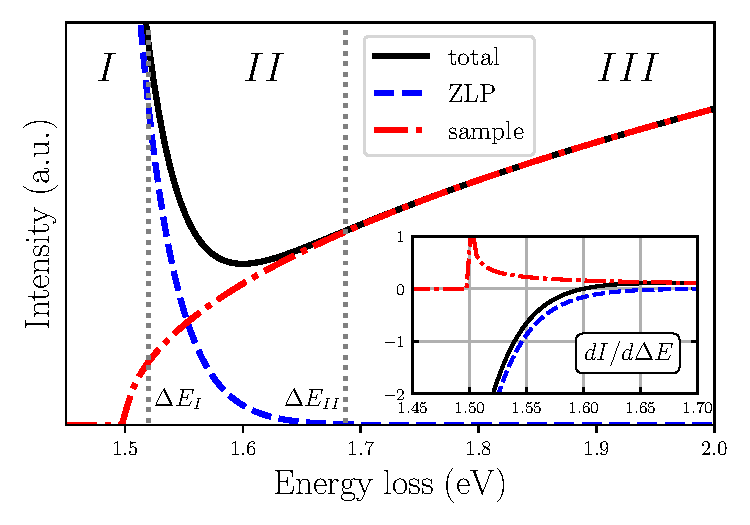
\includegraphics[width=0.89\textwidth]{plots/EELS_toy.pdf}
    \caption{A toy model for the EEL spectrum and its
      derivative (in the inset).
      %
      We display the separate contributions from $I_{\rm ZLP}$
      and $I_{\rm inel}$ as well as their sum.
      %
      We indicate the two regions used for the model training ($I$ and $III$),
      while as discussed in the text the trained model is then
      extrapolated to region $II$, defined for $\Delta E_I \le \Delta E \le \Delta E_{II}$.
    }
    \label{fig:EELS_toy}
\end{figure}
%%%%%%%%%%%%%%%%%%%%%%%%%%%%%%%%%%%%%%%%%%%%%%%%%

The toy model of Fig.~\ref{fig:EELS_toy} is general enough so that one can draw
a number of useful considerations concerning the relation between $I_{\rm ZLP}$ and $I_{\rm inel}$
in realistic spectra:

\begin{itemize}

\item The ZLP intensity, $I_{\rm ZLP}(\Delta E)$, is a monotonically decreasing function
  and thus its derivative is always negative.

\item  The first local minimum of the total spectrum, $dI_{\rm EELS}/d\Delta E|_{\Delta E_{\rm min}}=0$, corresponds
  to a value of $\Delta E$ for which the contribution from the inelastic emissions is already
  sizable.

\item The value of $\Delta E$ for which $I_{\rm inel}$ starts to contribute to the total spectrum
  corresponds to the position where the intensity derivatives in-sample and in-vacuum  start to differ.
  %
  We note that a direct comparison between the overal magnitude of the sample and vacuum ZLP
  spectra is in general not possible, as explained in Sect.~\ref{sec:eels}. 
\end{itemize}

These considerations suggest that when training the ML model on EEL spectra taken on samples,
the following categorisation should de adopted:

\begin{enumerate}

\item For energy losses such that $\Delta E \le \Delta E_I$ (region $I$),
  the model training  proceeds in the same way as for the vacuum case
  via the minimisation of Eq.~(\ref{eq:chi2})

\item  
  For $\Delta E \ge \Delta E_{II}$ (region $III$), we use instead Eq.~(\ref{eq:chi2modified})
  without the contribution from the input data, since for such values
  of $\Delta E$ one has that $I_{\rm inel}\gg I_{\rm ZLP}$.
  %
  In other words, the only information that the region $III$ provides
  on the model is the one arising from the implementation
  of the constraint that $I_{\rm ZLP}(\Delta E\to \infty)\to 0$.

\item The EELS data  in region $II$, defined by  $\Delta E_I \le \Delta E \le \Delta E_{II}$,
  is excluded from the training dataset, given that in this region the contribution to $I_{\rm EEL}$
  coming from $I_{\rm inel}$ is significant.
  %
  There the model predictions are obtained from an interpolation
  of the predictions obtained in regions $I$ and $III$.

\end{enumerate}

This classification introduces two new hyper-parameters of our model, $\Delta E_I$ and
$\Delta E_{II}$, that need to be specified before the training.
%
They should satisfy $\Delta E_I \le \Delta E_{\rm min}$ and $\Delta E_{II} \ge \Delta E_{\rm min}$,
with $\Delta E_{\rm min}$ being the position of the first local minimum of $I_{\rm EEL}$.
%
As indicated by the toy spectra of Fig.~\ref{fig:EELS_toy}, a suitable value for $\Delta E_{I}$
would be somewhat above the onset of the inelastic contributions, to maximise
the amount of training data while ensuring that $I_{\rm EEL}$ is dominated
by $I_{\rm ZLP}$.

We can use the derivatives of the spectra, $dI_{\rm EEL}/d\Delta E$, to select suitable minimum and
maximum values for $\Delta E_I$. In order to select the value for $\Delta E_{II}$, we use the intensity
profiles of the vacuum recorded spectra. 
%
Concerning $\Delta E_I $, its minimum possible value is selected as the value where the derivate taken on the sample
data start to different significantly as compared to those spectra taken on vacuum.
%
This value is obtained by looking at the ratio of the derivatives of the spectra compared to the vacuum derivatives,
$R_{dI/d \Delta E} =  \left( \frac{dI_{\rm ZLP}/d\Delta E}{dI_{\rm EEL}/d\Delta E}\right)$. 
%
For low energy losses this ratio equals 1, but at some energy loss $\Delta E_{I,min}$ the
sample stops monotonically decreasing and the ratio deviates from 1. 
%
We know that the hyper-parameter $\Delta E_I$ should satisfy $\Delta E_{I,min} \le \Delta E_I \le \Delta E_{\rm min}$,
which corresponds to the region where $R_{dI/d \Delta E} \ne  1$ and $R_{dI/d \Delta E} \ge 0$.
%
The neural network will be trained on an array of $\Delta E_I$ values within this interval and 
the optimal choice will be determined {\it a posteriori} from the results.
%
Another important difference as compared to the training of the vacuum spectra is that each of the sample
spectra will have different values of $\Delta E_{\rm min}$ and thus of $\Delta E_I$. 
%
For this reason we calculate $\Delta E_{\rm min}$  for each of the sample spectra and we use the highest of these
as the maximum value for the hyper-parameter $\Delta E_I$. 
%
As we determine the best choice of $\Delta E_I$ after training for each of the spectra separately, 
we are sure to capture all suitable results and select the best value for each individual spectrum. 
%
Concerning $\Delta E_{II}$, its minimum value should mark the region where $I_{\rm ZLP}(\Delta E\to \infty)\to 0$. 
%
In order to implement this constraint, similar to the previous section we look at the ratio 
$I_{ZLP,i}^{(exp)}/ \sigma_i^{(exp)}$ to determine the energy loss $\Delta E_{\rm pd}$ at 
which the contributions from the ZLP vanish. 
%
As a measure, we use the energy loss value where the ratio $I_{ZLP,io}^{(exp)}/\sigma_i^{(exp)}$ drops below 1. 
%
We set the value of $\Delta E_{II}$ equal to this energy loss and add pseudo-data points for $\Delta E \ge \Delta E_{II}$.
%
Note that in this region the intensity of the ZLP is several orders of magnitude smaller than the intensity 
of the elastic emissions and therefore the exact choice of $\Delta E_{II}$ does not listen too closely.


% Discussion of results in vacuum
% including closure test validation
\section{Results vaccuum}
\label{sec:results_vaccum}

In this section we present the main results of this work.

In this section we present the experimental data used
in the present analysis.
%
It is divided into EEL spectra taken in vacuum, for calibration
purposes, and spectra taken in sample, for the physics interpretation.
%
As it is well known, the ZLP will in general be different
in the two cases: for in-sample spectra, one expects a broadening
arising from elastic electron-sample interactions that is missing in
the vacuum spectra.

\paragraph{Vacuum spectra}
%
For the ML model of the ZLP, four different sets of vacuum recordings
have been used, each measured under a different setting of exposure time 
and beam current. 
%
The data sets were recorded with a Titan TEM, equipped with a Skottky field emitter.
A maximum energy resolution (FWHM) of 0.003 eV could be realized. 
%
Table~\ref{table:vacuumdata} below indicates for each of the data sets the number of data files, 
the energy loss range, maximum recorded intensity and FWHM. 
%
These four data sets have been used to construct a ML-based
multidimensional model of the ZLP which can be inter- and extrapolated
to other operation conditions of the microscope.

%%%%%%%%%%%%%%%%%%%%%%%%%%%%%%%%%%%%%%%%%%%%%%%%%%%%%%%%%%%%%%%%%%%%%


\begin{table}[h]
  \caption{Properties of the zero loss peaks acquired in vacuum, used as inputs for training the multidimensional neural network model.}
  \begin{tabular}{@{}llllllllll}
\br
Set & $t_{\rm exp}$ {(}ms{)} & $E_{\rm beam}$ {(}keV{)} & $N_{\rm files}$ & $N_{dat} / file$ & $\Delta E_{\rm min}$  & $\Delta E_{\rm max}$  & $I_{\rm max}$ & FWHM  \\ 
\mr
1        & 100                 & 200                  & 15          & 2048               & -0.96              & +8.51               & 739770       & 0.025         \\
2        & 100                 & 60                   & 7           & 2048               & -0.54              & +5.59               & 326483       & 0.022         \\
3        & 10                  & 200                  & 12          & 2048               & -0.18              & +2.97               & 70913        & 0.003         \\
4        & 10                  & 60                   & 6           & 2048               & -0.40              & +4.78               & 30793        & 0.017         \\ 
\br
\end{tabular}
\label{table:vacuumdata}
\end{table}
%%%%%%%%%%%%%%%%%%%%%%%%%%%%%%%%%%%%%%%%%%%%%%%%%%%%%%%%5



\subsection{High-dimensional ZLP prediction}
Thanks to the model independence of our approach, we have been able to assemble a high-dimensionality ML model
with multiple inputs to model the ZLP spectra. Extrapolating them 
to other operation conditions of the microscope beyond those included
in the training dataset yields reliable results, as to be discussed in this section.
The key feature of this new ZLP modeling method is that it strives to reveal the true dynamics of the situation: it takes in data and returns the predictions that describe the underlying physics. \\

After training the neural network $N_{rep}$ times on correspondingly many MC pseudo data sets, the best network parametrizations were retrieved to make predictions while interpolating and extrapolating on the training inputs. 


%%%%%%%%%%%%%%%%%%%%%%%%%%%%%%%%%%%%%%%%%%%%%%%%%%%%%%%%%%%%%%%%%%%%%
\begin{table}[h]
  \renewcommand{\arraystretch}{1.40}
\begin{tabular}{|l|l|l|l|}
\toprule
Section  & Energy range & Exposure time & Beam energy \\ \hline
~\ref{sec:eloss} & Variable     & Fixed         & Fixed       \\
~\ref{sec:texp} & Fixed        & Variable      & Fixed       \\
~\ref{sec:ebeam} & Fixed        & Fixed         & Variable    \\
~\ref{sec:both} & Fixed        & Variable      & Variable    \\ \bottomrule
\end{tabular}
\vspace{0.4cm}
\caption{The extrapolations performed for the in vacuum recorded zero loss peaks used for this part of the analysis. We show the flexibility of the network with respect to the input dimensions in the corresponding sections.}
\label{table:vacuum}
\end{table}
%%%%%%%%%%%%%%%%%%%%%%%%%%%%%%%%%%%%%%%%%%%%%%%%%%%%%%%%5


\subsubsection{Energy loss}
\label{sec:eloss}

The full energy range of the vacuum recorded peaks covers an interval varying from -1 to +9 eV. In order to test the flexibility of the network with respect to extrapolation on the energy interval, a window was applied to restrict the training loss values to [-0.2, 0.05] eV. Prediction inputs for exposure time and beam energy were kept the same as training values; the energy loss was extrapolated between [-0.5, 0.5] eV. After training the neural network on each MC replica, the best network parametrization was stored and used later for the prediction, such that from the ensemble of predictions the central values and uncertainties could be calculated. The results for the four different vacuum peaks can be observed in Fig.~\ref{fig:extrapoleloss} below. 

\begin{figure}[H]
    \centering
    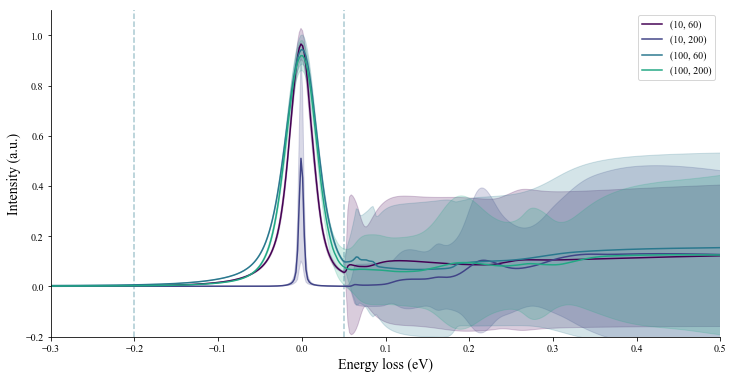
\includegraphics[width=120mm]{plots/extrapolate_energyloss.png}
    \caption{Energy loss extrapolation on vacuum peaks under four different recording settings (exposure time, beam energy). The data within the energy region [-.2, 0.05] eV is known to the network by training. Extrapolation predictions are shown outside this region, marked by the dashed lines.}
    \label{fig:extrapoleloss}
\end{figure}

The goodness of our prediction can be quantified by means of $\chi^2$. So one can separate the parameter space (in Texp and Ebeam for example) into "training" and "prediction" regions, and use one to predict the other. If our error estimate is good, we should find chi2/ndat $\simeq$ 1 also for the predicted datasets


\subsubsection{Beam energy}
\label{sec:ebeam}
The training data contained only two recorded beam energies of 60 and 200 keV. Interpolation and extrapolation predictions have been retrieved on a continuous set of beam energies between 0 and 300 keV. In Fig.~\ref{fig:extrapolbeam} one can observe the mean predicted intensity and mean prediction error, where the average is taken over the energy loss range. The dashed lines indicate the beam energies for which we have data: correspondingly, the errors in these points are small, as the model can make an accurate prediction. The more the beam energy deviates from the known values, the bigger the uncertainties in the predictions become. 

\begin{figure}[H]
    \centering
    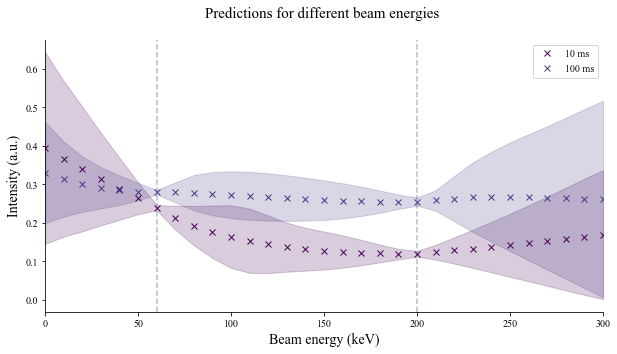
\includegraphics[width=120mm]{plots/Extrapolate_beamenergy.png}
    \caption{Predictions on a continuous set of beam energies, while inputs for energy loss and exposure time are the same as for the training data. The dashed lines indicate the beam energies that are known to the network by training.}
    \label{fig:extrapolbeam}
\end{figure}

\subsubsection{Exposure time}
\label{sec:texp}
The network was trained on data with exposure times of $10$ and $100$ ms, so interpolation and extrapolation is possible. Similar to the predictions for varying beam energy, also for exposure time the uncertainties grow bigger as the value deviates more from the training inputs.

\begin{figure}[H]
    \centering
    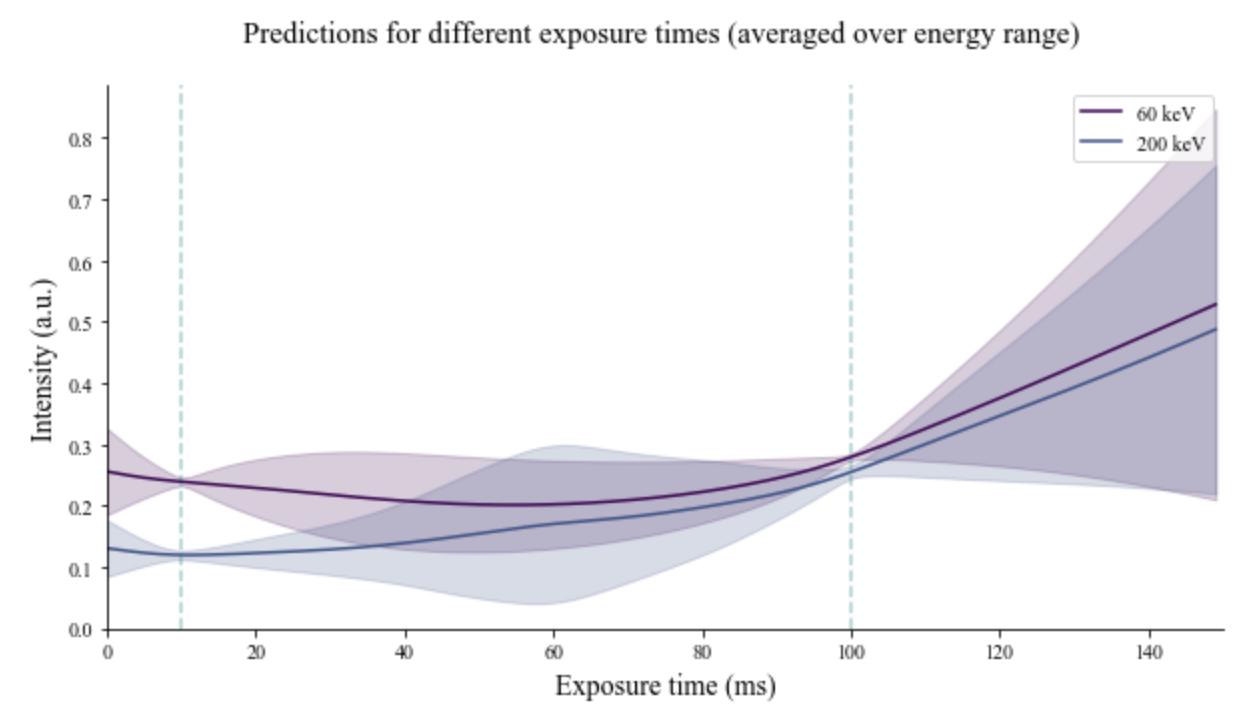
\includegraphics[width=120mm]{plots/Extrapolate_exposuretime.png}
    \caption{Predictions on a continuous set of exposure time, while inputs for energy loss and beam energy are the same as for the training data. The dashed lines indicate the exposure times known to the network by training.}
    \label{fig:extrapolbeam}
\end{figure}


% Discussion of the results in sample
\section{ZLP subtraction and bandgap determination in WS$_2$}
\label{sec:results_sample}

Following the discussion of the vacuum results, we now move
to present the application of our fitting strategy to the parametrisation
of EEL spectra recorded on samples.
%
Specifically, we will analyse EELS measurements taken on the WS$_2$ nanostructures
presented in~\cite{SabryaWS2} and reviewed in Sect.~\ref{sec:tmd}.
%
These nanostructures exhibit a flower-like configuration where different layers
of material combine to form the petals and the stem of the flowers.
%
Their geometrical configuration is such that, depending on the specific region
of the nanostructure that one is imaging, the spectra will be sensitive
to different thicknesses and orientations of the material.

The parametrisation of these in-sample EEL spectra will then be used
to subtract the ZLP contribution and extract the bandgap energy $E_{\rm BG}$ from
the behaviour of $I_{\rm inel}(\Delta E)$ in the onset region.
%
The value of the bandgap  has been estimated in different ways
from subtracted EEL spectra, such as by means of the inflection point of the rising intensity or
a linear fit to the maximum positive slope~\cite{Schamm:2003}.
%
Here we will adopt the approach of~\cite{Rafferty:2000} whereby the behaviour
of $I_{\rm inel}(\Delta E)$ in the onset region is  modeled by
\begin{equation}
  \label{eq:I1}
    I_{\rm inel}(\Delta E) \simeq  A \lp \Delta E-E_{\rm BG} \rp^{b} \, , \quad \Delta E \ge E_{\rm BG} \, ,
\end{equation}
and vanishes for $E < E_{\rm BG}$, where $A$ and $b$ are constants extracted from the fit.
%
The power exponent $b$ is expected to be $b\simeq 1/2$ for a semiconductor material characterised
by a direct bandgap, and $b\simeq 3/2$ for the case instead of an indirect bandgap.

\subsection{Training dataset}
%
Fig.~\ref{fig:ws2positions} displays
low-magnification TEM images of two different regions of
the WS$_2$ nanoflowers, denoted as sample A and sample B in the following.
%
In each image we indicate the specific locations where
EEL spectra have been recorded, including in-vacuum measurements taken
for calibration purposes.
%
In the upper image, the differences in contrast are correlated to the material
thickness, with higher contrast corresponding to thinner regions.
%
Here the ZLP parametrisation strategy will be applied separately
to samples A and B, since in each case the EELS measurements have
been obtained with different electron microscopes and
operation settings, which thus as explained in Sect.~\ref{sec:eels}
must be analysed independently.

%%%%%%%%%%%%%%%%%%%%%%%%%%%%%%%%%%%%%%%%%%%%%%%%%%%%%%%%%%%%%%%%%%%%%%%
\begin{figure}[t]
\begin{centering}
  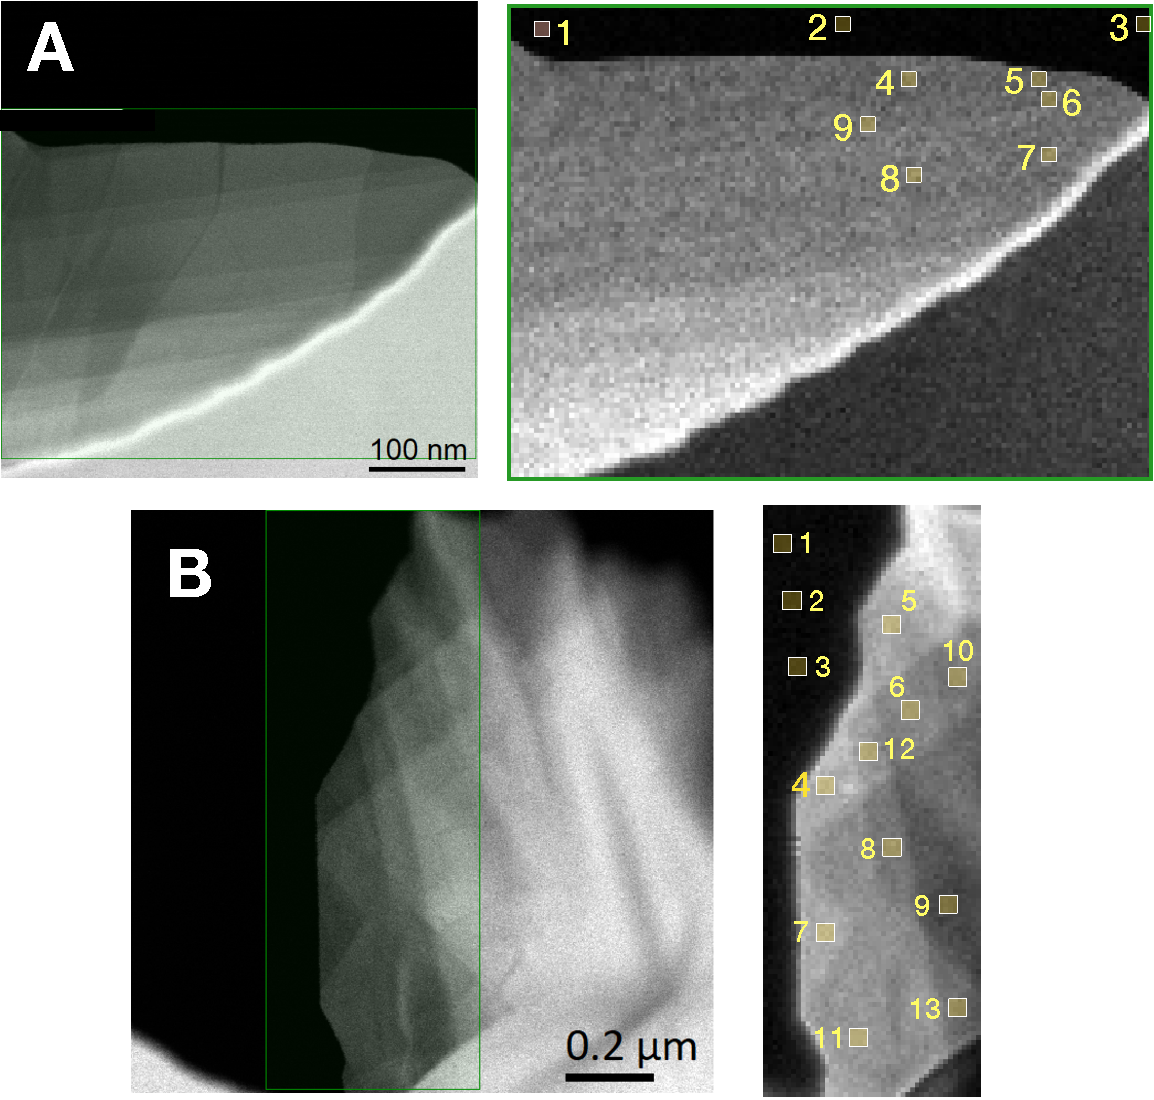
\includegraphics[width=0.87\linewidth]{plots/Spectra_location.pdf}
  \caption{Low-magnification TEM images of two different regions of
    the WS$_2$ nanoflowers, denoted as sample A and sample B respectively.
    %
    In each image we indicate the locations where
    EEL spectra have been recorded, including the in-vacuum measurements taken
    for calibration purposes.
    %
    In sample A the difference in contrast is correlated to the material
    thickness, with higher contrast corresponding to thinner regions of the nanostructure.
  }
\label{fig:ws2positions}
\end{centering}
\end{figure}
%%%%%%%%%%%%%%%%%%%%%%%%%%%%%%%%%%%%%%%%%%%%%%%%%%%%%%%%%%%%%%%%%%%%%%%%%%

In Table~\ref{table:sampledata} we demonstrate the most relevant properties of the spectra collected
in the locations indicated in Fig.~\ref{fig:ws2positions} using the same convention as
in Table~\ref{table:sampledata}.
%
As mentioned, the sets of spectra from samples A and B
have been acquired with different microscopes and are therefore
not directly comparable.
%
The full width at half maximum is averaged over all spectra of a given set,
including those acquired on vacuum.
%
From this table one can observe that the microscope resolution on the measurements of the first set equals 160 meV, 
which is three times higher
than the resolution obtained on the second set. 
%
This difference can be ascribed to the fact that the first set of measurements were obtained with the use of a 
monochromator, whereas the spectra of set B were recorded without a monochromator.
%

%%%%%%%%%%%%%%%%%%%%%%%%%%%%%%%%%%%%%%%%%%%%%%%%%%%%%%%%%%%%%%%%%%%%%%%%%%%%%%%%%%%%%%%%%%%%%
%%%%%%%%%%%%%%%%%%%%%%%%%%%%%%%%%%%%%%%%%%%%%%%%%%%%%%%%%%%%%%%%%%%%%%%%%%%%%%%%%%%%%%%%%%%%%
\begin{table}[t]
  \begin{center}
            \renewcommand{\arraystretch}{1.50}
  \begin{tabular}{@{}ccccccccc}
\br
Set & $t_{\rm exp}$ {(}ms{)} & $E_{\rm b}$ {(}keV{)} & $N_{\rm sp}$ & $N_{\rm dat}$ & $\Delta E_{\rm min}$~(eV)  & $\Delta E_{\rm max}$~(eV)  & FWHM~(eV)  \\ 
\mr
A        &       ?       &    200 keV       &   10     &    2000    &     -0.93        & 9.07   & $ 0.16\pm0.01$ \\
B        &       ?       &        ?         &   6      &    1918    &     -4.054       & 45.471 & $ 0.47\pm0.01$  \\
\br
  \end{tabular}
    \end{center}
  \caption{\small Same as Table~\ref{table:vacuumdata} now for the EEL spectra taken on two sets of WS$_2$ nanostructures. \textbf{ToDo: missing operational values}
  }
   \label{table:sampledata}
\end{table}
%%%%%%%%%%%%%%%%%%%%%%%%%%%%%%%%%%%%%%%%%%%%%%%%%%%%%%%%%%%%%%%%%%%%%%%%%%%%%%%%%%%%%%%%%%%%%%%%%5
%%%%%%%%%%%%%%%%%%%%%%%%%%%%%%%%%%%%%%%%%%%%%%%%%%%%%%%%%%%%%%%%%%%%%%%%%%%%%%%%%%%%%%%%%%%%%

In the following we will focus on representative spectra, specifically spectra \#4 and \#5 in sample
A and spectra \#14 and \#15 in sample B.
%
The full set of original spectra are made available together with the code used to
analyse them as described in this work, whose installation
and usage instructions are summarised in~\ref{sec:installation}.
%
By means of the {\tt Digital Micrograph} EELS software we can determine
the thickness of the material in each of the locations, and use it to
estimate the number of monolayers, taking into account that
one layer (S-W-S) of WS$_2$ has a thickness of around 0.9 nm.
%
For example, the thinner spectrum in sample A is \#5,
with a thickness of 2.1 nm corresponding to around 2 monolayers.

\subsection{ZLP subtraction}

In Table~\ref{table:sampledata_summary} we display
the mean value and uncertainty of the first local minima, $\Delta E|_{\rm min}$,
   averaged over the spectra corresponding to samples A and B from
    Fig.~\ref{fig:ws2positions},
as well as the corresponding values of the hyper-parameters
    $\Delta E_{\rm I}$ and $\Delta E_{\rm II}$ defined in Fig.~\ref{fig:EELS_toy}.
    %
Recall that as explained in Sect.~\ref{sec:methodology} only
the data with $\Delta E \le \Delta E_{\rm I}$ is used for the training
    of the neural network model.
    %
    For $\Delta E \ge \Delta E_{\rm II}$ instead, the training set includes only the pseudo-data
    that implements the $I_{\rm ZLP}(\Delta E)\to 0$ constraint.

%%%%%%%%%%%%%%%%%%%%%%%%%%%%%%%%%%%%%%%%%%%%%%%%%%%%%%%%%%%%%%%%%%%%%%%%%%%%%%%%%%%%%%%%%%%%%
%%%%%%%%%%%%%%%%%%%%%%%%%%%%%%%%%%%%%%%%%%%%%%%%%%%%%%%%%%%%%%%%%%%%%%%%%%%%%%%%%%%%%%%%%%%%%
\begin{table}[t]
  \begin{center}
            \renewcommand{\arraystretch}{1.50}
  \begin{tabular}{@{}ccccccccc}
\br
Set & $\Delta E|_{\rm min}$~(eV)  &  $\Delta E_{\rm I}$~(eV)  &  $\Delta E_{\rm II}$~(eV)   \\
\mr
A        &    $1.80\pm0.04$               &          1.4        &      6        \\
B        &    $2.70\pm0.06$               &          1.8        &      12         \\
\br
  \end{tabular}
    \end{center}
  \caption{\small The mean value and uncertainty of the first local minima, $\Delta E|_{\rm min}$,
    averaged over the spectra corresponding to samples A and B from
    Fig.~\ref{fig:ws2positions}.
    %
    We also indicate
     the corresponding values of the hyper-parameters
     $\Delta E_{\rm I}$ and $\Delta E_{\rm II}$ defined in Fig.~\ref{fig:EELS_toy} used for the training
     of the neural network model.
    %
  }
   \label{table:sampledata_summary}
\end{table}
%%%%%%%%%%%%%%%%%%%%%%%%%%%%%%%%%%%%%%%%%%%%%%%%%%%%%%%%%%%%%%%%%%%%%%%%%%%%%%%%%%%%%%%%%%%%%%%%%5
%%%%%%%%%%%%%%%%%%%%%%%%%%%%%%%%%%%%%%%%%%%%%%%%%%%%%%%%%%%%%%%%%%%%%%%%%%%%%%%%%%%%%%%%%%%%%

 We observe that the location of the first minimum is relatively stable
 among all the spectra belonging to a given set.
 %
 The neural network training is performed for a wide range of $\Delta E_{\rm I}$ values
 subject to the condition that $\Delta E_{\rm I} \le \Delta E_{\rm min}$.
 %
 The optimal values listed  in Table~\ref{table:sampledata_summary} are selected
 by means of comparing the intensity derivatives in the sample with those
 of the vacuum combined with a stability analysis, as we discuss below.
 %
 Upon completion of the neural network training, one ends up
 for each of the independent samples with
 a set $N_{\rm rep}=500$ replicas
 of the zero-loss peak parametrisation, $I_{\rm ZLP}^{({\rm mod})(k)}(\Delta E)$.
 %
 Assuming that we have $N_{\rm sp}$ spectra in each sample, then the zero-loss peak
 subtraction is performed individually
 for each Monte Carlo replica,
 \be
 \label{eq:subtractedModelPrediction}
 I_{\rm inel}^{({\rm mod})(j,k)}(\Delta E) \equiv I_{\rm EELS}^{(j)}(\Delta E) - I_{\rm ZLP}^{({\rm mod})(k)}(\Delta E)\, ,
 \quad \forall~N_{\rm rep} \, ,\quad j=1,\ldots,N_{\rm sp} \, ,
 \ee
 from which statistical estimators can be evaluated as usual.
 %
 For instance, the mean value for our model prediction for the $j$-th spectrum
 can be evaluated by averaging over the set of replicas,
 \be
 \la  I_{\rm inel}^{({\rm mod})(j)}\ra (\Delta E)
 = \frac{1}{N_{\rm rep}} \sum_{k=1}^{N_{\rm rep}}  I_{\rm inel}^{({\rm mod})(j,k)}(\Delta E) \, ,
 \quad j=1,\ldots,N_{\rm sp} \, ,
 \ee
 and likewise for the corresponding uncertainties.
%
 We note that for large values of $\Delta E$
 the model prediction reduces to the original spectra, since in that region
 the ZLP contribution vanishes by construction,
 \be
 I_{\rm inel}^{({\rm mod})(j,k)}(\Delta E \gg \Delta E_{\rm II}) \to  I_{\rm EELS}^{(j)}(\Delta E) \, ,\quad
 \forall~j,k \, .
 \ee
 
 For very small values of the energy loss $\Delta E$, the contribution to the total
 spectra from inelastic scatterings is negligible
 and thus the subtracted model prediction Eq.~(\ref{eq:subtractedModelPrediction}) should
 vanish.
 %
 However, this will not be the case in practice since the neural-net model is trained on
 the $N_{\rm sp}$ ensemble of spectra, rather that just on individual ones, and thus the expected
 $\Delta E \to 0$ behaviour will only be achieved within uncertainties rather than at the level of
 central values.
 %
 To achieve the desired $\Delta E \to 0$ limit, we apply a matching procedure
 as follows.
 %
 We introduce another hyper-parameter, $\Delta E_0 < \Delta E_1$, such that
 one has for the $k$-th ZLP replica associated to the $j$-th spectrum the following
 behaviour:
 \bea
 \nonumber
 I_{\rm ZLP}^{({\rm mod})(j,k)}(\Delta E) &=& I_{\rm EELS}^{(j)}(\Delta E) \, ,\quad \Delta E < \Delta E_0  \, ,\\
 I_{\rm ZLP}^{({\rm mod})(j,k)}(\Delta E) &=& I_{\rm EELS}^{(j)} + \lp \xi_1^{(n_l)(k)}(\Delta E) - I_{\rm EELS}^{(j)}(\Delta E)\rp  \times \mathcal{F} \, , \nonumber \quad 
 \Delta E_0 < \Delta E \le \Delta E_1 \, ,\\
 &&\mathcal{F} = \exp\lp -\frac{\lp \Delta E - \Delta E_1 \rp^2 }{\lp \Delta E_0 - \Delta E_1 \rp^2 \delta^2} \rp  \, , \label{eq:matching} \\
 I_{\rm ZLP}^{({\rm mod})(j,k)}(\Delta E) &=& \xi_1^{(n_l)(k)}(\Delta E) \, , \quad \Delta E > \Delta E_1 \nonumber \, ,
 \eea
 where $\xi_1^{(n_l)(k)}$ indicates the output of the $k$-th neural network that parametrises
 the ZLP and $\delta$ is a dimensionless tunable parameter.
 %
 In Eq.~(\ref{eq:matching}), $\mathcal{F}(\Delta E)$ represents a matching factor
 that ensures that the model prediction of the zero loss peak smoothly interpolates
 between $\Delta E=\Delta E_0$ (where $\mathcal{F}\ll 1$ and the original spectrum should
 be reproduced) and $\Delta E=\Delta E_1$
 (where $\mathcal{F}=1$ leaving the neural net output unmodified).
 %
 In  this work we choose $\Delta E_0 = \Delta E_1 -0.5\,{\rm eV}$, though we have verified
 that results are fairly independent of this choice.

 Taking into account the matching procedure, we can slightly modify Eq.~(\ref{eq:subtractedModelPrediction})
 to read
 \be
 \label{eq:subtractedModelPrediction2}
 I_{\rm inel}^{({\rm mod})(j,k)}(\Delta E) \equiv I_{\rm EELS}^{(j)}(\Delta E) - I_{\rm ZLP}^{({\rm mod})(j,k)}(\Delta E)\, ,
 \quad \forall~N_{\rm rep} \, ,\quad j=1,\ldots,N_{\rm sp} \, .
 \ee
 For each of the $N_{\rm sp}$ collected spectra and each of the $N_{\rm rep}$ replicas,
 we fit to Eq.~(\ref{eq:subtractedModelPrediction2}) the functional form Eq.~(\ref{eq:I1}).
 %
 The range in $\Delta E$ for these fits to the subtracted spectra is taken to be
 $\lc \Delta E_{\rm I} - 0.5~{\rm eV}, \Delta E_{\rm I} + 1.2~{\rm eV}\rc$.
 %
 This range has been chosen to maximise the amount of information in the onset region.
 %
 For each of the $N_{\rm sp}$ spectra, we end up with $N_{\rm rep}$ values for
 the bandgap energy and fit exponent,
 \be
 \Big \{ E_{\rm BG}^{(j,k)}, b^{(j,k)} \Big\} \, , \quad k=1,\ldots,N_{\rm rep} \, ,
 \ee
 from which again one can evaluate statistical estimators such as medians, 68\% CL ranges
 and correlations.

The left panel of Fig.~\ref{fig:sp4_subtracted_spectrum} displays
the original
and subtracted EEL spectrum corresponding to location \#4 in Fig.~\ref{fig:ws2positions},
together with the predictions of the ZLP model evaluated using
Eq.~(\ref{eq:mathcing}).
  %
Both for the ZLP model and for the subtracted spectrum we show both the central value
and the standard deviation of the predictions.
%
One can observe how uncertainties are negligible at low $\Delta E$
(due to the matching condition) and large $\Delta E$ (where the ZLP vanishes).
%
It is also possible to verify {\it a posteriori} that the choice of $\Delta E_I$
is sensible, by evaluating the following ratio
\be
\mathcal{R}_{\rm abs}\lp \Delta E_1\rp \equiv 
\la I_{\rm ZLP}^{({\rm mod})(j)}\ra /I_{\rm EELS}^{(j)} \Big|_{\Delta E = \Delta E1} \, .
\ee
One should verify that $\mathcal{R}_{\rm abs}\lp \Delta E_1\rp$ is not too far from unity,
indicating that the training dataset has not been contaminated by the inelastic contributions.
     

%%%%%%%%%%%%%%%%%%%%%%%%%%%%%%%%%%%%%%%%%%%%%%%%%%%%%%%%%%%%%%%%%%%%%%%
\begin{figure}[t]
\begin{centering}
  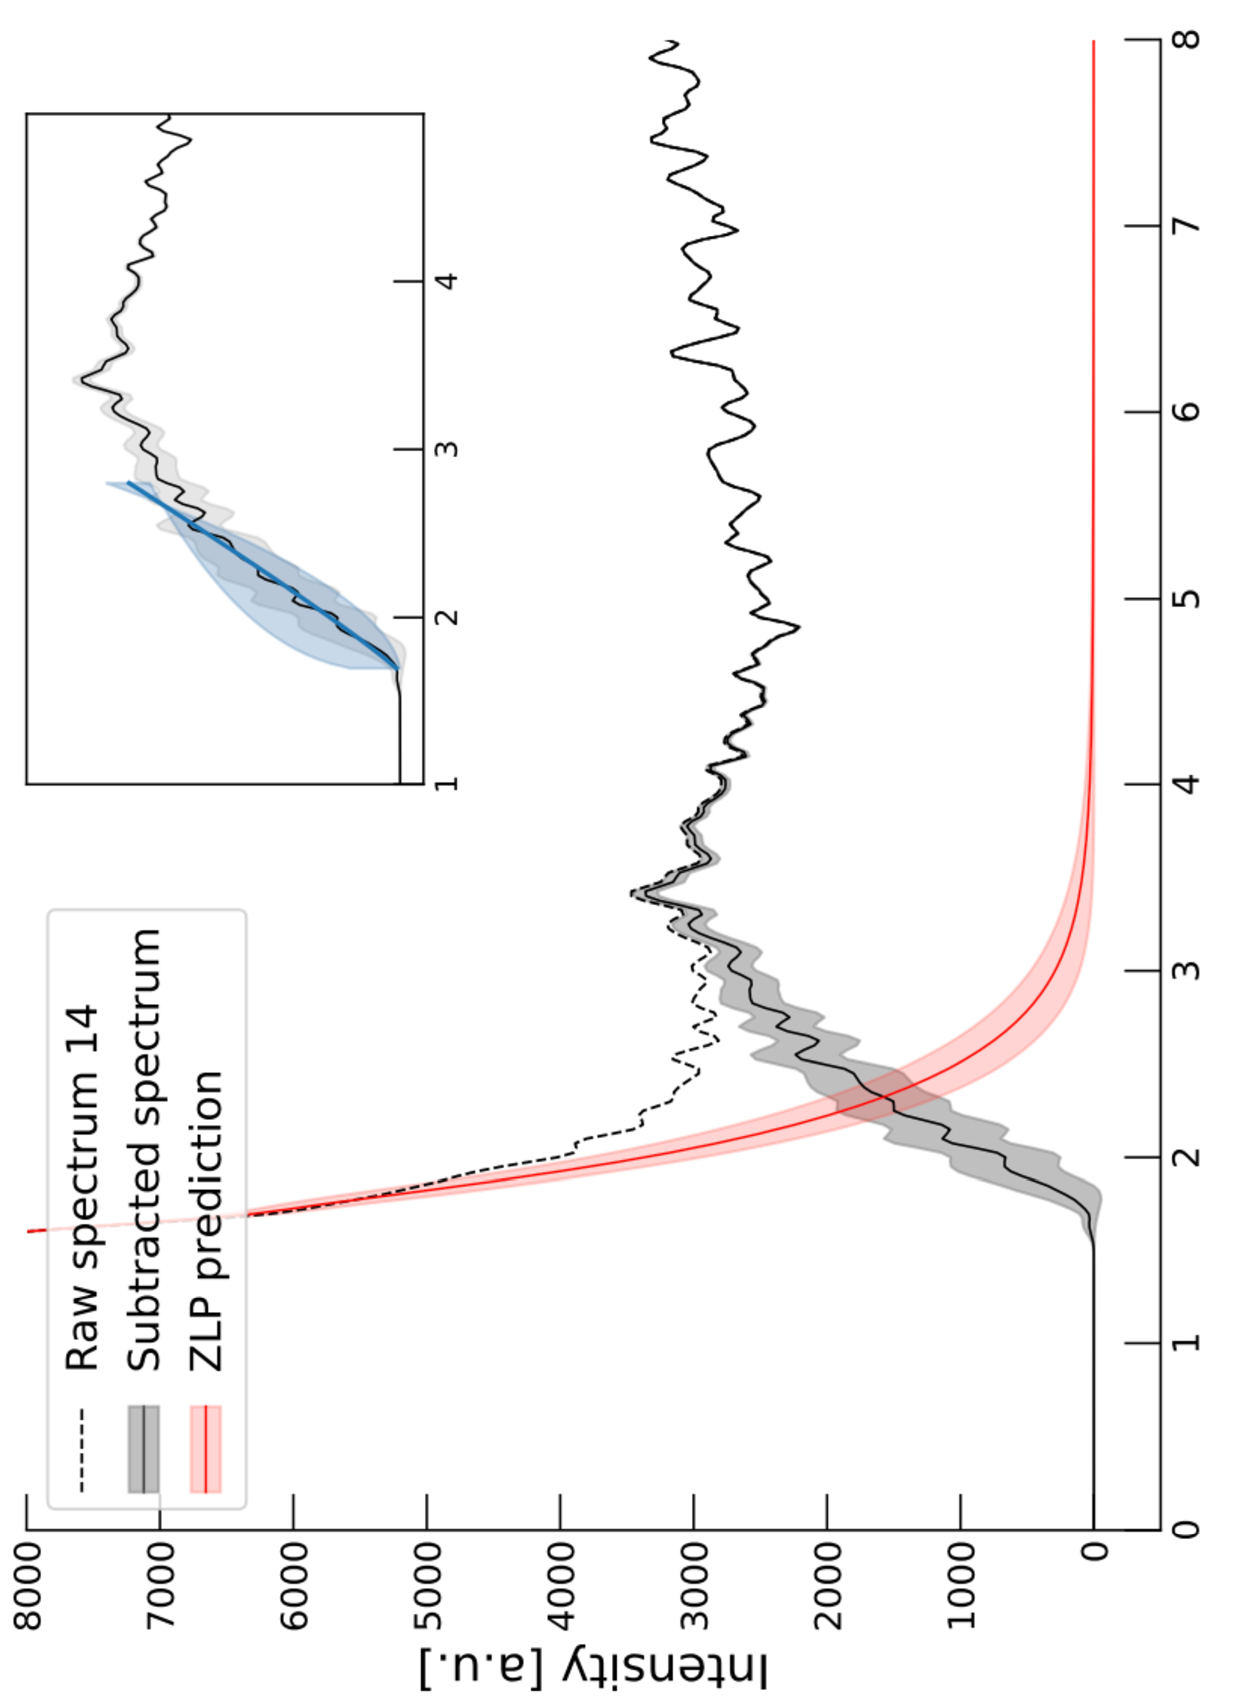
\includegraphics[width=0.36\linewidth,angle=-90]{plots/sp4_subtracted_spectrum.pdf}
   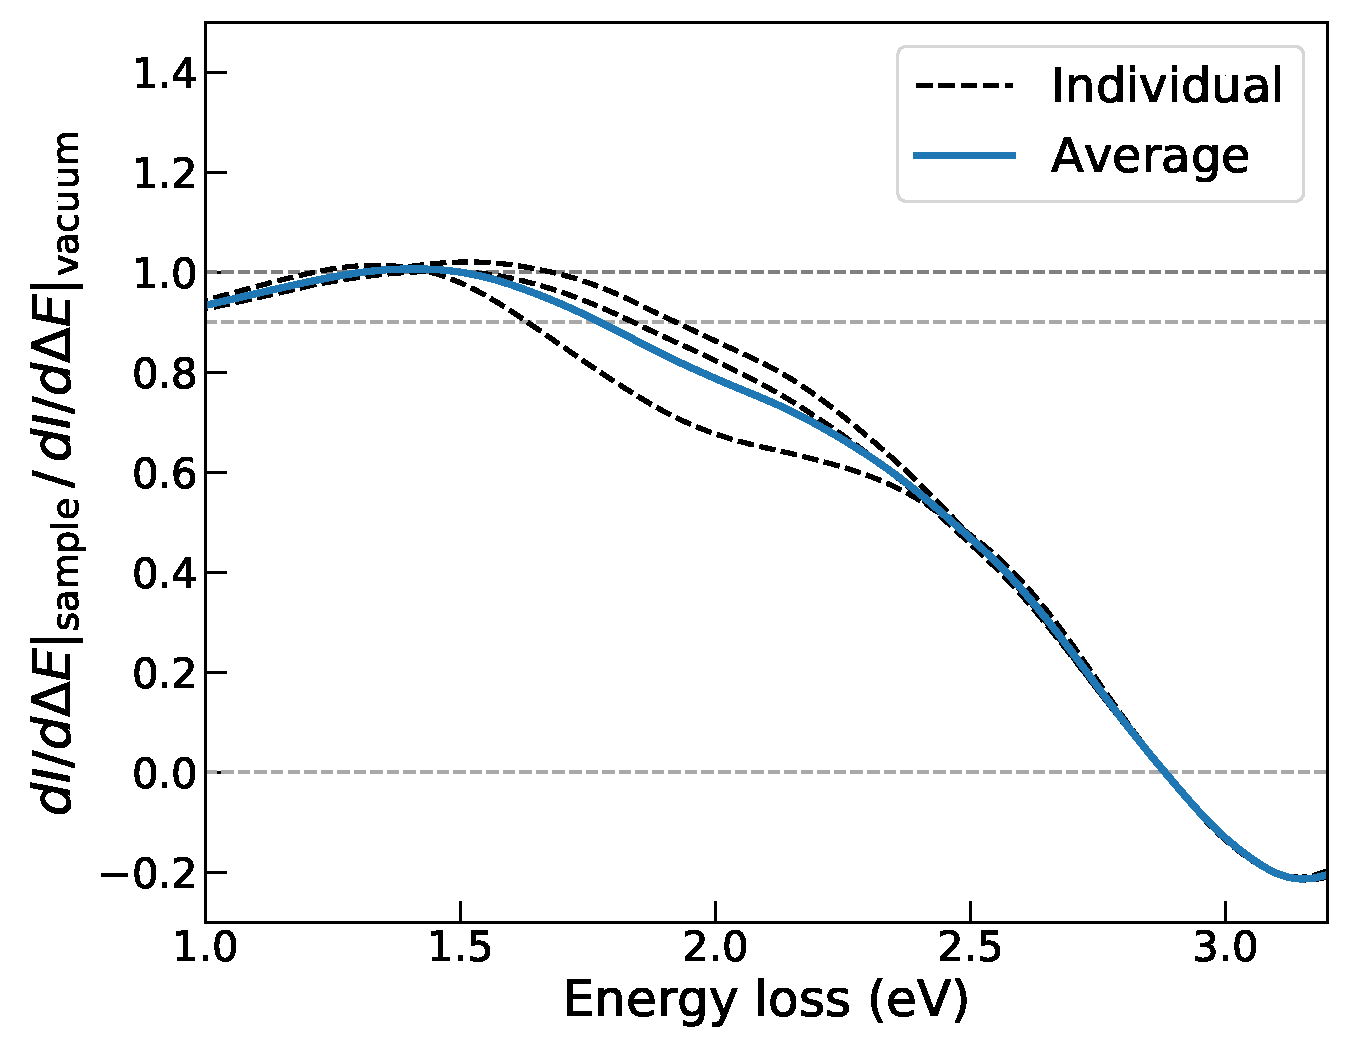
\includegraphics[width=0.36\linewidth,angle=-90]{plots/Derivatives_sp4.pdf}
   \caption{Left: the original
     and subtracted EEL spectrum corresponding to location \#4 in Fig.~\ref{fig:ws2positions},
     together with the predictions of the ZLP models.
     %
     The inset displays the result of the fit using Eq.~(\ref{eq:I1}) to the onset
     region of the subtracted spectrum.
     %
     Right: The ratio of the derivative intensity of the original spectrum, $dI_{\rm EEL}/d\Delta E$,
     over that of the ZLP measurements taken on the vacuum $d I_{\rm ZLP}/d\Delta E$.
  }
\label{fig:sp4_subtracted_spectrum}
\end{centering}
\end{figure}
%%%%%%%%%%%%%%%%%%%%%%%%%%%%%%%%%%%%%%%%%%%%%%%%%%%%%%%%%%%%%%%%%%%%%%%%%%

The inset in the left panel of Fig.~\ref{fig:sp4_subtracted_spectrum}
shows the result of the  fits using Eq.~\ref{eq:I1} to the subtracted spectrum,
with the band indicating the 68\% CL uncertainties.
%
We discuss below the implication of this fit for the bandgap determination
in the WS$_2$ nanostructures.

In the right panel of  Fig.~\ref{fig:sp4_subtracted_spectrum} we display the ratio
between the derivative of the intensity profiles corresponding to the sample locations
with respect to a reference measurement taken on vacuum,
\be
\mathcal{R}_{\rm der}(\Delta E) \equiv 
\frac{
  dI_{\rm EELS}^{(j)}/ d\Delta E
}{
  dI_{\rm EELS}^{(j')} /d\Delta E
}\lp \Delta E\rp \, ,
\ee
where $j'$ labels one of the vacuum spectra.
%
This ratio allows to identify a suitable value of $\Delta E_{I}$ by determining
for which energy losses the derivatives of the sample spectra deviate significantly
from the vacuum ones.
%
Note that $\mathcal{R}_{\rm der}(\Delta E)=0$ indicates the position of the first
local minimum of the spectra.
%
From this comparison we can see that Fig.~\ref{fig:sp4_subtracted_spectrum} validates our choice of
$\Delta E_{\rm I}$.

\subsection{Bandgap determination}

We now move to discuss the results on the bandgap determination obtained
by fitting the functional form Eq.~(\ref{eq:I1}) to each of the subtracted
spectra defined by Eq.~(\ref{eq:subtractedModelPrediction2}).
%
Results will be presented as a function of the hyper-parameter $\Delta E_{\rm I}$
in order to gauge the stability of the results.
%
To begin with, in Fig.~\ref{fig:bvalues}
we display the values of the bandgap energy $E_{\rm BG}$ (top panels)
and of the exponent $b$ (bottom panels) as a function of $\Delta E_I$
for locations \#4 (left)
and \#5 (right panels) from Sample A indicated in Fig.~\ref{fig:ws2positions}.
%
The central value and the error band for each value of $\Delta E_I$ is evaluated
as the median and the 68\% CL interval over the $N_{\rm rep}=500$ Monte Carlo replicas.
%
The red marker indicates the position of the optimal value of
$\Delta E_{\rm I}$ determined as specified above.

%%%%%%%%%%%%%%%%%%%%%%%%%%%%%%%%%%%%%%%%%%%%%%%%%%%%%%%%%%

\begin{figure}[t]
\begin{centering}
  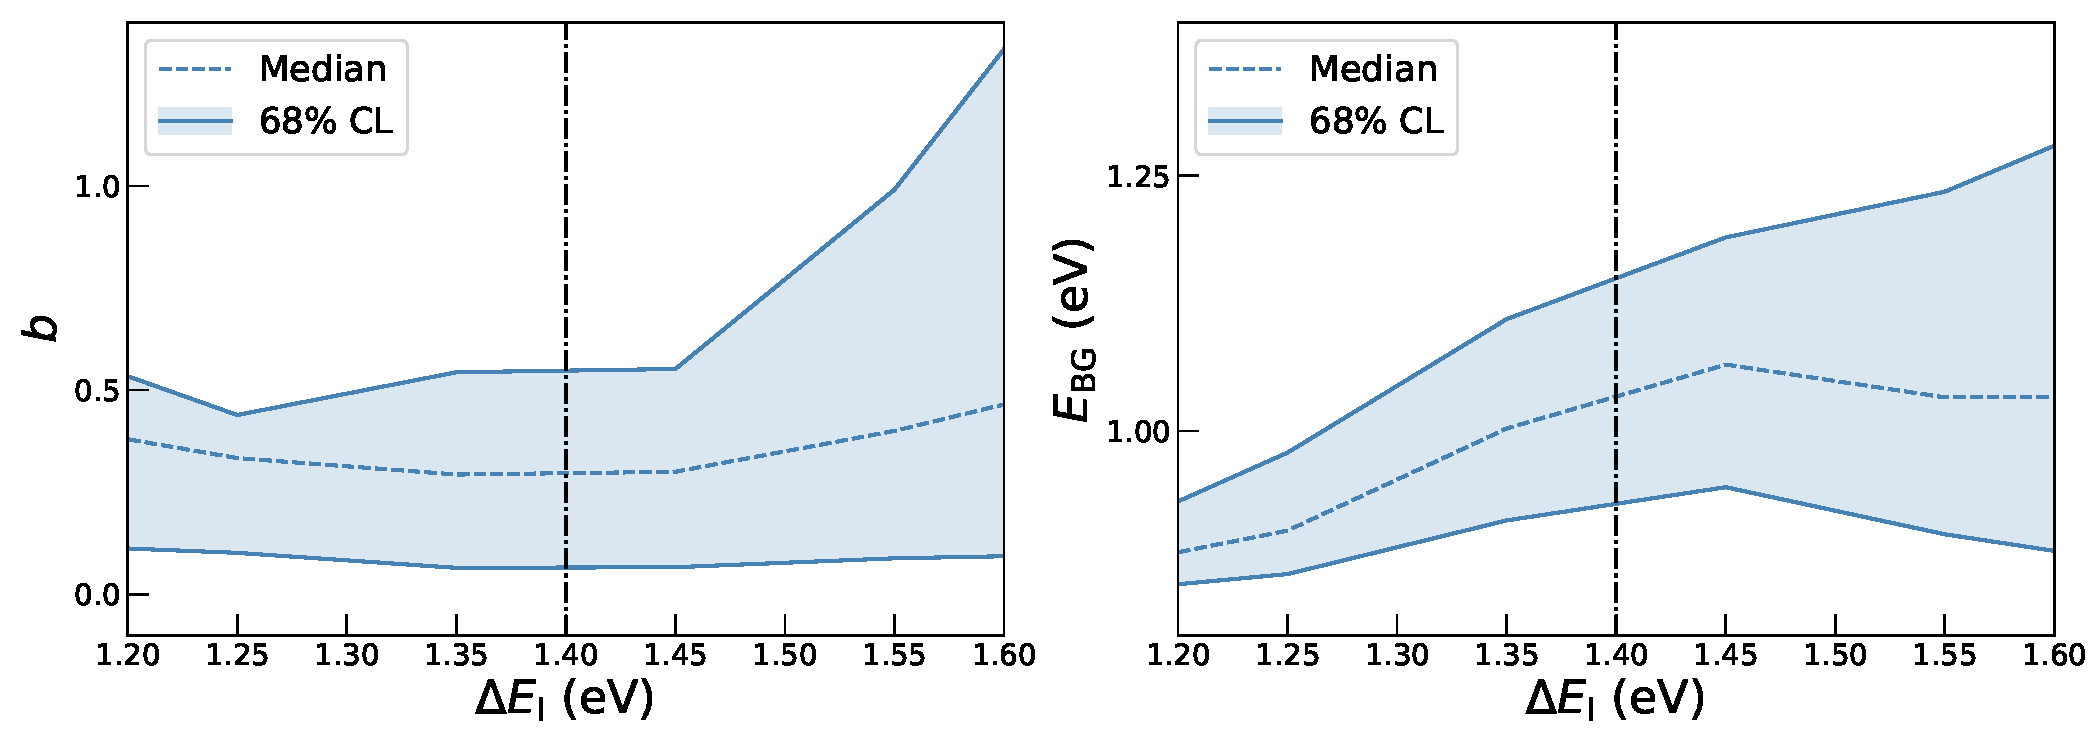
\includegraphics[width=0.6\linewidth]{plots/Stabilityplots_sp4.pdf}
  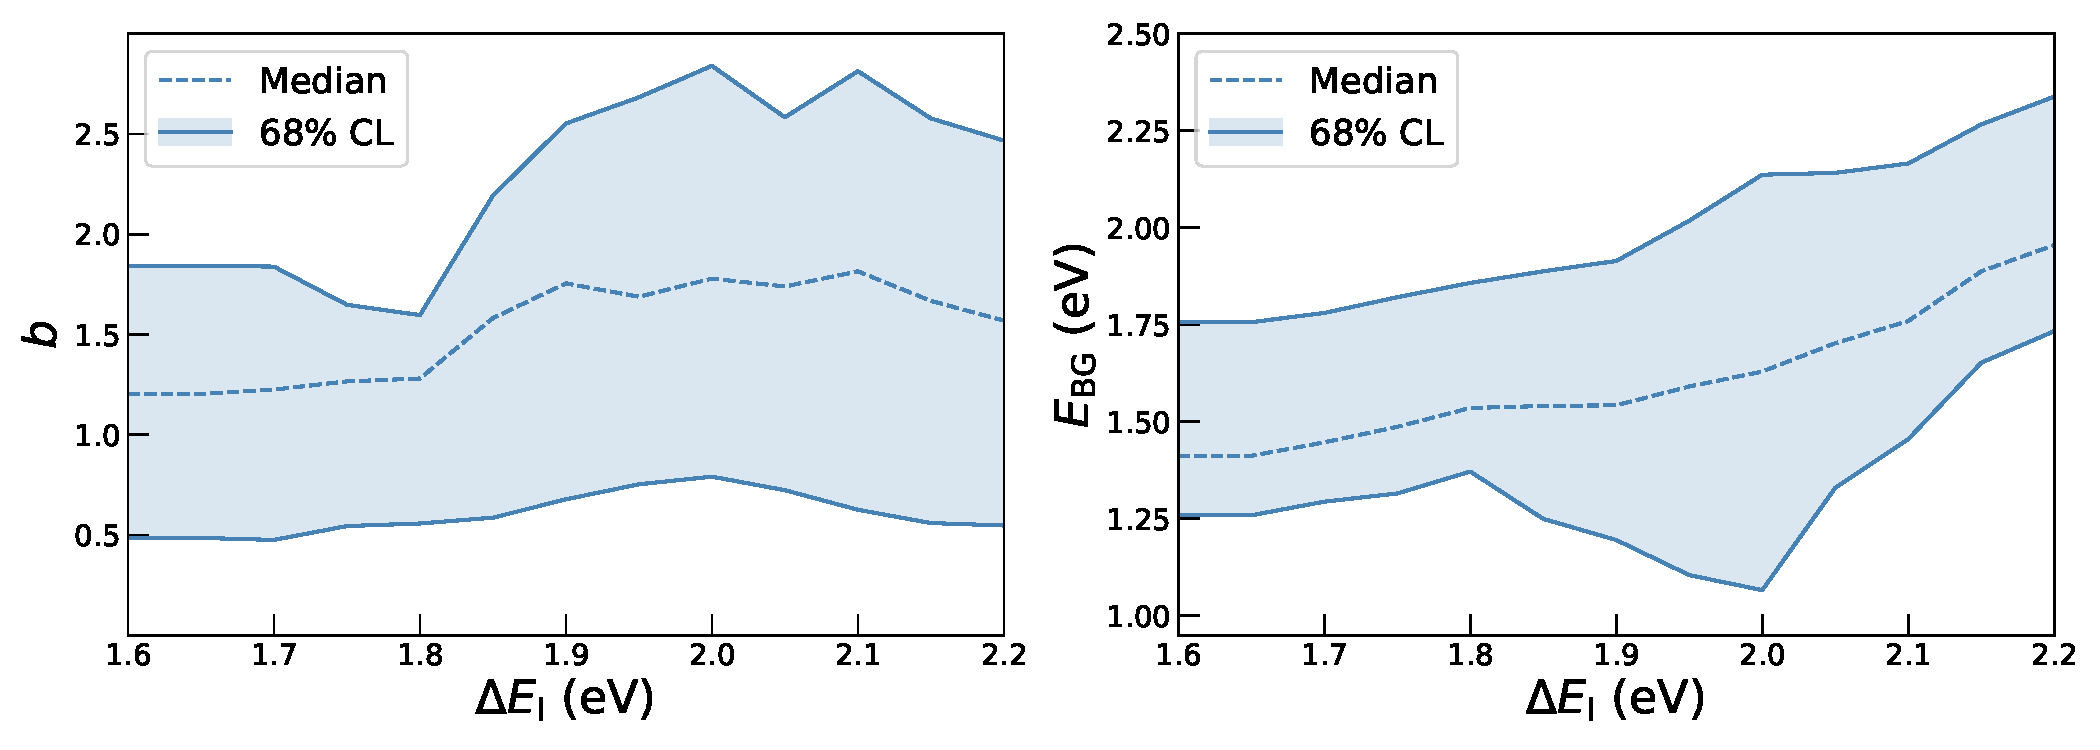
\includegraphics[width=0.6\linewidth]{plots/Stability_plots_sp14.pdf} 
  \caption{Top: the values of the bandgap energy $E_{\rm BG}$ and of the exponent $b$
  obtained from fits to the onset
  region of subtracted spectra using Eq.~(\ref{eq:I1}) as a function
  of the hyper-parameter $\Delta E_{\rm I}$.
  %
  We show results for locations \#4 from set A (top)
  and \#14 of set B (bottom) indicated in Fig.~\ref{fig:ws2positions}.
  %
  The central value and the error band for each value of $\Delta E_I$ is evaluated
  as the median and the 68\% CL interval over the $N_{\rm rep}=500$ Monte Carlo replicas.
  }
\label{fig:bvalues}
\end{centering}
\end{figure}
%%%%%%%%%%%%%%%%%%%%%%%%%%%%%%%%%%%%%%%%%%%%%%%%%%%%%%%%%%%%%

In Table~\ref{table:bandgap_fitting} we collect
 the median values and 68\% CL ranges for the bandgap energy $E_{\rm BG}$
 and the bandgap exponent $b$ determined from fitting Eq.~(\ref{eq:I1}) to each of the subtracted
 spectra defined by Eq.~(\ref{eq:subtractedModelPrediction2}).
 %
 We consider two representative spectra from sample A and two
 from sample B. 
 %
 The error is divided into the statistical and the systematic component, which are
 then added in quadrature to evaluate the total uncertainty in the fit results. 
 %
 From these results we see that the spectra in sample A are consistent with a direct bandgap,
 while those of sample B with an indirect bandgap.

%%%%%%%%%%%%%%%%%%%%%%%%%%%%%%%%%%%%%%%%%%%%%%%%%%%%%%%%%%%%%%%%%%%%%%%%%%%%%%%%%%%%%%%%%%%%%
%%%%%%%%%%%%%%%%%%%%%%%%%%%%%%%%%%%%%%%%%%%%%%%%%%%%%%%%%%%%%%%%%%%%%%%%%%%%%%%%%%%%%%%%%%%%%
\begin{table}[t]
  \begin{center}
    \footnotesize
            \renewcommand{\arraystretch}{1.50}
  \begin{tabular}{@{}c|c|c|c}
\br
Set & Spectrum   &$E_{\rm BG}$~(eV)  &  $b$  \\
\mr
\mr
A        &   sp\#4   &     $ 2.0 \pm 0.3^{\rm (stat)} \pm  0.2^{\rm (sys)}=  2.0 \pm 0.3^{\rm (tot)}   $                &       $ 0.5 \pm 0.3^{\rm (stat)} \pm  0.2^{\rm (sys)}=  0.5 \pm 0.3^{\rm (tot)}   $                       \\
\mr
A        &   sp\#5   &     $ 2.0 \pm 0.3^{\rm (stat)} \pm  0.2^{\rm (sys)}=  2.0 \pm 0.3^{\rm (tot)}   $                &       $ 0.5 \pm 0.3^{\rm (stat)} \pm  0.2^{\rm (sys)}=  0.5 \pm 0.3^{\rm (tot)}   $                       \\
\mr
\mr
B        &   sp\#14   &     $ 2.0 \pm 0.3^{\rm (stat)} \pm  0.2^{\rm (sys)}=  2.0 \pm 0.3^{\rm (tot)}   $                &       $ 0.5 \pm 0.3^{\rm (stat)} \pm  0.2^{\rm (sys)}=  0.5 \pm 0.3^{\rm (tot)}   $                       \\
\mr
B        &   sp\#15   &     $ 2.0 \pm 0.3^{\rm (stat)} \pm  0.2^{\rm (sys)}=  2.0 \pm 0.3^{\rm (tot)}   $                &       $ 0.5 \pm 0.3^{\rm (stat)} \pm  0.2^{\rm (sys)}=  0.5 \pm 0.3^{\rm (tot)}   $                       \\
\br
  \end{tabular}
    \end{center}
  \caption{\small The median values and 68\% CL ranges for the bandgap energy $E_{\rm BG}$
    and the bandgap exponent $b$ determined from fitting Eq.~(\ref{eq:I1}) to each of the subtracted
    spectra defined by Eq.~(\ref{eq:subtractedModelPrediction2}).
    %
    As justified in the text, we consider two representative spectra from sample A and two
    from sample B. 
    %
    The error is divided into the statistical and the systematic component, which are
    then added in quadrature to evaluate the total uncertainty in the fit results. {\rm ToDo}.
  }
   \label{table:bandgap_fitting}
\end{table}
%%%%%%%%%%%%%%%%%%%%%%%%%%%%%%%%%%%%%%%%%%%%%%%%%%%%%%%%%%%%%%%%%%%%%%%%%%%%%%%%%%%%%%%%%%%%%%%%%5
%%%%%%%%%%%%%%%%%%%%%%%%%%%%%%%%%%%%%%%%%%%%%%%%%%%%%%%%%%%%%%%%%%%%%%%%%%%%%%%%%%%%%%%%%%%%%


% Summary and outlook
%%%%%%%%%%%%%%%%%%%%%%%%%%%%%%%%%%%%%%%%%
\section{Summary and outlook}
%%%%%%%%%%%%%%%%%%%%%%%%%%%%%%%%%%%%%%%%%
\label{sec:summary}

In this work we have presented a novel, model-independent strategy to parametrise and subtract
the ubiquitous zero-loss peak that dominates  the low-loss region
of EEL spectra.


Say somethihg about the connection of our approach with
indirect Dark Matter searches and how we can efficiently
test new materials that can eventually be used
as dark matter detectors.

\subsection*{Acknowledgments}

We are grateful to Emanuele R. Nocera and Jacob J. Ethier for
assistance in installing {\tt EELSfitter} in the Nikhef computing cluster.


\subsection*{Funding}

S.~E.~v.~H. and S.~C.-B. acknowledge financial support
from the ERC through the Starting Grant ``TESLA”'', grant agreement
no. 805021.
%
L.~M. acknowledges support from the
Netherlands Organizational for Scientific Research (NWO)
through the Nanofront program.
%
The work of J.~R. has been partially supported by NWO.

\subsection*{Declaration of competing interest}

The authors declare that they have no known competing financial interests or personal relationships that could have appeared to influence the work reported in this paper.

\subsection*{Methods}

{\justify
The EEL spectra used for the training of the vacuum ZLP model presented in Sect.~\ref{sec:results_vacuum} were collected in a ARM200F Mono-JEOL microscope equipped with a GIF continuum spectrometer and operated at 60 kV and 200 kV. For these measurements, a slit in the monochromator of 2.8 $\mu$m was used.
%
The TEM and EELS measurements acquired in Specimen A for the results presented in
Sect.~\ref{sec:results_sample} were recorded in a JEOL 2100F microscope with a cold field-emission
gun equipped with aberration corrector operated at 60 kV. A Gatan GIF Quantum was used for
the EELS analyses. The convergence and collection semi-angles were 30.0 mrad and 66.7 mrad respectively.
%
The TEM and EELS measurements acquired for Specimen B in Sect.~\ref{sec:results_sample}
were recorded using a JEM ARM200F monochromated microscope operated at 60 kV and equipped with
a GIF quantum ERS. The convergence and collection semi-angles were 24.6 mrad and 58.4 mrad respectively
in this case, and the aperture of the spectrometer was set to 5 mm.}


\bibliography{EELS_ML}
\end{document}





\end{document}
